\documentclass[bibliography=totoc,12pt,a4paper]{scrartcl}
\usepackage{amsmath, amssymb, amsthm}
\usepackage{enumerate}% schicke Nummerierung
\usepackage{graphicx}
\usepackage[english, ngerman]{babel}
\usepackage[T1]{fontenc}
\usepackage{lmodern}
\usepackage{datetime}
\usepackage[utf8]{inputenc}
\usepackage{bigdelim}
\usepackage{multirow}
\usepackage{dsfont}
\usepackage[colorlinks=true,linkcolor=black, citecolor=black]{hyperref}
\usepackage{cite}
\usepackage[nottoc]{tocbibind}
\usepackage{empheq}
\usepackage{fancyhdr}
\usepackage{geometry}
\usepackage{lipsum}
\usepackage{tikz,pgfplots}
\usepackage{nicefrac}
\usepackage{graphicx}
\usepackage{subcaption}
\usetikzlibrary{shapes.misc}
\usetikzlibrary{matrix}
\geometry{a4paper,left=40mm,right=30mm, top=5cm, bottom=5cm} 

\def\@biblabel#1{\textcolor{red}{[#1]}}

\newtheoremstyle{linebreak}   % name
{3pt}                         % Space above
{3pt}                         % Space below
{}                            % Body font
{}                            % Indent amount 1
{\bfseries}                   % Theorem head font
{\newline}                    % Punctuation after theorem head
{.5em}                        % Space after theorem head 2
{}                            % Theorem head spec (can be left empty, meaning ‘normal’)
%\theoremstyle{linebreak}
\newtheoremstyle{exampstyle}
  {\topsep} % Space above
  {\topsep} % Space below
  {} % Body font
  {} % Indent amount
  {\bfseries} % Theorem head font
  {.} % Punctuation after theorem head
  {.5em} % Space after theorem head
  {} % Theorem head spec (can be left empty, meaning `normal')
\theoremstyle{exampstyle}
\newtheorem{defi}{Definition}%[chapter]
\newtheorem{satz}[defi]{Satz}
\newtheorem{theorem}[defi]{Theorem}
\newtheorem{propo}[defi]{Proposition}
\newtheorem{lemma}[defi]{Lemma}
\newtheorem{cor}[defi]{Korollar}
\newtheorem{bem}[defi]{Bemerkung}
\newtheorem{bsp}[defi]{Beispiel}
\newtheorem{folg}[defi]{Folgerung}
%bemerkungen oder Fließtext???
\numberwithin{equation}{section} 
 \newcommand{\newln}{\\&\quad\quad{}}
 \setlength\parindent{0pt}

\renewenvironment{abstract}
 {\small
  \begin{center}
  \bfseries \abstractname\vspace{-.5em}\vspace{0pt}
  \end{center}
  \list{}{%
    \setlength{\leftmargin}{10mm}% <---------- CHANGE HERE
    \setlength{\rightmargin}{\leftmargin}%
  }%
  \item\relax}
 {\endlist}


\usepackage{listings}
\usepackage{color}
 
\definecolor{codegreen}{rgb}{0,0.6,0}
\definecolor{codegray}{rgb}{0.5,0.5,0.5}
\definecolor{codepurple}{rgb}{0.58,0,0.82}
\definecolor{backcolour}{rgb}{0.95,0.95,0.92}
 
\lstdefinestyle{mystyle}{
    backgroundcolor=\color{backcolour},   
    commentstyle=\color{codegreen},
    keywordstyle=\color{magenta},
    numberstyle=\tiny\color{codegray},
    stringstyle=\color{codepurple},
    basicstyle=\footnotesize,
    breakatwhitespace=false,         
    breaklines=true,                 
    captionpos=b,                    
    keepspaces=true,                 
    numbers=left,                    
    numbersep=5pt,                  
    showspaces=false,                
    showstringspaces=false,
    showtabs=false,                  
    tabsize=2
}
 
\lstset{style=mystyle}

\begin{document}

\title{Quasi-Newton Methoden in der Formoptimierung}

\author{Daniel Luft}

  \pagestyle{empty}

  % Titelblatt der Arbeit
  \begin{titlepage}

%    \includegraphics[scale=0.45]{kit-logo.jpg}
    \vspace*{2cm} 

 \begin{center} \large 
    
    %Titel des Seminars
    \vspace*{2cm}

    {\huge Quasi-Newton Methoden in der Formoptimierung}
    \vspace*{2.5cm}
	
  \end{center}
  
	Masterarbeit
	\newline

	zur Erlangung des akademischen Grades eines \newline
	Master of Science
	\newline
	
	eingereicht am Fachbereich IV \newline
	der Universität Trier	
	\newline
	
	von	
	\newline
	
    Daniel Luft
    \newline
    
	Erstgutachter:  Prof. Dr. Volker Schulz \newline
	Zweitgutachter: Dr. Kathrin Welker 
	\newline
	
	Trier, den \today.

	
	
	\hspace{10cm}\vspace{-2cm}
\includegraphics[scale=0.4]{Logo-Uni-Trier.jpg}

\end{titlepage}
\newpage

\vspace{10cm}
Universität Trier - Gebäude E \newline
Fachbereich IV - Mathematik

Universitätsring 19 \newline
D-54296 Trier

\newpage




\section*{Danksagung}

Ich möchte mich an dieser Stelle bei all denen bedanken, die mir während der Erstellung dieser Masterarbeit zur Seite standen. 
\newline

Bei Prof. Dr. Volker Schulz möchte ich mich für die unterhaltsamen und aufschlussreichen Gespräche bedanken. 
\newline 

Meiner Familie und Freunden, vorallem meinen Eltern und Aibi, möchte ich danken, mir bei allen Dingen, ob gut und schlecht, beizuwohnen. 

\newpage

  % Inhaltsverzeichnis
  \tableofcontents

\newpage

  % Ab sofort Seitenzahlen in der Kopfzeile anzeigen
  \pagestyle{headings}
  
\selectlanguage{ngerman}
\begin{abstract}
Die Formoptimierung ist ein für die moderne Industrie immer wichtiger werdendes Teilgebiet der Mathematik. Durch Fortschreiten der technischen Realisierbarkeit und den immer mächtiger werdenden Rechenarchitekturen sind Simulationen, Lösung und Umsetzung von Modellbasierten Ansätzen möglich, die vor einigen Dekaden undenkbar schienen. So wird die Formoptimierung heutzutage beispielsweise zur Optimierung von Bauteilen hinsichtlich ihrer Aerodynamik in \cite{abstract1}, bei Problemen der Magnetostatik in \cite{abstract2}, oder dem Design von Turbinen bei \cite{abstract4}. Aber auch bei weniger bekannten Problemstellungen, etwa dem optimalen Design von Hafenanlagen, wie bei \cite{abstract3}, wo die Form unter anderem bezüglich Kostenintensität, aber auch der auftretenden signifikanten Wellenhöhe, optimiert wird. Ziel dieser Arbeit ist es, das Broyden-Fletcher-Goldstein-Shanno-Verfahren (BFGS-Verfahren), als Beispiel eines Quasi-Newton-Verfahrens, im Kontext der Formoptimierung in einem Programm, welches künftig weiter verwendet werden kann, aufzusetzen und zu analysieren. Hierfür werden wir in 
Kapitel \ref{Chapter_grundlagenpde} und \ref{Chapter_formopt} die für uns relevanten theoretischen Bausteine aus der Theorie der Differentialgleichungen und der Formoptimierung legen. In Kapitel \ref{Chap_3} bauen wir auf das vorangegangene auf, und führen in die moderne Betrachtung der Formoptimierung auf Basis von Formräumen ein. Wir zeigen, wie man Metriken auf diesem Raum definiert, und so zugehörige Gradienten erzeugen kann. Anschließend geben wir eine kurze Betrachtung von Newton- und Quasi-Newton-Verfahren in Formräumen, woraufhin wir in Kapitel \ref{Chapter_implementation} unsere Implementierung vorstellen werden. Die mit dieser Implementierung erzeugten Datensätze bereiten wir im letzten Kapitel \ref{Chap_results} auf, und geben abschließend einen Ausblick.
\end{abstract}
\vspace{1cm}

\colorbox{red}{Verzeichnis der Abbildungen?}
\colorbox{red}{abstract / Einleitung}
\colorbox{red}{colon statt :}
\colorbox{red}{statt Normalenvektorfeld Einheitsnormalenvektorfeld?}
\colorbox{red}{vielleicht h = grad J nenne? Vorallem bei Hj auf ganzem gebiet}
\colorbox{red}{hoch T transp ersetzen durch langle rangle?}


\section{Grundlagen zur Theorie der Differentialgleichungen}\label{Chapter_grundlagenpde}

%%%%%%%%%%%%%%%%


In diesem Abschnitt möchten wir eine kurze Einführung in die für diese Arbeit nötigen Grundlagen zur Theorie und Numerik partieller Differentialgleichungen geben. Im Folgenden werden wir uns an die Werke \cite{PDE1}, \cite{PDE2} und \cite{PDE3} halten, und verweisen für weitere Details und Beweise auch auf diese.

Da wir in dieser Arbeit Formoptimierung bei Differentialgleichungen betreiben möchten, stellen wir hier die von uns ausgewählte Modellgleichung, später im Kontext der Formoptimierung auch \textit{Zustandsgleichung} (engl. \textit{state equation}) genannt, vor. Es handelt sich dabei um das bekannte \textit{Poisson-Problem}

\begin{equation}
\label{Poissonproblem}
	\begin{aligned}
	-\Delta y &=  f  \text{ in } \Omega \; \\ y &= 0 \text{ auf } \partial \Omega,
	\end{aligned}
\end{equation}
wobei $\Delta$ den Laplace-Operator meint, und $\Omega$ ein offenes, beschränktes, zusammenhängendes Gebiet des $\mathbb{R}^n$ ist. Funktionen $y\in C^2(\Omega)$, welche die obigen Gleichungen erfüllen, werden klassische oder auch \textit{starke Lösungen} des Poissonproblems genannt. Betrachtet man das Poisson-Problem für kompliziertere Gebiete $\Omega$ und Funktionen $f$ auf $\Omega$, so ist im Allgemeinen nicht klar, ob eine Lösung existiert und welche Regularität diese besitzt. Aus diesem Grund führen wir die bekannten Sobolev-Räume und exemplarische Elemente der schwachen Lösungstheorie des Poisson-Problems ein. Wir beginnen mit der Definition von Sobolev-Räumen nach \cite{PDE3}.

\begin{defi}[Sobolev-Räume]\label{Sobolevspace}
Sei $\Omega \subseteq \mathbb{R}^n$ ein offenes, beschränktes, zusammenhängendes Gebiet, weiterhin sei $1 \leq p \leq \infty$, $m \in \mathbb{N}$. Wir definieren eine Norm durch

\begin{align*}
	\vert\vert \cdot \vert\vert_{W^{m,p}(\Omega)}\colon C^\infty(\Omega) \rightarrow 
	\mathbb{R},\; y \mapsto \underset{\vert \alpha \vert \leq m}{\sum} 						\vert\vert D^\alpha y(x) \vert\vert_{\mathcal{L}^p},
\end{align*}
genannt \textit{m,p-Sobolev-Norm}, wobei $\alpha$ ein Multiindex ist. Dann heißt die Vervollständigung von $C^\infty(\Omega)$ bezüglich $\vert\vert \cdot \vert\vert_{W^{m,p}(\Omega)}$ \textit{Sobolev-Raum der Ordnung m}, bezeichnet mit $W^{m,p}(\Omega)$. Die Vervollständigung von $C_0^\infty(\Omega)$ bezüglich $\vert\vert \cdot \vert\vert_{W^{m,p}(\Omega)}$ bezeichnen wir mit $W_0^{m,p}(\Omega)$. Im Falle $p=2$ nennen wir diese Sobolev-Räume $H^m(\Omega)$, beziehungsweise  $H_0^m(\Omega)$.
\end{defi}

Beweise zu der in der obigen Definition getroffenen Behauptung, die Abbildung $\vert\vert \cdot \vert\vert_{W^{m,p}(\Omega)}$ definiere eine Norm, finden sich in den Eingang dieses Abschnittes genannten Werken. Die so definierten Sobolev-Räume enthalten per Konstruktion die $C^\infty$- beziehungsweise $C_0^\infty$-Funktionen als dichte Teilmenge, was als Satz von Meyers-Serrin bekannt ist. Ein alternativer Zugang zu den Sobolev-Räumen bietet die Definition über Abbildungen mit existierenden schwachen Ableitungen. In der Tat sind diese Definitionen äquivalent, weshalb wir uns im Hinblick auf die weiteren Sätze hier eine kurze Definition geben. Bei Interesse verweisen wir auf \cite{PDE3}.

\begin{defi}[schwache Ableitung]
Sei ein $\Omega \subseteq \mathbb{R}^n$ beschränktes, offenes, zusammenhängendes Gebiet. Sei $f\in \mathcal{L}^1(\Omega)$ und $\alpha = (\alpha_1,\dots, \alpha_n)\in \mathbb{N}^n$ ein Multiindex. 
Dann heißt eine Funktion $u \in \mathcal{L}^1(\Omega)$ \textit{ $\alpha$-te schwache Ableitung} von $f$, falls gilt

\begin{align*}
	\underset{\Omega}{\int}u(x)\varphi(x)dx = (-1)^{\vert \alpha \vert}\underset{\Omega}{\int}f(x)D^\alpha\varphi(x)dx \hspace{1cm} \forall \varphi \in C_c^\infty(\Omega),
\end{align*}
wobei $C_c^\infty(\Omega)$ der Raum aller $C^\infty(\Omega)$-Funktionen mit kompaktem Träger ist.
\end{defi}

In Anlehnung an das Fundementallemma der Variationsrechnung verwenden wir nun, ausgehend von \ref{Poissonproblem}, den Green'schen Formeln und Testfunktionen $v\in C_0^\infty(\Omega)$, um die sogenannte \textit{schwache Formulierung} des Poisson-Problems herzuleiten. Es sei $n$ das äußere Einheitsnormalenvektorfeld von $\Omega$. Dann folgt

\begin{align*}
	& \underset{\Omega}{\int}(-\Delta y(x))v(x)dx  \\
	\overset{ \text{Green}}{=} & \underset{\Omega}{\int} \nabla y(x) \nabla v(x)dx 
	+ \underset{\partial\Omega}{\int}\frac{\partial y(s)}{\partial n(s)} v(s)ds \\
	\overset{v_{\vert\partial\Omega}=0}{=} & \underset{\Omega}{\int} \nabla y(x) \nabla v(x)dx .
\end{align*}

Somit lässt sich Problem \ref{Poissonproblem} im schwachen Sinne wie folgt definieren, vgl. \cite{PDE3}:

\begin{defi}[schwache Formulierung des Poisson-Problems]
Sei $\Omega$ ein offenes, beschränktes Gebiet des $\mathbb{R}^n$. Sei $f\in \mathcal{L}^2(\Omega)$. Dann heißt $y\in H_0^1(\Omega)$ \textit{schwache Lösung} des Poisson-Problems, falls gilt:

\begin{align}\label{schw. Poi}
\underset{\Omega}{\int} \nabla y(x) \nabla v(x)dx  = \underset{\Omega}{\int} f(x)v(x)dx \hspace{1cm}\forall v\in H_0^1(\Omega).
\end{align}
\end{defi}

Aus theoretischer Sicht ist es wichtig zu klären, unter welchen Bedingungen an das Gebiet $\Omega$ und die Funktion $f$, Lösungen und Eindeutigkeit dieser garantiert sind. Das klassische Theorem, welches Auskunft hierüber gibt, ist das Lemma von Lax-Milgram, vgl. \cite{PDE3}, welches wir hier nicht in vollster Allgemeinheit und ohne Beweis angeben.

\begin{theorem}[Lemma von Lax-Milgram]
\label{LaxMilgram}
Seien $H$ ein Hilbertraum, $H^*$ der zugehörige Dualraum und $a(\cdot, \cdot)$ eine stetige, \textit{koerzive} Bilinearform, d.h. es existiert eine Konstante $c > 0$, so dass gilt
\begin{align*}
	\vert a(y,y) \vert \geq c\vert\vert y \vert\vert^2 \hspace{1cm} \forall y \in V.
\end{align*}
Weiterhin sei $b\in H^*$. Dann gibt es genau ein $\tilde{y} \in V$, so dass gilt
\begin{align*}
a(\tilde{y},v) = b(v) \hspace{1cm} \forall v \in V.
\end{align*}
\end{theorem}

Betrachtet man die linke Seite von \ref{schw. Poi}, so sieht man, dass das Integral eine Bilinearform auf dem zugehörigen Sobolevraum definiert. Die Koerzivität dieser Bilinearform ist gesichert durch eine Anwendung der sogenannten Poincaré-Ungleichung, siehe \cite{PDE3} Theorem 6.6.
Das Lemma von Lax-Milgram sichert somit für das Poisson-Problem in schwacher Formulierung die Existenz und Eindeutigkeit der Lösung, und wir können im Laufe dieser Arbeit Wohlgestelltheit dieser Modellgleichung voraussetzen. Die Koerzivität als Bedingung an die Bilinearform $a(\cdot, \cdot)$ wird in diesem Kontext oft auch \textit{V-Elliptizität} genannt, da die Bilinearform Koerzivität bezüglich der Funktionen $y\in V$ erfüllt.

Offensichtlich ist jede starke Lösung des Problems \ref{Poissonproblem} auch eine schwache Lösung in dem obigen Sinne. Andersherum gilt diese Aussage im Allgemeinen nicht, denn nicht alle schwach differenzierbaren Funktionen besitzen Ableitungen im herkömmlichen/ starken Sinne. Um sich Klarheit über die Regularität bestimmter Lösungen zu verschaffen führen wir hier die sogenannten Sobolev-Einbettungssätze zusammengefasst, und ohne Beweise, auf, vgl. \cite{PDE3}, sowie \cite{brokenSobolev}.

\begin{theorem}[Einbettungssätze für Sobolevräume]\label{Embeddings}
Sei $\Omega$ ein offenes, beschränktes Gebiet des $\mathbb{R}^n$ mit Lipschitz-Rand $\partial\Omega$. Seien $k,l, m\in \mathbb{N}$ und $\alpha \in (0,1]$, sowie $p,q \in [1,\infty)$. Bezeichne mit $C^{k,\alpha}(\Omega)$ den Hölderraum der Funktionen mit $\alpha$-hölderstetigen $m$-ten Ableitungen. Dann gilt:

(i) (\textit{Morrey})

Falls $p < n$ und $m - \frac{n}{p} \geq k + \alpha$, so existiert eine Einbettung
\begin{align*}
	W^{m, p}(\Omega) \hookrightarrow C^{k, \alpha}(\Omega).
\end{align*}
Falls $m - \frac{n}{p} > k + \alpha$, so ist die Einbettung kompakt.

(ii) (\textit{Rellich-Kondrachov})

Falls gilt $k > l$ und $m - \frac{n}{p} > l - \frac{n}{q}$, so existiert eine kompakte Einbettung
\begin{align*}
	W^{l, q}(\Omega) \hookrightarrow 	W^{m, p}(\Omega).
\end{align*}
\end{theorem}

Diese Theoreme bieten uns die Möglichkeit, Aussagen über Regularität der Lösung einer PDE machen. Durch den Satz von Morrey wird auch klar, in welchen Fällen glatte, und somit starke Lösungen für das Poisson-Problem zu erhalten sind, d.h. schwache Lösungen auch starke Lösungen darstellen. Weiterhin möchten wir bemerken, dass die hier genannten Einbettungssätze auch für die sogenannten Sobolev-Slobodeckij-Räume, welche eine Verallgemeinerung der Sobolevräume auf gebrochene Ordnungen $s \in (0,\infty]$ sind, im selben Wortlaut gelten. Diese werden wir im Laufe dieser Arbeit bei der Einführung in L-BFGS-Methoden für die Formoptimierung benötigen, weshalb wir diese im Folgenden definieren, vgl \cite{brokenSobolev}.

\begin{defi}[Sobolev-Slobodeckij-Räume]
Sei $\Omega \subseteq \mathbb{R}^n$, $m\in\mathbb{N}$, sowie \newline $p\in [1, \infty)$ und $\sigma\in (0,1)$. Wir definieren für messbare Funktionen $u: \Omega \rightarrow \mathbb{R}$ die sogenannte \textit{Slobodeckij-Halbnorm} durch
\begin{align*}
	\vert u \vert _{\sigma, p} := \left(\underset{\Omega}{\int}\underset{\Omega}{\int} 
	\frac{\vert u(x) - u(y)\vert^p}{\vert x-y \vert^{n + \sigma p}}dxdy\right)^{1/p}.
\end{align*}
Für $s = m + \sigma$ definieren wir den \textit{Sobolev-Slobodeckij-Raum} $W^{s,p}(\Omega)$ durch
\begin{align*}
	W^{s,p}(\Omega) := \{ u\in W^{m,p}(\Omega) : \vert D^\alpha u \vert _{\sigma, p} < \infty 				\quad \forall \;\vert\alpha\vert = m\},
\end{align*}
wobei $\alpha$ ein Muliindex, $W^{m,p}(\Omega)$ ein gewöhnlicher Sobolev-Raum und $D^\alpha u$ die $\alpha$-te schwache Ableitung von $u$ ist.
Weiterhin definieren wir eine Norm auf diesem Raum durch
\begin{align*}
	\vert\vert u \vert\vert_{W^{s,p}(\Omega)} := (\vert\vert u \vert\vert_{W^{m,p}(\Omega)}^p + \underset{ \vert \alpha \vert = m}{\sum}\vert D^\alpha u \vert _{\sigma, p}^p)^{1/p}.
\end{align*}
Mit dieser Norm ist $W^{s,p}$ ein separabler Banachraum, welcher im Falle $p > 1$ auch reflexiv ist.
\end{defi}

Man sieht, dass in dieser Definition Räume für $s\in\mathbb{N}$ nicht definiert wurden. Aus diesem Grund verwenden wir im Falle $s\in\mathbb{N}$ die klassische Definition der Sobolevräume aus \ref{Sobolevspace}, womit die Sobolev-Slobodeckij-Räume für alle $s\in[0,\infty)$
definiert sind. Die Intuition hinter der definierten Halbnorm ist eine Quantifizierung der Regularität der Ableitungen der Ordnung $m$. In gewisser Hinsicht sind die Sobolev-Slobodeckij-Räume somit eine Analogie der Hölderräume $C^{m, \alpha}(\Omega)$ für schwach differenzierbare Funktionen, für Details siehe etwa \cite{brokenSobolev}. Da die Einbettungssätze \ref{Embeddings} wie erwähnt auch für beliebige Ordnungen $s\in[0,\infty)$ gültig sind, rechtfertigt sich auch die Bezeichnung \textit{Interpolationsraum} für diese Art von Räumen. Zum Abschluss sei zu bemerken, dass die Sobolev-Slobodeckij-Räume nicht mit den Bessel'schen Potentialräumen zu verwechseln sind, welche auch oft die Bezeichnung $W^{s,p}(\Omega)$ tragen, und die klassichen Sobolevräume für gebrochene Ordnungen mittels Fourriermethoden verallgemeinern.

Wir kommen nun abschließend zu dem Spursatz, welcher die Auswertung von schwach differenzierbaren Funktionen auf einem Rand betrachtet. Dieser ist für uns deshalb von Interesse, da im Rahmen der Formoptimierung Auswertungen auf dem Rand, einer Form, natürlich auftreten. Er beschreibt, welches Maß an Regularität bei Auswertung auf dem Rand verloren geht. Die hier aufgeführte Variante betrachtet allgemeine $C^{m,1}$-Ränder, d.h. Ränder die sich als Graph einer Funktion mit Lipschitz-stetiger $m-ten$ Ableitung darstellen lassen, vgl. \cite{brokenSobolev}. Wir beschränken uns auf den für unsere Zwecke ausreichenden Hilbertraumfall $p=2$, für allgemeinere Varianten und Bedingungen hierzu, siehe etwa \cite{tracetheorem} oder \cite{brokenSobolev}.


%sicher richtig in dieser allgmeinheit für banachspaces p unl 2????
\begin{theorem}[Spursatz]
\label{tracetheorem}
	Sei $\Omega \subseteq \mathbb{R}^n$ offen und zusammenhängend mit $C^{m,1}$-Rand $\partial\Omega$.
	Zudem sei $s = m + \sigma > \frac{1}{2}$ mit $m\in\mathbb{N}$, $\sigma\in[0,1)$. Dann gilt
	\begin{itemize}
		\item[(i)]	Es existiert ein eindeutiger, stetiger Spuroperator $S: H^{s}(\Omega) \rightarrow H^{s-\frac{1}{2}}(\partial\Omega)$, mit $S(u) = u_{\vert \partial \Omega}$ für alle $u\in C^\infty(\bar{\Omega})$.
		\item[(ii)] Es existiert ein eindeutiger, stetiger Fortsetzungsoperator \newline $F: H^{s-\frac{1}{2}}(\partial\Omega) \rightarrow  H^{s}(\Omega)$ mit $S\circ F = \text{id}_{H^{s-\frac{1}{2}}(\Omega)}$.
	\end{itemize}
\end{theorem}
%broken sobolev und spursatz + sagen das einbettungssätze auch für diese gelten

Der Spursatz (engl. \textit{trace theorem}) besagt also unter anderem, dass bei Auswertung einer $H^{s}(\Omega)$-Funktion auf dem Rand eine halbe Ordnung verloren geht. Aus diesem Grunde werden in folgenden Kapiteln die Räume $H^{\frac{1}{2}}(\partial \Omega)$ als die natürlichen Räume für die meisten auf Formen definierten Funktionen auftauchen.

Zuletzt werden wir im Laufe der Arbeit noch hinreichend starke Regularität für Lösungen des Poisson-Problems benötigen. Aus diesem Grund führen wir hier noch den Satz über Regularität von schwachen Lösungen auf, vgl. \cite{shape_space} 2.13., wobei wir hier den Satz auf den Fall unseres Poisson-Problems spezialisieren.

\begin{theorem}[höhere Regularität schwacher Lösungen]
\label{higherregularity}
	Betrachte das Poisson-Problem \ref{Poissonproblem} in schwacher Formulierung. 
	Sei $m\in\mathbb{N}$, $f\in H^m(\Omega)$ und der Rand $\partial\Omega$ sei von der Ordnung $C^{m+2}$. Sei $y\in H^1_0(\Omega)$ die schwache Lösung des Poisson-Problems. Dann gilt $y\in H^{m+2}(\Omega)$.
\end{theorem}

Im allgemeineren Fall elliptischer Probleme gilt der Satz weiterhin, falls die Koeffizientenfunktionen $a^{i,j}, b^j, c\in C^{m+1}(\bar{\Omega})$ sind, vgl. die oben genannte Quelle, wobei $\bar{\Omega}$ wie üblich der Abschluss von $\Omega$ bezüglich der euklidischen Metrik ist. Fordert man keine Regularität des Randes $\partial\Omega$, so gilt die obige Aussage zwar nicht bis zum Rand, jedoch lokal im Sinne $y\in H^{m+2}_{loc}(\Omega)$. 

Die von uns nun eingeführten Grundlagen der schwachen Lösungstheorie für die Poissongleichung reichen aus, um diese gewinnbringend in der Formoptimierung anzuwenden. Vorallem im dritten Kapitel, wo wir Formgradienten konstruieren, wird die Theorie starken Anklang finden. Zuvor werden wir im nächsten Kapitel eine Einführung in die Grundlagen der Formoptimierung geben.





\section{Einführung in die theoretischen Grundlagen der Formoptimierung}
\label{Chapter_formopt}

In diesem Kapitel möchten wir eine Einführung in die grundlegenden Begriffe der Formoptimierung geben.
Die Formoptimierung ist der Bereich des Optimal Control, welcher sich mit der Wahl einer, in gewisser Hinsicht, optimalen Form beschäftigt. Anders als in der klassischen PDE-constrained Optimization ist hier die Steuerung somit keine Funktion, sondern eine Form. Was man mathematisch präzise unter Formen versteht, werden wir im Laufe dieser Kapitels präzisieren.
Zu dem Umgang mit Optimierungsproblemen von Formen gibt es in der Literatur verschiedene Ansätze. \newline
Ein möglicher Ansatz zur Lösung ist die direkte Parametrisierung. Das zugrunde liegende Gebiet wird mit Hilfe von Kurven erzeugt, wobei diese von Parametern abhängig sind. Dadurch wird die Form mit Hilfe der endlich vielen Parameter gesteuert, nach denen im Anschluss optimiert werden kann. Der Vorteil dieser Methode ist, dass man sich in die Situation des Optimierens in endlichdimensionalen Vektorräumen zurückziehen kann, was erhebliche theoretische und numerische Erleichterungen mit sich bringt. Beispielhaft sei hier \cite{b-spline} genannt, wo die Autoren sogenannte B-Splines verwenden, um mit Hilfe eines adaptiv knotenerzeugenden Algorithmus in Kombination mit dem BFGS-Verfahren verbesserte Konvergenz zu erzielen. Ein großer Nachteil dieses Ansatzes ist, dass nicht beliebige Geometrien erreicht werden können, da diese wesentlich von der Wahl der parametrisierenden Kurven abhängen. \newline
Ein weiterer Ansatz, den wir in dieser Arbeit weiter verfolgen werden, ist die Verwendung des sogenannten \textit{Formkalküls} (engl. \textit{shape calculus}), siehe beispielsweise \cite{Shape_diff} und \cite{shapeopt}. Hierbei wird die Form nicht endlich parametrisiert, stattdessen findet die Optimierung im Raum aller Formen (engl. \textit{shape space}) statt. Dies bietet den Vorteil, dass sich dieser Ansatz nicht künstlich restriktiv auf die Auswahl möglicher Geometrien auswirkt. Als Hindernisse bei diesem Ansatz treten eine Vielzahl von Phänomenen auf. Beispielsweise weist der Raum aller Formen keine natürliche Vektorraumstruktur auf, weshalb die Optimierung in diesem Raum sich nicht auf Optimierung in Banach- oder Hilberträumen zurückführen lässt. Somit stellt sich die Frage nach einer sinnvollen Wahl der Metrik auf diesem Raum, sowie dem Umgang mit den so erzeugten Strukturen und deren numerische Ausnutzung. Wir werden im dritten Kapitel einige Einblicke in diese Strukturen geben, und diese in den anschließenden Kapiteln numerisch ausnutzen.
Um nicht den Rahmen dieser Arbeit zu sprengen, verweisen wir für weiterführende Erläuterungen zu diesem Gebiet auf \cite{riemann}, \cite{riemann2},  \cite{shape_space}, und bedienen uns stattdessen lediglich der grundlegenden Begrifflichkeiten und einiger ausgewählter Konzepte. In diese möchten wir, weitestgehend bei den Grundlagen beginnend, einführen, und beginnen mit den Begriffen zur Definition von Formoptimierungsproblemen.

Bei der numerischen Optimierung werden Objekte hinsichtlich durch Zielfunktionale definierter Kriterien bewertet. Die Güte einer Form ist dabei, siehe \cite{shape_space} oder \cite{bfgs2}, gegeben durch den skalaren Wert bei Auswertung eines sogenannten Formfunktionals.

\begin{defi}[Formfunktional] %\label{Formfunktional}
Sei $\mathcal{D}\subset \mathbb{R}^n$ nicht leer und offen mit $d \in \mathbb{N}_+$. Weiterhin sei $\mathcal{O} \subseteq 2^{\mathcal{D}}$ die Menge aller offenen Teilmengen von $\mathcal{D}$. Dann heißt die Abbildung 
\begin{align*}
\mathcal{J}: \mathcal{O} \rightarrow \mathbb{R},\; \Omega \rightarrow \mathcal{J}(\Omega)
\end{align*}
\textit{Formfunktional} und $\Omega \in \mathcal{O}$ \textit{zulässiges Gebiet}.
\end{defi}

In der Literatur wird die Menge $\mathcal{D}$ oft \textit{hold-all-domain} genannt, siehe etwa die oben genannten Quellen. Alle Formen, die zur Optimierung in Betracht gezogen werden, lassen sich in die hold-all-domain einbetten.

Da die Menge aller zur Optimierung verwendeten Formen $\mathcal{O}$ aus Perspektive der Praxis zu groß ist, fordern wir einige Regularitätseigenschaften, wie etwa in \cite{Shape_diff} und \cite{sokol}, und passen diese unserer Situation an:

\begin{defi}[reguläre Formen]\label{regu}
Sei $\Omega \in \mathcal{O}$ ein zulässiges Gebiet, $\varepsilon > 0$, $\text{int}(\Omega)$ das Innere und $\partial\Omega$ der Rand von $\Omega$. Falls gilt:
\begin{itemize}
\item[i)] $\partial \Omega$ ist eine $(d-1)$-dimensionale Untermannigfaltigket des $\mathbb{R}^n$, und zu jedem Punkt $p\in \partial \Omega$ existieren offene Umgebungen $U\subseteq \mathbb{R}^{d-1}, V\subseteq \mathbb{R}^n$, mit einer zugehörigen Parametrisierung $\varphi: U \rightarrow \mathbb{R}^n$, und einer hinreichend differenzierbaren Erweiterung $h: V \rightarrow \mathbb{R}^n$, so dass lokal gilt:\\
$h(x,0) = \varphi(x)$ und $h(x,x_d) \in \text{int}(\Omega)$, falls $-\varepsilon < x_d < 0$.
\item[ii)] $\Omega$ ist zusammenhängend, beschränkt und besitzt einen Lipschitzrand.
\end{itemize}
Dann heißt $\Omega$ \textit{reguläres Gebiet} und $\partial\Omega$ \textit{reguläre Form}.
\end{defi}

Anschaulich bedeutet die erste Forderung an Regularität, dass sich $\partial\Omega$ lokal so parametrisieren lässt, dass durch hinzufügen einer weiteren Koordinate $x_d$ der umgebende Raum mit parametrisiert wird und anhand des Vorzeichens von $x_d$ erkennbar ist, ob sich der zugehörige Punkt $h(x,x_d)$ im Inneren oder außerhalb von $\Omega$ befindet. Dies erleichtert die Beschreibung äußerer Normalen.

Nun möchten wir die Problemstellung der Formoptimierung im Rahmen dieser Arbeit definieren, in Analogie zu \cite{LagrangeNewton}.

\begin{defi}[Abstraktes Formoptimierungsproblem]
Sei $\mathcal{O}$ die Menge aller zulässigen Gebiete einer hold-all-domain $\mathcal{D}\subseteq\mathbb{R}^n$ und $\mathcal{J}$ ein auf dieser Menge beschränktes, wohldefiniertes Formfunktional. Weiterhin seien $Y,Z$ Banachräume und $c: Y\times \mathcal{O} \rightarrow Z$ eine hinreichend glatte Abbildung. Dann heißt das Problem

\begin{align*}
	\underset{(y,\Omega) \in Y \times \mathcal{O}}{\min} \mathcal{J}(y,\Omega) \\
	\text{s.t. } c(y, \Omega) = 0
\end{align*}
\textit{Problem der Formoptimierung}.
\end{defi}

Die Nebenbedingung $c(y, \Omega) = 0$ wird in dieser Arbeit in Form einer partiellen Differentialgleichung auf dem Gebiet $\Omega$ mit Lösung $y$ auftreten, nähmlich der in \ref{Poissonproblem} eingeführten Poisson-Gleichung. Da $\mathcal{O}$ wie zuvor erwähnt keine Vektorraumstruktur besitzt, lässt sich $\mathcal{O}$ im Allgemeinen nicht als Hilbert- oder Banachraum auffassen, wodurch Formoptimierungsprobleme in dieser Formulierung aus strukureller Sicht im Allgemeinen deutlich komplexer sind als Optimierungsprobleme in Hilbert- oder Banachräumen. Für die Grundlagen dieser Theorie der Formoptimierung verweisen wir auf \cite{shape_space}.

Der in Definition \ref{regu} geforderte Lipschitzrand ist sowohl aus theoretischer, als aus praktischer Sicht gerechtfertigt, da Existenz und Eindeutigkeit der im Anschluss betrachteten PDE auf Gebieten mit Lipschitzrand gesichert sind, und dieser somit für die Wohlgestelltheit des Optimierungsproblems notwendig ist. 

Die Verfahren zur Optimierung von Formen bei partiellen Differentialgleichungen, die wir in dieser Arbeit betrachten, basieren auf der Differenzierbarkeit der obigen Ausdrücke, unter anderem bezüglich der Form $\Omega$. Im Folgenden führen wir die hierzu gehörigen Begriffe ein. Zunächst betrachten wir Deformationen von Gebieten in Analogie zu \cite{bfgs2}.

\begin{defi}[Deformiertes Gebiet]
Sei $\Omega\in\mathcal{O}$ ein zulässiges Gebiet, $\tau > 0$, sei $\{T_t\}_{t\in [0,\tau]}$ eine Familie von bijektiven Abbildungen $T_t: \Omega \rightarrow \mathbb{R}^n$ mit $T_0 = id$. Dann heißt $\Omega_t := \{T_t(x) \vert x\in\Omega\}$ \textit{deformiertes Gebiet}.
\end{defi}

Zwei häufig Verwendung findende Arten solcher Familien von Deformationen $\{T_t\}_{t\in [0,\tau]}$ sind die \textit{Pertubation of Identity} und die \textit{Velocity method}, siehe \cite{bfgs2}. Die \textit{Pertubation of Identity} ist definiert über ein hinreichend differenzierbares Vektorfeld $V$ durch
\begin{align*}
	T_t: \Omega \rightarrow \mathbb{R}^n, x \mapsto x + tV(x).
\end{align*}
Die Deformationen der \textit{Velocity method} sind definiert durch den Fluss $T_t(x) := \xi(t,x)$, welcher gegeben ist durch das Anfangswertproblem
\begin{align*}
	\frac{d\xi(t,x)}{dt} &= V(\xi(t,x))\\
	\xi(0,x) 		&= x.
\end{align*}

Für den Rest dieser Arbeit werden wir die Pertubation of Identity verwenden. Mit Hilfe der eingeführten Deformationen können wir nun die Formableitung nach \cite{bfgs2} definieren. 

\begin{defi}[Formableitung]
Sei $\Omega \in \mathcal{O}$ ein reguläres Gebiet, $V\in C^1(\Omega,\mathbb{R}^n)$ ein differenzierbares Vektorfeld, und $\mathcal{J}: \mathcal{O} \rightarrow \mathbb{R}$ ein Formfunktional. Falls der Grenzwert
\begin{align*}
	D\mathcal{J}(\Omega)[V] := \underset{t \rightarrow 0^+}{\lim}
	\frac{\mathcal{J}(\Omega_t) - \mathcal{J}(\Omega)}{t}
\end{align*}
existiert, und die Abbildung 
\begin{align*}
	D\mathcal{J}(\Omega)[\cdot]: C^1(\Omega,\mathbb{R}^n) \rightarrow 						\mathbb{R}, V \mapsto D\mathcal{J}(\Omega)[V]
\end{align*}
stetig und linear für alle $V \in C^1(\Omega,\mathbb{R}^n)$ ist, so heißt $D\mathcal{J}(\Omega)[V]$ \textit{Formableitung} von $\mathcal{J}$ in $\Omega$ in Richtung $V$.
\end{defi}

Es ist denkbar, die Richtungen $V$ etwas allgemeiner zu wählen, indem man $H^1$-Vektorfelder als Ableitungsrichtung zulässt. Dies hängt mit der nötigen Anwendung des Transformationssatzes bei der Formableitung zusammen, dessen Anwendung durch Voraussetzungen an die Form und Ableitungsrichtung gesichert sein sollte. Die obige Allgemeinheit wird für unsere Ziele völlig ausreichen.

Die Formableitung besitzt zwei äquivalente Formulierungen, die sogenannte \textit{Volumenformulierung}, gekennzeichnet durch $\Omega$, und die \textit{Randformulierung}, gekennzeichnet durch $\Gamma := \partial \Omega$, siehe \cite{bfgs2}:

\begin{equation}
\label{VolumenRandformulierung}
\begin{aligned}
	D\mathcal{J}_\Omega(\Omega)[V] &= \underset{\Omega}{\int}F(x)V(x)dx\\
	\vspace{0.5cm}
	D\mathcal{J}_\Gamma(\Omega)[V] &= \underset{\Gamma}{\int}f(s)\langle V(s),n(s)\rangle ds,
\end{aligned}
\end{equation}

wobei $F(x)$ ein (Differential-) Operator ist, welcher linear auf das Richtungsvektorfeld $V$ wirkt, sowie einer Funktion $f: \Gamma \rightarrow \mathbb{R}$. Die Existenz einer zur Volumenform äquivalenten Randformulierung ist gesichert durch den \textit{Hadamard'schen Darstellungssatz}. Dieser liefert im Allgemeinen die Existenz einer Distribution $f$, so dass Volumen- und Randformulierung der  Formableitung äquivalent sind, für die genaue Aussage, siehe \cite{shape_space}, Theorem 4.7. Wir werden in dieser Arbeit stets voraussetzen, dass genügend Regularität vorhanden ist, so dass $D\mathcal{J}$ in der Tat mittels einer Funktion $f$ auf dem Rand darstellbar ist.

Die hier definierte Formableitung ist im Englischen auch bekannt als \textit{Eulerian Semiderivative} oder \textit{Lie Semiderivative}. Es gibt weitere äquivalente Varianten die Formableitung zu definieren, hierzu siehe \cite{Shape_diff}. Oft von zentraler Schwierigkeit in der theoretischen Behandlung von Formoptimierungsproblemen ist der Nachweis der Formdifferenzierbarkeit eines Formfunktionals. Hierzu gibt es eine Vielzahl von verschiedenen Techniken, beispielsweise der Min-Max Formulierung von Correa und Seeger, Céa's klassischer Lagrange-Methode oder der Methoden mittels Materialableitung. Da wir diese nicht explizit verwenden werden, sondern die Resultate aus entsprechenden Quellen zitieren werden, führen wir nicht in diese ein, und verweisen den interessierten Leser auf \cite{Shape_diff}, wo diese in einheitlicher Notation geordnet zusammengetragen sind.

Wir kommen nun zu einer, zwar immernoch abstrakt gehaltenen, jedoch konkreter anwendungsbezogenen Formulierung von Formoptimierungsproblemen, vgl. \cite{LagrangeNewton}, Abschnitt 2.

\begin{defi}[PDE beschränktes Formoptimierungsproblem]\label{Pde constrained shape}
Sei $\mathcal{J}$ ein Formfunktional, sei $\Omega \in \mathcal{O}$ eine zulässige Form aus einer hold-all-domain $\mathcal{D}\subset
\mathbb{R}^n$. Weiterhin sei $y\in H(\Omega)$ eine Funktion aus dem von $\Omega$ abhängigen Hilbertraum $H(\Omega)$. Betrachte eine von $\Omega$ abhängige Bilinearform $a_{\Omega}: H(\Omega) \times H(\Omega) \rightarrow \mathbb{R}$ und eine ebenso von $\Omega$ abhängige Linearform $b_{\Omega}: H(\Omega) \rightarrow \mathbb{R}$. Dann heißt das beschränkte Minimierungsproblem
\begin{equation}\label{PDE constrained equation}
	\begin{aligned}
	&\underset{y,\Omega}{\min}\;\mathcal{J}(y,\Omega) \\
	\text{s.t. } a_{\Omega}&(y,p) = b_{\Omega}(p) \quad \forall p\in H(\Omega)
	\end{aligned}
\end{equation}
\textit{PDE beschränktes Formoptimierungsproblem} (engl.\textit{PDE-constrained  \newline shape-optimization problem}).
\end{defi}

Mit der Gleichungsnebenbedingung deuten wir direkt an die Variationsformulierung partieller Differentialgleichungen an. Außerdem haben wir diese Definition aus \cite{LagrangeNewton}, Definition 2.1, etwas abgewandelt, um eine Einführung in Begriffe der Bündeltheorie zu vermeiden. Das wird uns bequemer ermöglichen, weitere Definitionen und Techniken entsprechend anzugeben, womit wir direkt beginnen.

\begin{defi}[Lagrangefunktion]\label{lagrangefunction}
Betrachte ein PDE beschränktes Formoptimierungsproblem. Sei $\Omega \in \mathcal{O}$ eine reguläres Gebiet, $H(\Omega)$ ein von diesem Gebiet abhängiger Hilbertraum. Weiterhin seien $y,p\in H(\Omega)$. Dann heißt die Funktion
\begin{align*}
	\mathcal{L}(y,\Omega, p) := \mathcal{J}(y,\Omega) + a_{\Omega}(y,p) - b_{\Omega}(p)
\end{align*}
\textit{Lagrangefunktion} für das gegebene PDE beschränkte Formoptimierungsproblem.
\end{defi}

Diese Lagrangefunktion ermöglicht es uns, Optimalitätskriterien für das PDE beschränkte Formoptimierungsproblem aufzustellen. Ein problematischer, und gleichzeitig vorteilhafter Aspekt des rein formalen Lagrangeansatzes ist, dass die Regularität der Funktionen, für welche die Lagrangefunktion definiert ist, im Vorfeld nicht bekannt sein muss oder ist. Aus diesem Grunde ist eine ex-post Analyse der zur konsistenten Beschreibung nötigen Funktionenräume wichtig. 

Wir fahren fort mit notwendigen Optimalitätskriterien für Lösungen, welche gegeben werden in Form von Variationsformulierungen, siehe \cite{LagrangeNewton}, Definition 2.1, wobei dort hinreichend glatte Richtungen $V$ verwendet werden.

\begin{defi}[Adjungierte und Designgleichung]
	Betrachte ein PDE beschränktes Formoptimierungsproblem mit differenzierbarem Formfunktional $\mathcal{J}$. Verwende die Notation von \ref{lagrangefunction} und bezeichne mit $D\mathcal{J}$ die zu $\mathcal{J}$ gehörige Formableitung. Seien $\tilde{y} \in H(\tilde{\Omega})$ und $\tilde{\Omega}\in \mathcal{O}$ optimale Lösungen des Problems \ref{PDE constrained equation}. Dann gilt die Variationsgleichung
\begin{equation}\label{adjointequation}
	a_{\tilde{\Omega}}(\tilde{y},z) = - \frac{\partial}{\partial y} \mathcal{J}(\tilde{y},\tilde{\Omega})(z) \quad \forall z\in H(\tilde{\Omega}),
\end{equation}
welche wir als \textit{adjungierte Gleichung} bezeichnen. Sei $\tilde{p} \in H(\tilde{\Omega})$ die Lösung der adjungierten Gleichung \ref{adjointequation}. Dann gilt weiterhin die Variationsgleichung
\begin{equation}\label{Design equation}
	D\mathcal{L}(\tilde{y}, \tilde{\Omega}, \tilde{p})[V] = 0 \quad \forall V \in C^1(\tilde{\Omega},\mathbb{R}^n),
\end{equation}
welche wir als \textit{Design Gleichung} bezeichnen werden, wobei $\mathcal{L}$ die zugehörige Lagrangefunktion wie in \ref{lagrangefunction}, und $D\mathcal{L}$ die zugehörige Formableitung ist. Außerdem gilt
\begin{equation}
	a_{\tilde{\Omega}}(\tilde{y},p) = b_{\tilde{\Omega}}(p) \quad \forall p \in H(\tilde{\Omega}),
\end{equation}
wobei diese Gleichung, welche als Nebenbedingung in \ref{PDE constrained equation} auftritt, \textit{Zustandsgleichung} (\textit{engl. state equation}) genannt wird.
\end{defi}

Wie man unschwer erkennt, entstehen die notwendigen Bedingungen aus den Ableitungen der Lagrangefunktion \ref{lagrangefunction} nach dem Zustand $y$, dem Gebiet $\Omega$ und dem adjungierten Zustand $p$. Fasst man diese Bedingung in einer Gleichung zusammen, so erhält man das KKT-System
\begin{equation}
\label{KKT}
\begin{aligned}
	D\mathcal{L}(\tilde{y},\tilde{\Omega},\tilde{p})\left(
	\begin{matrix}
	h_y \\
	h_{\Omega} \\
	h_p
	\end{matrix}\right)	 = 0 \quad \forall h_{\Omega} \in C^{1}(\tilde{\Omega},\mathbb{R}^n)\;
	\forall h_y, h_p \in H(\tilde{\Omega})
\end{aligned}
\end{equation}
als notwenige Bedingung zur Lösung von \ref{PDE constrained equation}, siehe \cite{LagrangeNewton}, wobei wir die dortige Formulierung mit Hilfe von Vektorbündeln auf die hier angepasste Notation übersetzt haben, was aufgrund der Definition des Tangentialbündels mittels von Formen abhängiger Kreuzprodukte von Hilberträumen  möglich ist. An dieser Stelle wäre es möglich einen Lagrange-Newton Ansatz durchzuführen, und ein Verfahren zur Lösung des Problems \ref{PDE constrained equation} mit quadratischer Konvergenz zu gewinnen, was die Autoren von \cite{LagrangeNewton} getan haben. Diesen führen wir kurz im nächsten Kapitel unter \ref{shapenewtonproblem} auf.

Wir führen jetzt noch eine technische Notation zur Beschreibung von Sprüngen auf Rändern ein, vgl. \cite{LagrangeNewton}, Abschnitt 3, woraufhin wir unser Modellproblem definieren.

\begin{defi}
	Sei $\Omega \subset \mathcal{D}$ ein reguläres Gebiet einer hold-all-domain $\mathcal{D}$. Dann definieren wir das \textit{Sprungsymbol} $[[\cdot]]$, für eine auf $\mathcal{D}$ definierte Funktion $f$, auf dem Rand $\partial\Omega$ durch
	\begin{align*}
		[[f]] = f_{\vert \mathcal{D} \setminus \Omega} - f_{\vert \Omega}.
	\end{align*}
\end{defi}

Die obigen Definition ist dabei so zu verstehen, dass jeweils Grenzwerte von innerhalb, und von außerhalb $\Omega$ gebildet werden, und diese dann voneinander abgezogen werden, sofern diese existieren. Die Existenz eines sinnvollen Inneren und Äußeren ist durch die Regularität des Gebietes gewährleistet.

Wir besitzen nun den Apparat zur Formulierung unseres Modellproblems und zugehöriger Optimalitätsbedingungen und Ableitungen. Hierzu wählen wir wie vorweggenommen das Poissonproblem \ref{Poissonproblem}, für welches wir ausreichende Theorie in Kapitel \ref{Chapter_grundlagenpde} eingeführt haben. Das Problem findet sich in ähnlicher Art in \cite{shape_space}, 4.2., sowie in \cite{LagrangeNewton}, unter Remark 2, wobei wir die Notation nicht von der Wahl des Gebietes $\Omega$ abhängen lassen, dies aber implizit meinen.

\begin{defi}[Modellproblem]
	Sei $\mathcal{D} := (0,1)^2 \subset \mathbb{R}^2$ das Einheitsquadrat im $\mathbb{R}^2$, welches als hold-all-domain fungiert.
	Weiterhin sei $\Omega \subset (0,1)^2$ ein reguläres Gebiet in der hold-all-domain mit zugehöriger Form $\partial\Omega$, und eine stückweise konstante Funktion $f \in \mathcal{L}^2((0,1)^2)$ der Art
	\begin{align*}
		f(x) &= f_1 \in \mathbb{R} \quad \forall x \in (0,1)^2\setminus \Omega \\
		f(x) &= f_2 \in \mathbb{R} \quad \forall x \in \Omega.
	\end{align*}
	Sei $\hat{y} \in \mathcal{L}^2((0,1)^2)$ und $\nu > 0$. Dann heißt das nun folgende Problem \textit{Modellproblem}:
	\begin{equation}\label{Modellproblem}
	\begin{aligned}
	\underset{\Omega\in \mathcal{O}}{\min}\; \mathcal{J}(\Omega) :&= \frac{1}{2}\underset{\mathcal{D}}{\int} (y - \hat{y})^2 dx + \nu\underset{\partial\Omega}{\int} 1 ds \\
	\text{s.t.} -\Delta y &= f \quad \text{in } \;\mathcal{D} \\
	y &= 0  \quad \text{auf } \partial\mathcal{D}.
	\end{aligned}
	\end{equation}		
	
	Zudem definieren wir für \ref{Modellproblem} explizit eine sogenannte \textit{Interface Condition}
	\begin{equation}\label{Interfacecondition}
		[[y]] = 0, \quad \Big[\Big[\frac{\partial y}{\partial n}\Big]\Big] = 0 \quad \text{auf } \partial \Omega,
	\end{equation}
	wobei $n$ das äußere Einheitsnormalenvektorfeld auf $\partial\Omega$ ist.	Zusammen erhalten wir die schwache Formulierung der Zustandsgleichung
	\begin{equation}
		\underset{\mathcal{D}}{\int} \nabla y^T \nabla p\; dx - \underset{\partial\Omega}{\int} \Big[\Big[ \frac{\partial y}{\partial n}p\Big]\Big]\;ds = \underset{\mathcal{D}}{\int} fp \;dx \quad \forall p \in H^1_0(\mathcal{D}).
	\end{equation}
	
	Weiterhin besitzt das Modellproblem die, nach \ref{adjointequation} 				definierte, adjungierte Gleichung 
	\begin{equation}\label{Modelladjoint}
		\begin{aligned}
		-\Delta p &= - (y - \hat{y}) \quad \text{in } \mathcal{D} \\
		p &= 0 \quad \text{auf } \partial\mathcal{D} \\
		[[p]] &= 0 \quad\text{auf } \partial\Omega \\ 
		\Big[\Big[\frac{\partial p}{\partial n}\Big]\Big] &= 0 \quad\text{auf } \partial\Omega.
		\end{aligned}
	\end{equation}	 
\end{defi}

Wie wir sehen, besteht das Zielfunktional $\mathcal{J}$ aus zwei Komponenten. Der erste Summand bildet das eigentliche Funktional von Interesse, welches wir von nun an mit $\mathcal{J}_{target}$ bezeichnen werden, wobei die optimale Form $\partial\tilde{\Omega}$ möglichst einen Zustand $\tilde{y}$ erzeugen soll, welcher einem gegebenen Sollzustand $\hat{y}$ entspricht. Der zweite Summand
\begin{align*}
	\nu\underset{\partial\Omega}{\int} 1 ds =: \mathcal{J}_{reg}(\Omega)
\end{align*}
wird gemeinhin als \textit{Perimeter-Regularisierung} bezeichnet, wobei $\nu > 0$. Diese hat den Nutzen, Regularität und somit Existenz und Eindeutigkeit des Modellproblems \ref{Modellproblem} zu gewährleisten. Ohne die Regularisierung wären beispielsweise entartete Formen, deren Rand als Funktion unendlicher Variation darstellbar sind, zugelassen, siehe zum Beispiel die angegebene Quelle bei \cite{LagrangeNewton}, unter Remark 2.

Die Zustandsgleichung ist ein gewöhnliches Poisson-Problem mit Dirichlet-Randwerten, welches wir hier symbolisch in starker Form notiert haben. Die starke Notation repräsentiert hier also die Variationsformulierung des Poisson-Problems mit Dirichlet-Randwerten, wobei gleiches für die adjungierte Gleichung gilt. Für die Herleitung der adjungierten Gleichung, welche mittels \ref{adjointequation} erfolgt, verweisen wir auf \cite{shape_space}, 4.2.1. Die Existenz einer Lösung der  Zustands- als auch adjungierten Gleichung sind gesichert durch das in \ref{LaxMilgram} eingeführte Lemma von Lax-Milgram.

Die Interface Condition \ref{Interfacecondition} sorgt bei uns dafür, dass der Zustand $y$ stetig vom inneren Gebiet $\Omega$ zum äußeren Gebiet $\mathcal{O} \setminus \Omega$ verläuft, sowie, dass der Fluss $\frac{\partial y }{\partial n}$ auch stetig ist. Ohne die Interface Condition wäre dies für allgemeine Probleme nicht der Fall, in unserem Falle wäre jedoch das Weglassen dieser wegen Regularität der Lösung möglich. 

Damit wir Wohldefiniertheit von im folgenden Kapitel \ref{Chap_shapespaces} definierten Metriken für Formräume sicherstellen können, benötigen wir, dass $\frac{\partial y}{\partial n} \in H^{1/2}(\partial\Omega)$ ist. Mit unseren Voraussetzungen $f,\bar{y} \in \mathcal{L}^2((0,1)^2)$, sowie einem hinreichend glatten Rand $\partial\Omega$, erhalten wir $y\in H^2((0,1)^2)$ nach dem Satz  \ref{higherregularity} für höhere Regularität der Lösung. Kombiniert man dies mit den auf Sobolev-Slobodeckij-Räumen verallgemeinerten Spursatz \ref{tracetheorem}, so erhalten wir wie gewünscht $\frac{\partial y}{\partial n} \in H^{1/2}(\partial\Omega)$. Ob die hinreichend glatten Ränder in der Theorie und Praxis gerechtfertigt sind, ist wie schon erwähnt eine gänzlich andere wichtige Diskussion, welche wir in dieser Arbeit nicht führen möchten.

Wir können nun für unser Modellproblem \ref{Modellproblem} die Formableitung angeben. Die genaue Herleitung, die das Theorem von Correa-Seeger verwendet und auf  Materialableitungen aufbaut, findet sich in \cite{shape_space}, die alternative Randformulierung für die Formableitung der Perimeter-Regularisierung findet sich in \cite{multigrid}.

\begin{theorem}[Formableitung für das Modellproblem]
	Betrachte das Modellproblem \ref{Modellproblem} mit Interface Condition. Sei $y\in H^1_0((0,1)^2)$ Lösung der Zustandsgleichung aus \ref{Modellproblem} und $p\in H^1_0((0,1)^2)$ Lösung der adjungierten Gleichung \ref{Modelladjoint}. Dann hat das Zielfunktional aus \ref{Modellproblem} \textit{ohne} Perimeter-Regularisierung $\mathcal{J}_{target}$ folgende Volumenformulierung für alle $\Omega \in \mathcal{O}$ und Richtungen $V \in C^1(\mathcal{D}, \mathbb{R}^2)$:
	\begin{equation}\label{shapederivvolume}
	\begin{aligned}
		D\mathcal{J}_{target}(\Omega)[V] = \underset{\mathcal{D}}{\int} -\nabla y^T (\nabla V + \nabla V^T) \nabla p - p V^T \nabla f \\ + \text{div} (V) \left(\frac{1}{2}(y-\bar{y})^2 + \nabla y^T \nabla p - fp\right)\; dx.
	\end{aligned}
	\end{equation}
	Falls sogar genügend Regularität vorhanden ist, so dass $y \in H^2((0,1)^2)$ und $p \in H^2((0,1)^2)$, so besitzt die Formableitung die Randformulierung
	\begin{equation}\label{shapederivsurfacetarget}
	D\mathcal{J}_{target}(\Omega)[V] = -\underset{\partial\Omega}{\int} [[f]]p \langle V,n \rangle ds.
	\end{equation}
	Zusammen mit der Perimeter-Regularisierung erhält man
	\begin{equation}
	D\mathcal{J}_{target}(\Omega)[V] = \underset{\partial\Omega}{\int} (-[[f]]p  + \nu\kappa )\langle V,n \rangle ds 
	\end{equation}
	wobei $\kappa := \text{div}_{\partial\Omega}(n)$ die mittlere Krümmung von $\partial\Omega$ definiert über die tangentiale Divergenz ist. Außerdem besitzt die Perimeter-Regularisierung alternative  Randformulierung
	\begin{equation}\label{shapederivsurfaceperimeter}
	D\mathcal{J}_{reg}(\Omega)[V] = \nu\underset{\partial\Omega}{\int} \text{div}(V) - \langle\frac{\partial V}{\partial n}, n\rangle ds,
	\end{equation}
	wobei $n$ erneut das äußere Einheitsnormalenvektorfeld von $\partial\Omega$ ist.
\end{theorem}

Diese Formableitungen lassen sich nun in ableitungsbasierten Optimierungsmethoden verwenden. Wie man sieht, muss man zum Auswerten der Formableitung in einer bestimmten Form $\partial\Omega$ die zugehörige Zustandsgleichung bei \ref{Modellproblem}, und die entsprechende adjungierte Gleichung \ref{adjointequation} lösen. Weiter ließe sich dann aus der Ableitungsinformation ein Gradient erzeugen, mit dessen Hilfe man beispielsweise ein Verfahren des steilsten Abstiegs einsetzen kann. Um einen solchen Gradienten zu definieren, werden wir uns im folgenden Kapitel Gedanken machen, welche zugrundeliegende Metrik wir auf dem Raum aller Formen annehmen, um mit dieser einen Gradienten in Anlehnung an den Riesz'schen Darstellungssatz zu definieren. An dieser Stelle sei erwähnt, dass wir hier Gebrauch von der geschlossenen Darstellung der Formableitung machen, welche wir in späteren Kapiteln implementieren werden. Die Formulierung der Formableitung der Perimeter-Regularisierung, welche ohne Krümmungsterm $\kappa$ auskommt, wird von uns bevorzugt implementiert, da dies die Berechnung der Krümmung vermeidet, und somit eine Verallgemeinerung unseres Programms auf 3 Dimensionen erleichtert.

Ist die Formableitung bei einem gegebenen Problem nicht geschlossen angegeben, so lässt sich diese häufig numerisch mittels Techniken des \textit{automatischen Differenzierens} gewinnen. Diese Methoden, die aus der Numerik für Differentialgleichungen bekannt sind, lassen sich auch auf Formableitungen verallgemeinern. Dies tut beispielsweise der Autor von \cite{auto-diff}, um auf diesem Wege Hesse-Matrizen zu erzeugen. Hierzu wird die sogenannte \textit{Unified Form Language (UFL)} in der Programmiersprache Python verwendet, welche auch wesentlicher Bestandteil des auch von uns benutzt werdenden Programmpackets FEniCS ist, für Details, siehe etwa die Quellen bei \cite{fenics}, S.25. 


\section{BFGS-Algorithmus in der Formoptimierung}
\subsection{Shape Spaces und Formgradienten}
\label{Chap_shapespaces}

\colorbox{red}{mathcal J und Omega2 zu Omega} \newline
\colorbox{red}{habe ich sicher das Kapitel zu Rn BFGS? falls nicht korrigiere text}  \newline
\colorbox{red}{soll ich 2 dimensional oder beliebig dimensional machen? habe hier bisschen von beidem...} \newline
\colorbox{red}{ statt jedes mal die voraussetzunge zu überprüfen, also zsmhgd, beschr,... nutze lieber vllt einfach die Definition von regulärem Gebiet aus anderem Chapter?} \newline
\colorbox{red}{Notation: einmal Gradient H, dann später U... mache das einheitlich!} \newline
\colorbox{red}{erkläre, dass broyden symm rank 1 vllt nicht schlecht ist, falls großer kern der hesse bei optimierung entsteht und p.d. nicht gewährleistet ist,
daher aber auch trust region nötig} \newline
\colorbox{red}{line search: amijo und backtracking} \newline
\colorbox{red}{denke nach, D und O für hold-all-domain und menge der zulässigen formen zu tauschen (sieht besser bei integralen aus)} \newline
\colorbox{red}{reguläre form statt immer voraussetzungen einzeln...} \newline
\colorbox{red}{hesse ist doch sparse außerhalb vom Rand, lohnt sich da voller aufbau mit sparse strukture?} \newline
\colorbox{red}{linesearch aufschreiben}


Nachdem wir in die Grundlagen der Formoptimierung, möchten wir in diesem Abschnitt weiter auf den Grundlagen aufbauen und Rahmenbedingungen schaffen, unter welchen das endlich-dimensionale BFGS-Verfahren in den Kontext von Formen abstrahiert werden können. Dies ist nicht ohne weiteres möglich, da a priori nicht klar ist, wie Gradienten von Formen definiert werden sollen, insbesondere deshalb, weil wir uns in unendlich-dimensionalen \textit{Formräumen (engl. shape-spaces)} befinden. Erschwert wird dies weiter dadurch, dass, wie eingangs bemerkt, keine natürliche Vektorraumstruktur auf dem betrachteten Shape-space vorhanden ist. Ziel dieses Abschnittes wird es sein zunächst die Wahl einer geeigneten Metrik im Sinne der Riemannschen Geometrie zu treffen, wodurch die Definition eines Gradienten überhaupt erst möglich wird. Im $\mathbb{R}^n$ würden wir zur Darstellung solcher Gradienten stets stillschweigend die euklidische Metrik verwenden, diese lässt sich jedoch offensichtlich nicht einfach im Shape-setting verwenden. Anschließend übertragen wir den BFGS-Algorithmus auf die Formoptimierung. In diesem Abschnitt halten wir uns vorallem an \cite{bfgs2}, sowie an \cite{shape_space} und \cite{bfgs1}.

Zunächst definieren wir, was wir unter dem Raum aller Formen verstehen, vgl. \cite{bfgs1}. Hierzu bleiben wir in zwei Dimensionen, da hier schon wesentliche Elemente und Zusammenhänge klar werden. Prinzipiell ist ein betrachten von höherdimensionalen Objekten auch möglich, sofern unter anderem die zugrundeliegende Topologie der Formen beachtet wird.

\begin{defi}[Shape-space für den $\mathbb{R}^2$]
Bezeichne mit $\text{Emb}(S^1, \mathbb{R}^2)$ die Menge aller $C^\infty$-Einbettungen von $S^1$ in den $\mathbb{R}^2$, und mit $\text{Diff}(S^1)$ die Menge aller Diffeomorphismen von $S^1$ in sich selber. Dann heißt der Quotientenraum
\begin{align*}
	B_e(S^1,\mathbb{R}^2) := \text{Emb}(S^1, \mathbb{R}^2) / \text{Diff}(S^1)
\end{align*}
\textit{Shape-space} für den $\mathbb{R}^2$.
\end{defi}

Man sieht, dass die Elemente von $B_e(S^1,\mathbb{R}^2)$ Äquivalenzklassen sind. In ihnen sind jeweils unter anderem Umparametrisierungen der selben geschlossenen $C^\infty$-Kurven $c: \mathbb{R} \rightarrow \mathbb{R}^2$ enthalten. Das bedeutet, dass ein Punkt in $B_e(S^1,\mathbb{R}^2)$ als eine geschlossene, geometrische Kurve im $\mathbb{R}^2$ interpretiert werden kann. Betrachtet man nun die durch eine beschränkte Menge $\mathcal{D}\subset\mathbb{R}^2$ mit Lipschitz-Rand definierte Hold-all-Domain, so lassen sich Ränder $\partial\Omega$ von kompakten, beschränkten, zusammenhängenden Mengen $\Omega\subset \mathcal{D}$ mit $C^\infty$-Rand genau mit solchen geschlossenen Kurven identifizieren. Zudem gilt außerdem, dass $B_e(S^1,\mathbb{R}^2)$ eine Mannigfaltigkeit bildet, siehe \cite{bfgs1}, was wesentlich von der Glattheit der Einbettungen abhängt.

Wir fahren fort mit unserer Konstruktion, und geben hier eine Darstellung des Tangentialbündels auf $B_e(S^1,\mathbb{R}^2)$ an. Wir verwenden hier explizit die Strukturen des $\mathbb{R}^2$ und $B_e(S^1,\mathbb{R}^2)$ für die Darstellung der Tangentialräume, wobei es sich bei unserer Definition um zu den üblichen Tangentialräumen der Differentialgeometrie isomorphe Objekte handelt. Für eine Definition der klassischen Tangentialräume, sowie eine tiefgreifende Einführung in die Differentialgeometrie, empfehlen wir \cite{LeeDGEO}, Kapitel 3.

\begin{defi}[Tangentialbündel]\label{Tangentialvektor}
Sei $B_e(S^1, \mathbb{R}^2)$ der Shape-space für den $\mathbb{R}^2$. Betrachte einen Repräsentant $c: S^1 \rightarrow \mathbb{R}^2$ eines Punktes in $B_e(S^1, \mathbb{R}^2)$, sowie das zugehörige äußere Normalenvektorfeld $n$ der mit der geschlossenen Kurve $c$ identifizierten Form $\partial\Omega$. Dann gilt für den \textit{Tangentialraum} $T_cB_e$
\begin{align*}
	T_cB_e \cong \{h : h = \alpha n \text{ für } \alpha \in C^\infty(\Omega,\mathbb{R})\}.
\end{align*}

\end{defi}

Diese Darstellung gilt, da die Quotientenstruktur von $B_e$ die Isomorphie der Immersionen von $S^1$ nach $\mathbb{R}^2$ mit den $C^\infty$-Funktionen von $S^1$ nach $\mathbb{R}^2$ vererbt, für Details siehe \cite{shape_space}, Kapitel 3.
Somit ermöglicht diese isomorphe Darstellung es uns, Tangentialvektoren $v \in T_cB_e$ mit Hilfe von $C^\infty(\Omega, \mathbb{R})$-Funktionen zu beschreiben. Das nutzen wir aus, um auf $B_e$ eine für unsere Zwecke geeignete Riemannsche Metrik zu definieren.

\colorbox{red}{Diagramm ??}

Hierzu gibt es verschiedene Möglichkeiten, je nachdem auf welche künftige Anwendung man abzielt. Nach \cite{shape_space} scheint eine Sobolev-Metrik, definiert mittels des Laplace-Beltrami-Operators, für unser Modellproblem natürlich zu erscheinen. Der Nachteil ist, das erheblicher Rechenaufwand beim Ermitteln des Gradienten aus einer Formableitung entsteht. Aus diesem Grund führen die Autoren von \cite{bfgs1} eine Riemannsche Metrik auf Grundlage der sogenannten Dirichlet-zu-Neumann Abbildung ein, weshalb wir uns Ausführungen zu Sobolev-Metriken an dieser Stelle sparen, und für diese auf \cite{bfgs1} und \cite{shape_space}  verweisen. Im Folgenden führen wir eine sogenannte \textit{Steklov-Poincaré-Metrik} ein, und verweisen für die hierzu nötigen Grundlagen der Differentialgleichungen und Sobolev-Slobodeckij-Räumen auf das Kapitel \ref{Chapter_grundlagenpde}. Zunächst definieren wir die nötigen Abbildungen, vgl. \cite{bfgs2}.

\begin{defi}[Verallgemeinerte Spurabbildung]\label{Sproperatoren}
Sei $\mathcal{D} \subset \mathbb{R}^n$ eine beschränktes, offenes Gebiet. Sei $\Omega \subset \mathcal{D}$ zusammenhängend, offen und habe einen Lipschitzrand, und $\partial \Omega$ sei eine Form in diesem Gebiet. Dann heißt die Abbildung
\begin{align*}
	\gamma: H^{1}_0(\mathcal{D}, \mathbb{R}^n) &\rightarrow H^{1/2}(\mathcal{D}, \mathbb{R}^n)\times H^{-1/2}(\mathcal{D}, \mathbb{R}^n) \\
	U &\mapsto 
	\left(\begin{matrix}
	U_{\vert \partial\Omega} \\ \frac{\partial}{\partial n} U_{\vert \partial\Omega}
	\end{matrix}\right)
	=:
	\left(\begin{matrix}
	\gamma_0 U \\ \gamma_1 U
	\end{matrix}\right)	 ,
\end{align*}
\textit{verallgemeinerte Spurabbildung}, wobei $\frac{\partial}{\partial n} U_{\vert\partial\Omega}$ die Ableitung von $U$ auf der Form $\partial \Omega$ in Richtung des äußeren Normalenvektorfeldes $n$ ist.
\end{defi}

Wir erinnern an dieser Stelle, dass diese Abbildung aufgrund der verallgemeinerten Spursätze \ref{tracetheorem} wohldefiniert ist. Nun geben wir uns eine symmetrische, koerzive Bilinearform $a: H^1(\mathcal{D}, \mathbb{R}^n)\times H^1(\mathcal{D}, \mathbb{R}^n) \rightarrow \mathbb{R}$ vor. Diese werden wir später gemeinsam mit der zu definierenden Riemannschen Metrik verwenden, um aus gegebenen Formableitungen Gradienten zu konstruieren. Gegeben einer solchen Bilinearform $a$ definieren wir die zugehörigen Lösungsoperatoren zu folgendem Variationsproblem.

\colorbox{red}{Notation: alpha oder u ???!!! n den folgenden Definitionen} \newline
\colorbox{red}{muss die bilinearform auch stetig sein? oder ist sie es automatisch}

\begin{defi}[Lösungsoperatoren]\label{Llsgsoperatoren}
Sei $\mathcal{D}\subset\mathbb{R}^n$ offen, zusammenhängend, beschränkt, und sei $\Omega\subset \mathcal{D}$ offen, zusammenhängend und habe einen $C^\infty$-Rand $\partial\Omega$.
Weiterhin sei $a: H^1(\mathcal{D}, \mathbb{R}^n)\times H^1(\mathcal{D}, \mathbb{R}^n) \rightarrow \mathbb{R}$ eine koerzive, symmetrische Bilinearform. Dann heißt der Operator 
\begin{align*}
	E_N: H^{-1/2}(\partial\Omega, \mathbb{R}^n) &\rightarrow H^{1}_0(\mathcal{D}, \mathbb{R}^n) \\
	u &\mapsto U,
\end{align*}
\textit{Neumann-Lösungsoperator}, wobei $U$ die Lösung des Problems
\begin{align*}
	a(U,V) = \underset{\partial\Omega}{\int}u^T(\gamma_0 V)ds \quad \forall V \in H^1_0(\mathcal{D},\mathbb{R}^n)
\end{align*}
mit der dualen Paarung $u^T(\gamma_0 V)$ ist. Außerdem heißt der Operator
\begin{align*}
	E_D: H^{1/2}(\partial\Omega, \mathbb{R}^n) &\rightarrow H^{1}_0(\mathcal{D}, \mathbb{R}^n) \\
	u &\mapsto U,
\end{align*}
\textit{Dirichlet-Lösungsoperator}, wobei $U$ die Lösung des Problems
\begin{align*}
	\begin{matrix} a(U,V) = 0 \\
	\text{unter } U_{\vert \partial\Omega} = u 
	\end{matrix} \quad\; \forall V \in H^1_0(\mathcal{D},\mathbb{R}^n),
\end{align*}
ist.
\end{defi}

Wir fahren fort und definieren die projezierten Neumann-zu-Dirichlet und Dirichlet-zu-Neumann-Operatoren, welche wir zur Konstruktion der Riemannschen Metrik benötigen, siehe \cite{bfgs2}.

\begin{defi}[projezierte Randwertoperatoren]\label{Randoperatoren}
Seien die Voraussetzungen von Definition \ref{Sproperatoren} und \ref{Llsgsoperatoren} gegeben. Dann heißt der Operator
\begin{align*}
	S^p: H^{-1/2}(\partial\Omega) &\rightarrow H^{-1/2}(\partial\Omega, \mathbb{R}^n) \rightarrow H^1_0(\mathcal{D},\mathbb{R}^n) \rightarrow H^{1/2}(\partial\Omega, \mathbb{R}^n) \rightarrow H^{1/2}(\partial\Omega) \\
	\alpha &\mapsto n^T[\gamma_0 \circ E_N(\alpha \cdot n)]
\end{align*}
\textit{projezierter Neumann-zu-Dirichlet-Operator}, wobei $n^T$ eine duale Paarung meint.
\colorbox{red}{ist es richtig, wie linearformen und normale abbildungen miteinander verkettet werden. gibt es duale operatoren zu H(omega, Rn)?? ist oben  }
Der Operator
\begin{align*}
	T^p: H^{1/2}(\partial\Omega) &\rightarrow H^{1/2}(\partial\Omega,\mathbb{R}^n) \rightarrow H^1_0(\mathcal{D},\mathbb{R}^n) \rightarrow H^{-1/2}(\partial\Omega,\mathbb{R}^n) \rightarrow H^{-1/2}(\partial\Omega) \\
	\alpha &\mapsto n^T[\gamma_1 \circ E_D(\alpha \cdot n)]
\end{align*}
heißt \textit{projezierter Dirichlet-zu-Neumann-Operator}.
\end{defi}


%Randwertoperatoren eigenschaften aus dem Paper zitieren, auf dortige Quelle verweisen.

Die hier definierten Operatoren sind nicht die klassischen Dirichlet-zu-Neumann-Operatoren, welche auch \textit{Steklov-Poincaré-Operatoren} genannt werden, da diese nicht in projezierter Variante definiert werden. Was die Operatoren im Wesentlichen tun, ist für gegebene Dirichlet- bzw. Neumann-Bedingung die Lösung des durch die Bilinearform $a$ definierten Problems zu finden, und die entsprechende andere, automatisch konsistente, Neumann- bzw. Dirichlet-Bedingung zurückzugeben. Das heißt, für gegebene Dirichlet-Bedingung liefert der projezierte Dirichlet-zu-Neumann-Operator die Neumann-Bedingung, welche die selbe Lösung erzeugt, und vice versa.

Die klassischen Steklov-Poincaré-Operatoren sind zueinander invers, beide koerziv, symmetrisch in dualer Paarung und stetig \colorbox{red}{aufgrund der Koerzivität und Symmetrie der Bilinearform $a$,} siehe die Quellen bei \cite{bfgs2}, Def. 3.1. Die projezierten Operatoren besitzen weiterhin alle genannten Eigenschaften, bis auf die des Inversen. Um Rechenaufwand einzusparen, und Glättungseigenschaften auszunutzen, fällt die Wahl des Operators zur Definition des Skalarproduktes auf den Tangentialräumen auf $(S^p)^{-1}$, für Details, unter anderem zu spektraler Äquivalenz der Kanditaten, siehe \cite{bfgs1} und die dort genannten Quellen. Wir kommen nun zu unserem Etappenziel, eine Riemannsche Metrik auf dem Shape-space für den $\mathbb{R}^2$ zu definieren, vgl. \cite{bfgs2}.

\begin{defi}[Steklov-Poincaré-Metrik]\label{Stek-Poi-metrik}
Seien die Voraussetzungen wie in \ref{Randoperatoren}. Dann heißt das Skalarprodukt
\begin{align*}
	g^S: H^{1/2}(\partial \Omega) \times H^{1/2}(\partial \Omega) &\rightarrow \mathbb{R} \\
	(\alpha,\beta) &\mapsto \langle \alpha, (S^p)^{-1}\beta \rangle = \underset{\partial \Omega}{\int} \alpha(s)\cdot((S^p)^{-1}\beta)(s)ds,
\end{align*}
\textit{Steklov-Poincaré-Metrik}, wobei die Produkte auf der rechten Seite als duale Paarungen zu verstehen sind. 
\end{defi}

Das so definierte Skalarprodukt ist auf allgemeinen Sobolev-Slobodeckij-Räumen definiert, da Lösungen der Zustandsgleichung bei Auswertung auf dem Rand in der Regel Ordnung $1/2$ besitzen, siehe Kapitel \ref{Chapter_grundlagenpde}. Diese Räume enthalten, wie wir in der Einführung zu Differentialgleichungen gezeigt haben, die $C^\infty$-Funktionen auf dem Rand. Somit ist das Skalarprodukt für Tangentialvektoren aller Formen aus $B_e(S^1, \mathbb{R}^2)$ wohldefiniert, da wir erneut Tangentialvektoren wie in der Definition \ref{Tangentialvektor} mit den Koeffizientenfeldern der äußeren Normalenvektorfelder identifizieren.

Wir kommen nun zu dem Zusammenhang des in Kapitel \ref{Chapter_formopt} definierten Formkalküls und der soeben konstruierten Riemannschen Mannigfaltigkeit $(B_e(S^1,\mathbb{R}^2),g^S)$.
Für die in dieser Arbeit genutzten Algorithmen ist die Gewinnung von Gradienten aus der Formableitung eines Zielfunktionals, welche wir für die Generierung von Deformationen nutzen wollen, von zentraler Bedeutung. Das Skalarprodukt $g^S$ bietet genau hierzu das geeignete Mittel, vgl. \cite{bfgs2}.

\begin{defi}[Formgradient]\label{Formgradientdefi}
Seien die Voraussetzungen wie in \ref{Sproperatoren} und \ref{Llsgsoperatoren}.
Sei $\mathcal{J}$ ein formdifferenzierbares Formfunktional und die zugehörige Formableitung $d\mathcal{J}$. Betrachte die zu $c\in B_e(S^1,\mathbb{R}^2)$ gehörige Form $\partial\Omega$, mit Tangentialraum $T_cB_e$. Dann heißt der Tangentialvektor $h\in T_cB_e$ \textit{Formgradient von} $\mathcal{J}$ \textit{in c}, falls seine Darstellung $\alpha_h$ als Skalarvektorfeld, gemäß \ref{Tangentialvektor}, 

\colorbox{red}{stimmt hier für alle Cinfty V? eigentlich H10, aber das ersteres dicht liegt und gS bzw a stetig sind, egal?}

\begin{align}\label{Gradientengleichung}
	g^S(\alpha_h, \alpha_V) = D\mathcal{J}(\Omega)[V] \quad \forall V\in C^\infty(\mathcal{D},\mathbb{R}^2)
\end{align}
erfüllt, wobei $\alpha_V = \langle V_{\vert \partial\Omega}, n\rangle$ das Koeffizientenfeld des äußeren Normalenanteils $n$ von $V$ auf dem Rand $\partial \Omega$ ist.

\end{defi}

Die hier gemachte Definition ist als eine duale Repräsentation der Formableitung $D\mathcal{J}$ in dem Skalarprodukt $g^S$ zu sehen. Damit folgen wir nicht der typischen Definition eines gewöhnlichen Gradienten, wie diese oft in der elementaren Analysis stattfindet, sondern betrachten diese in Anlehnung an den  Riesz'schen Darstellungssatz. Der Aufwand bis zur Definition des Formgradienten macht auch deutlich, wie wesentlich die Art des Gradienten vom zugrunde liegenden Skalarprodukt abhängt, ganz im Gegenteil zur Formableitung, für welche kein zugrunde liegendes Skalarprodukt benötigt wird. Somit ergeben sich für die selbe Formableitung, je nachdem welche Metrik man für den Shape-space verwendet, andere Gradienten und somit andere numerische Verfahren. Für eine Auswahl weiterer Alternativen, siehe \cite{shape_space}, Kapitel 3.2.

Es fällt weiterhin auf, dass die hier geforderte Gleichung \ref{Gradientengleichung} nicht in dualer Paarung mit Skalarfeldern, welche in die Ableitung $D\mathcal{J}$ einfließen, sondern durch deren Koeffizientenfeldern der Normalenkomponente auf der Form berücksichtigt werden. Dies lässt sich mit dem Hadamard'schen Darstellungssatz begründen:
\begin{align*}
	D\mathcal{J}(\Omega)[V] &= \underset{\partial\Omega}{\int}f(s)\langle V(s),n(s)\rangle ds \\
	&=\underset{\partial\Omega}{\int}f(s) \alpha_V(s)\langle n(s),n(s)\rangle ds \\
	&=\underset{\partial\Omega}{\int}f(s) \alpha_V(s) ds \\
	&= (f,\alpha_V)_{\mathcal{L}^2(\partial\Omega)}
\end{align*}
Damit wird klar, dass Vektorfelder $V\in C^\infty(\mathcal{D},\mathbb{R}^2)$ mit gleichen Werten in äußerer Normalenrichtung $n$ auf $\partial\Omega$ auch den selben Wert bei Ableitung erhalten, und somit lediglich die Koeffizientenfelder $\alpha_V$ auf der Form relevant sind. Die Identifikation mit diesen ist auch nötig, da wir das Skalarprodukt $g^S$ für gerade diese Funktionen definiert haben, und nicht bezüglich der hierzu isomorphen echten Tangentialvektoren, welche Vektorfelder sind.

Mit diesem Zusammenhang lässt sich auch leicht der Bezug zu auf ganz $\mathcal{D}$ definierten Vektorfeldern $U,V$, und der Bilinearform $a$, welche $g^S$ zu Grunde liegt, beschreiben. Wir formulieren die Zusammenhänge aus \cite{bfgs2} für unsere Situation und Notation als Satz um, und geben einen Beweis. 

\begin{theorem}[Formgradienten und Deformationsfelder \label{zentraleDeformationTheorem}]
Seien die Voraussetzungen wie in Definition \ref{Formgradientdefi}. Sei $a$ eine koerzive, beschränkte, symmetrische Bilinearform, und $g^S$ die zugehörige Steklov-Poincaré-Metrik. Weiterhin sei $h$ der zu einer Form $\partial\Omega$ und Formfunktional $\mathcal{J}$ gehörige Formgradient. Dann existiert ein zu $h$ gehöriges Vektorfeld $H \in H^1_0(\mathcal{D}, \mathbb{R}^n)$, so dass gilt
\begin{equation}
\label{zentraleDeformation}
\begin{aligned}
	g^S(\alpha_h, \alpha_V) = D\mathcal{J}(\Omega)[V] = a(H,V) \quad \forall  V \in C^\infty(\mathcal{D},\mathbb{R}^2)
\end{aligned}
\end{equation}
und, mit Notation aus \ref{Sproperatoren},
\begin{align*}
	(\gamma_0\circ H)^T n = \alpha_h.
\end{align*}
\end{theorem}

\begin{proof}
Seien die Voraussetzungen wie oben. Nach der zuvor geführten Rechnung und mit der Definition des Formgradienten \ref{Formgradientdefi} gilt
\begin{align*}
	g^S(\alpha_h, \alpha_V) = D\mathcal{J}(\Omega)[V] = (f,\alpha_V)_{\mathcal{L}^2(\partial\Omega_2)},
\end{align*}
wobei $f$ aus der Randdarstellung von $D\mathcal{J}$ mittels Hadamard'schem Darstellungssatz stammt. Verwendet man die Definition \ref{Stek-Poi-metrik} von $g^S$, so erhält man
\begin{align*}
	\underset{\partial\Omega}{\int} \alpha_h (S^p)^{-1}(\alpha_V)ds = 				\underset{\partial\Omega}{\int} f \alpha_V ds
\end{align*}
für beliebige Vektorfelder $V\in C^\infty(\mathcal{D}, \mathbb{R}^2)$. Wegen der Invertierbarkeit von $S^P$, welche wegen \colorbox{red}{Stetigkeit} und Koerzivität der Bilinearform $a$ und Regularität des Randes gilt, sowie der Symmetrie von $g^S$, folgt mit dem Fundamentallemma der Variationsrechnung
\begin{align*}
	S^p(f) = \alpha_h.
\end{align*}
Nun folgt mit der Definition von $S^p$, siehe \ref{Llsgsoperatoren}, und mit der \colorbox{red}{Stetigkeit} und Symmetrie von $a$, dass ein $H \in H^1_0(\mathcal{D},\mathbb{R}^2)$ existiert, so dass gilt
\begin{align*}
	a(H,V) = \underset{\partial\Omega}{\int} f \alpha_V ds \quad \forall V\in C^\infty(\mathcal{D},\mathbb{R}^2),
\end{align*}
woraus insgesamt die erste Gleichung \ref{zentraleDeformation} folgt. Die zweite Gleichung folgt direkt aus der Definition des projezierten Operators $S^p$ , siehe \ref{Randoperatoren}, und des Neumann-Lösungsoperators $E_N$, denn
\begin{align*}
	\alpha_h = S^p(f) = n^T(\gamma_0\circ E_N(f\cdot n)) = n^T(\gamma_0 \circ H).
\end{align*}
\end{proof}

Mit diesem Resultat haben wir nun mehrere Möglichkeiten, aus gegebener Formableitung $D\mathcal{J}$ eine Deformation einer Form $\partial\Omega$ zu erzeugen. Zum einen besteht die Möglichkeit, auf dem Rand $\partial\Omega$ zu agieren, indem man ein Normalenvektorfeld $h = \alpha_h \cdot n$ auf diesem mittels des Variationsproblems \ref{zentraleDeformation} auf Basis der linken Gleichheit erzeugt. Zu beachten ist, dass die so erzeugte Deformation lediglich auf dem Rand definiert ist, womit dann in der Anwendung das Gitter im Inneren und Äußeren nicht bewegt wird. Aus diesem Grund bezeichnen wir diese Art der Deformationsgewinnung \textit{Randformulierung}. Die andere Variante ist, eine Deformation auf dem gesamten Gebiet $\Omega$ zu gewinnen, indem man das Variationsproblem \ref{zentraleDeformation} auf Basis der rechten Gleichung mit der Bilinearform 
$a$ löst. Im Gegensatz zur ersten Variante können hier potentiell alle Punkte des Gitters verschoben werden, trotz dessen, dass lediglich die Randpunkte zur Änderung des Zielfunktionals beitragen. Diese Variante bezeichnen wir als \textit{Volumenformulierung}, angelehnt an die Arten der Darstellung der Formableitung \ref{VolumenRandformulierung} aus dem vorigen Kapitel. Beide Varianten verwenden zur Erzeugung des Gradienten die Ableitungsinformation, welche physikalisch als Kraft interpretierbar ist. Wählt man als Beispiel für die Bilinearform $a$ die lineare Elastizitätsgleichung, welche wir weiter unten definieren, so wird diese Interpretation noch deutlicher. Genau diese Bilinearform werden wir in der praktischen Implementierung wählen, um in Volumenformulierung Formgradienten zu erzeugen.

Wir erwähnen an dieser Stelle noch, dass die durch das Variationsproblem \ref{zentraleDeformation} erzeugte Deformationen des Randes $h$ im Allgemeinen nicht in $C^\infty(\partial\Omega,\mathbb{R}^2)$ sind, siehe \cite{bfgs2}. Je nach Wahl der Bilinearform $a$, welche den Operator $S^p$ und somit das Skalarprodukt $g^S$ erzeugen, sowie der rechten Seite der Gleichung und der Regularität des Gebietes auf der diese definiert sind, existiert lediglich eine Lösung in $H^{1/2}(\partial\Omega,\mathbb{R}^2)$. Aus diesem Grunde ist nach unserer Definition \ref{Tangentialvektor} $h$ nicht immer Element des Tangentialraums $T_cB_e$, was Probleme theoretischer Natur macht. Unter anderem deshalb besteht an dieser Stelle der Bedarf eines allgemeineren Formraumes. Beispielsweise wäre eine Möglichkeit, Formen mit $H^{1/2}$-Rändern zuzulassen, was in \cite{shape_space}, Kapitel 7, kurz erläutert wird. Hierbei entstehen allerdings neue Schwierigkeiten theoretischer Natur, welche noch nicht völlig erforscht sind. Für eine Einführung in diese Thematik und zugehörige Konzepte verweisen wir auf \cite{diffeology}.

Da wir nun mit \ref{zentraleDeformation} verstanden haben, wie Formgradienten mit Hilfe von Metriken $g^S$ und Bilinearformen $a$ erzeugt werden können, möchten wir für dieses ein Beispiel angeben. Die Wahl einer solchen Bilinearform $a$, und damit die einer Metrik $g^S$, ist in der Tat nicht trivial, und mehrere Möglichkeiten mit unterschiedlichen Eigenschaften bestehen. Die Wahl hängt unter anderem davon ab,
\colorbox{red}{oder Symbol? Gitterunabhängig, welches Paper?} welche Ordnung der Hesse-Operator des betrachteten Problems in der Lösung hat. Würde man eine Bilinearform wählen, sodass die selbe Ordnung eingehalten wird, so kann man nach \colorbox{red}{Paper gitterunabhängig} gitterunabhängige Konvergenz des Verfahrens erwarten. Wir werden für die Gewinnung von Formgradienten im Nachfolgenden die lineare Elastizitätsgleichung verwenden, welche wir nun für unser Modellproblem einführen, wobei wir uns an \cite{bfgs1} und \cite{bfgs2} halten. 
\newpage
\begin{defi}[Lineare Elastizitätsgleichung]
	Betrachte das Gebiet $(0,1)^2 \subset \mathbb{R}^2$. Sei $f_{elas}: (0,1)^2 \rightarrow \mathbb{R}$ eine Funktion. Dann heißt die Differentialgleichung
	\begin{equation}\label{linelas}
		\begin{aligned}
		\text{div}(\sigma) &= f_{elas} \quad \text{in } (0,1)^2 \\
		U &= 0 \quad \hspace{0.2cm} \;\;\text{ auf } \partial([0,1]^2)
		\end{aligned}
	\end{equation}	 
	mit,
	\begin{align*}
		\sigma &:= \lambda_{elas} \text{Tr}(\epsilon)I + 2\mu_{elas}\epsilon \\
		\epsilon &:= \frac{1}{2}(\nabla U + \nabla U^T),
	\end{align*}
	\textit{lineare Elastizitätsgleichung} in starker Formulierung, wobei $\text{Tr}(\epsilon)$ die Spur der Matrix $\epsilon$ ist, und $\lambda_{elas} \in \mathbb{R}$, sowie $\mu_{elas} \in [0,\infty)$, die sogenannten \textit{Lamé-Parameter} sind. $\sigma$ wird als Dehnungs-, $\epsilon$ als Spannungstensor bezeichnet. 
\end{defi}

Die Lösung $U: \Omega \rightarrow \mathbb{R}^2$ in dieser Differentialgleichung lässt sich als physikalische Deformation auf dem Gebiet $\Omega$ auffassen, wobei $f_{elas}$ als auf das Gebiet wirkende physikalische Kraft interpretiert werden kann. 

Die Lamé-Parameter $\lambda_{elas}, \epsilon_{elas}$ besitzen hier keine physikalische Bedeutung, jedoch lassen haben diese Einfluss auf die Gitterdeformation, indem sie indirekt die Schrittweite steuern. Sie sind mit Hilfe des sogenannten \textit{Young'schen Elastizitätsmoduls} $E$ und der \textit{Poissonzahl} $\nu$ durch
\begin{align*}
	\lambda_{elas} = \frac{\nu E}{(1+\nu)(1-2\nu)}, \; 
	\epsilon_{elas} = \frac{E}{2(1+\nu)}
\end{align*}
darstellbar. Das Elastizitätsmodul $E$ lässt sich als Steifigkeit des Materials interpretieren. Die Poissonzahl $\nu$ gibt an, in welchem Verhältniss sich das einen Gitterpunkt umgebende Gitter ausdehnt, falls dieser Gitterpunkt in eine Richtung verschoben wird. Insgesamt lassen also die Lamé-Parameter durch ihre Wahl die Möglichkeit einer Art Schrittweitensteuerung zu. Im weiteren Verlauf dieser Arbeit wählen wir $\lambda_{elas} = 0$.
Wir werden eine etwas erweiterte Variante der Linearen Elastizitätsgleichung zur Schrittsteuerung verwenden, welche \textit{lokal variierende Lamé-Parameter} verwendet. Dabei wird das $\mu_{elas}$ als Koeffizientenfunktion $\mu_{elas}: (0,1)^2 \rightarrow [0,\infty)$ aufgefasst. Diese erzeugen wir für $\mu_{min}, \mu_{max} \in [0,\infty)$ durch das Lösen des Poissonproblems 
\begin{equation}
\label{loclame}
	\begin{aligned}
	-\Delta \mu_{elas} &=  0  \hspace{0.95cm}\text{ in } \mathcal{D} \\ 
	\mu_{elas} &= \mu_{max}   \hspace{0.3cm}\text{ auf } \partial\Omega \\
	\mu_{elas} &= \mu_{min}   \hspace{0.35cm}\text{ auf } \partial\mathcal{D}.
	\end{aligned}
\end{equation}
Hierdurch lässt sich lokale Steifigkeit des Gitters gewährleisten, und somit der späteren Entartung von Gitterzellen etwas entgegensetzen. Je näher die Werte $\mu_{elas}(x)$ nahe $0$, desto steifer bewegt sich der zugehörige Punkt $x$.

Möchte man nun mit Hilfe der linearen Elastizitätsgleichung auf Basis von Theorem \ref{zentraleDeformation} einen Formgradienten bestimmen, so besitzt man zwei Möglichkeiten. Zum einen lässt sich der Gradient mittels der Randformulierung der Formableitung $D\mathcal{J}$ bilden. Hierzu wird eine weitere Dirichlet-Randbedinungung bei der lineare Elastizitätsgleichung \ref{zentraleDeformation}, welche den Formgradienten bezüglich einer Sobolevmetrik auf der Form $\partial\Omega$ repräsentiert, gebildet, und $f_{elas}$ wird $0$ gesetzt. Für Details hierzu, siehe \cite{bfgs2}.
Als andere Variante lässt sich die Volumenformulierung der Formableitung $D\mathcal{J}$ verwenden. Hierzu assembliert man bei der linearen Elastizitätsgleichung \ref{linelas} die rechte Seite $f_{elas}$ als den Volumenanteil $D\mathcal{J}_{target}(\Omega)[V]$, welchen wir in \ref{shapederivvolume} angegeben haben . Die Perimeter-Regularisierung, welche nur von der Form $\partial\Omega$ abhängt, wird mit Hilfe einer zusätzlichen von-Neumann-Randbedingung der Form
\begin{align*}
	\frac{\partial U}{\partial n} = f^{surf} \quad \text{auf } \partial\Omega
\end{align*}
berücksichtigt. Wir werden in der Implementierung äquivalent hierzu die folgende schwache Formulierung der linearen Elastizitätsgleichung nutzen, wobei wir als rechte Seite die leichter auf mehrere Dimensionen verallgemeinerbaren Randformulierungen \ref{shapederivsurfacetarget} und \ref{shapederivsurfaceperimeter} verwenden. Die schwache Formulierung lautet dann
\begin{equation}\label{finalformgradient}
	\begin{aligned}
		a_{elas}(U,V) := \underset{(0,1)^2}{\int}\sigma(U):\epsilon(V) \;dx = D\mathcal{J}(\Omega)[V] \quad \forall V\in H^1_0((0,1)^2, \mathbb{R}^2).
	\end{aligned}
\end{equation}
\ref{finalformgradient} ermöglicht nun bei relativ leichter Assemblierung die Berechnung eines Formgradienten durch lösen einer aus der linearen Elastizitätsgleichung erzeugten Variationsproblems, wobei wir die Rechtfertigung hierfür wie bei der Herleitung erwähnt in Theorem \ref{zentraleDeformationTheorem} finden. Wir werden für die praktische Implementierung \ref{finalformgradient} verwenden, wobei die Randformulierung prinzipiell Alternative zur Verfügung stände. 

\subsection{Quasi-Newton-Verfahren}

Nun besitzen wir alle theoretischen Hintergründe aus dem Bereich der Formoptimierung, um für uns interessante, auf Ableitungen basierte Optimierungsverfahren einzuführen. Im Rahmen dieser Arbeit konzentrieren wir uns auf das sogenannte \textit{Limited-Memory-Broyden-Fletcher-Goldfarb-Shanno-Verfahren \newline (L-BFGS-Verfahren)}. Dieses Verfahren ist ein sogenanntes \textit{Quasi-Newton-Verfahren}, welche wir im Folgenden nach \cite{Nocedal} erläutern möchten. Bevor wir dies tun, geben wir noch Definitionen von Konvergenzgeschwindigkeiten numerischer Optimierungsmethoden an, vgl. \cite{Nocedal}, Appendix A2. 

\begin{defi}[Konvergenzraten]
	Betrachte ein Minimierungsproblem, wobei $x^*$ eine optimale Lösung ist. Sei $\{x_n\}_{n\in\mathbb{N}}$ eine Folge mit $x_n \rightarrow x^*$ in geeignetem Sinne. Dann heißt die Folge
	\begin{itemize}
		\item[i)] \textit{linear konvergent}, falls ein $c\in (0,1)$ existiert, mit
		\begin{equation}
			\frac{\vert\vert x_{n+1} - x^*\vert\vert}{\vert\vert x_n - x^* \vert\vert} \leq c \quad \text{für n hinreichend groß,} 
		\end{equation}
		\item[ii)]	\textit{superlinear konvergent}, falls gilt		
		\begin{equation}
		\begin{aligned}
		\hspace{-4.6cm}\underset{n \rightarrow \infty}{\lim} \frac{\vert\vert x_{n+1} - x^*\vert\vert}{\vert\vert x_n - x^* \vert\vert} = 0,
		\end{aligned}
		\end{equation}
		\item[iii)] \textit{quadratisch konvergent}, falls ein $c\in (0,1)$ existiert, mit
		\begin{equation}
			\frac{\vert\vert x_{n+1} - x^*\vert\vert}{\vert\vert x_n - x^* \vert\vert^2} \leq c \quad \text{für n hinreichend groß}.
		\end{equation}	
	\end{itemize}

\end{defi}

Bevor wir den Fall der Quasi-Newton- und Newton-Verfahren in Shape spaces diskutieren, beginnen wir mit der theoretisch gesicherten Betrachtung der Verfahren in endlich-dimensionalen Vektorräumen. Das klassische Newton-Verfahren versucht, im Gegensatz zu einem Gradientenverfahren, auch Informationen zweiter Ordnung des Zielfunktionals in Form des Hesseoperators $\text{Hess} \mathcal{J}$ bei der Bildung eines Schrittes miteinzubeziehen. Verwendet man die übliche Notation im endlich-dimensionalen Fall, bei der $x_k \in \mathbb{R}^n$ der Wert bei Schritt $k$ ist, so berechnet sich der Schritt $\Delta x$ über Lösen des Problems
\begin{equation}\label{newtonfinite}
	\text{Hess} \mathcal{J} (x_k)\Delta x = - \nabla \mathcal{J}(x_k).
\end{equation}
Verwendet man dieses Verfahren mit geeigneter Schrittweitensteuerung, so besitzt das volle Newton-Verfahren bei geeigneten Voraussetzungen quadratische Konvergenz, siehe \cite{Nocedal}. Quasi-Newton-Verfahren ergeben sich nun aus dem Newton-Ansatz, indem man statt der Hessematrix $\text{Hess}\mathcal{J}(x_k)$ eine Approximation $B_k$ für diese verwendet. Hierzu gibt es eine Vielzahl von Möglichkeiten. Genannt seien hier unter anderem die \textit{Symmetric Rank 1 (SR1)} Updateformel und das \textit{DFP-Verfahren}, siehe etwa \cite{Nocedal}. Die BFGS-Update-Formeln für die Hessematrix und ihre Inverse, falls existent, sind im endlich-dimensionalen Fall wie folgt definiert, vgl. \cite{Nocedal}, 6.1.

\begin{defi}[BFGS-Updates (endl. Dim.)]\label{BFGS-updates}	
	Sei $B_k$ die Approximation der Hessematrix $\text{Hess}\mathcal{J}(x_k)$, weiterhin seien 
	\begin{align*}
		s_k &:= x_{k+1} - x_k \\ y_k &:= \nabla \mathcal{J}(x_{k+1}) - \nabla \mathcal{J}(x_k) \\ \rho_k &:= \frac{1}{y_k^T s_k }.
	\end{align*}
	Dann ist der \textit{BFGS-Update} definiert durch
	\begin{equation}
		B_{k+1} := B_k - \frac{B_k (s_k s_k^T) B_k}{s_k^T B_k s_k} + \frac{y_k y_k^T}{y_k^T s_k}.
	\end{equation}
	Das Inverse der Matrix $B_{k+1}$ besitzt die Updateformel
	\begin{equation}
		B_{k+1}^{-1} := (I - \rho_k s_k y_k^T)B_k^{-1}(I - \rho_k y_k s_k^T) + \rho_k s_k s_k^T.
	\end{equation}
\end{defi}
In der Definition ist nicht klar, was die natürliche Wahl für ein $B_0$, beziehungsweise $B_0^{-1}$ ist. Hier gibt es mehrere Möglichkeiten, beispielsweise kann man eine mittels automatischem Differenzieren gewonnene Hesseapproximation als Start $B_0$ wählen. Alternativ kann man die skalierte Identität $\alpha I$ mit $\alpha \in [0,\infty)$ wählen, um eine positiv definite Startmatrix zu erhalten.

Weiterhin sei bemerkt, dass man die DFP-Updates erhält, falls man die Inverse Updateformel für die eigentliche Hesseapproximation $B_k$ benutzt. Aufgrund dieser Tatsache nennt man die beiden Updates auch zueinander dual.
Diese Formeln sind sogenannte \textit{symmetric rank 2 Updates}, da sie eine symmetrische Approximation der Hessematrix mit Updates vom Rang 2 erzeugen. Leitet man die BFGS-Updates auf abstraktem Wege her, so bietet sich die Möglichkeit an, zuerst $B_{k+1}^{-1}$ zu definieren, und mit Hilfe der sogennanten Sherman–
Morrison–Woodbury Formel den Update für $B_{k+1}$ aus $B_{k+1}^{-1}$ herzuleiten. Wir geben an dieser Stelle genau diese abstrakte definierende Eigenschaft der BFGS-Approximation $B_{k+1}^{-1}$ an, vgl. \cite{Nocedal}, da wir in dieser eine mögliche Chance zur Verallgemeinerung einer Hesseapproximation im Shape Space sehen.

\begin{theorem}[Definierende Eigenschaft des BFGS-Updates]
		
	Es gelte die Notation aus \ref{BFGS-updates}. Betrachte das Optimierungsproblem
	\begin{equation}\label{Frobeniusproblem}
	\begin{aligned}
		\underset{H}{\min}\; \vert\vert H - B_k^{-1} \vert\vert _{WFrob} \\
		\text{s.t. } H^T = H\; \text{und } H y_k = s_k,
	\end{aligned}
	\end{equation}
	wobei $B_k^{-1}$ die in \ref{BFGS-updates} definierte Inverse des $k$'ten BFGS-Updates ist, und \newline
$\vert\vert \cdot \vert\vert_{WFrob}$ 
eine gewichtete Frobeniusnorm ist, siehe \cite{Nocedal}, 6.1. Dann ist der BFGS-Update der Inversen $B_{k+1}^{-1}$ die eindeutige Lösung des Problems \ref{Frobeniusproblem}.
\end{theorem}
Wie man sieht, lässt sich die Inverse der BFGS-Approximation der Hessematrix als Lösung eines beschränktes Optimierungsproblems für Matrizen definieren. Die einschränkenden Bedingungen entstehen hierbei auf natürliche Weise. Zum einen beschreibt die erste Nebenbedingung lediglich die Forderung einer symmetrichen Approximation, die zweite Nebenbedingung lässt sich, unter Verwendung der eingeführten Notation aus \ref{BFGS-updates}, äquivalent umformen zu
\begin{equation}
	B_k (x_{k+1} - x_k) = \nabla \mathcal{J}(x_{k+1}) - \nabla \mathcal{J}(x_k),
\end{equation}
was bekannt ist als \textit{Sekantengleichung}. Um Existenz einer positiv definiten Inversen zu gewährleisten ist als Bedingung hinreichend, dass die Matrix $B_k$ positiv definit ist. Setzt man dies voraus, so ergibt sich aus der Sekantengleichung als notwendige Bedingung
\begin{equation}
	s_k^T y_k = s_k^T B_k s_k > 0.
\end{equation}
Diese sogenannte \textit{curvature condition} muss also notwendigerweise erfüllt sein, wenn man positive Definitheit von $B_k$ erhofft. Andererseits führt diese auch dazu, dass ein BFGS-Update-Schritt, angewandt auf eine positiv definite Matrix $B_k$ oder ihr Inverses $B_k^{-1}$, erneut eine positiv definite Matrix erzeugt, somit auch hinreichend für positive Definitheit ist. 

Trivialerweise ist die bei konvexen Problemen die curvature condition immer erfüllt. Im nicht-konvexen Fall ist es trotzdem möglich mit Hilfe von Linesearch-Techniken, etwa der Wolfe oder starken Wolfe-Bedingungen, vgl. \cite{Nocedal}, die curvature condition zu erfüllen. Zu der Konvergenzgeschwindigkeit des BFGS-Verfahens in endlicher Dimension lässt sich sagen, dass unter Voraussetzungen, wie etwa Liptschitz-stetige Hesseoperatoren, superlineare Konvergenz vorhanden ist, siehe \cite{Nocedal}, Theorem 6.6. Sind die genannten Bedingungen nicht erfüllt, so ist die Konvergenz des BFGS-Verfahrens im Allgemeinen, wie wir in unserer Implementierung zeigen werden, nicht gewährleistet.

Es fällt auf, dass man zur Berechnung eines BFGS-Updates die volle $n\times n$-Matrix $B_k$ speichern muss, da diese in der Regel keine Dünnbesetztheit aufweisen, siehe \cite{Nocedal}, 7.2. Da dies vor allem im Fall großer $n$, etwa bei feinen, höherdimensionalen Gittern in der Formoptimierung beträchliche Kosten verursacht, bedient man sich der sogenannten \textit{Limited Memory} Variante der Verfahren. Hierzu wird eine Approximation an die BFGS-Matrix $B_k$ erzeugt, indem man eine vorgegebene Anzahl $l$ gespeicherten Schritte benutzt. Dies spart Speicherkapazität auf dem Rechner. Die formale Definition der approximativen Update-Schritte findet sich in \cite{Nocedal}, 7.(19), welche wir hier nicht angeben. Stattdessen verwenden wir die sogenannte \textit{2-Schleifen-L-BFGS Rekursion}, welche wir weiter unten in \ref{2loopbfgs} auf den Formfall übertragen können.

Wir führen nun in analoger Weise zu dem klassischen Newton Verfahren von zuvor ein Lagrange-Newton-Verfahren in Falle der Formoptimierung ein, um anschließend mögliche Verallgemeinerungen des BFGS-Verfahrens auf den Formfall zu diskutieren.
Da wir in Formräumen keine kanonische Vektorraumstruktur besitzen, benötigt man zur Verallgemeinerung des Newton-Verfahrens auf diese zusätzliche Techniken.
Die Autoren von \cite{LagrangeNewton} liefern dafür einen Zugang unter Ausnutzung der Mannigfaltigkeitsstruktur, welche wir bereits zuvor in dieser Arbeit zur Konstruktion eines Formgradienten eingeführt haben. Hierzu konstruieren die Autoren auf Grundlage des Raums aller Formen eine neue Mannigfaltigkeit, welche im Wesentlichen ein Produkt aus Bündeln von den Formen $\partial\Omega$ abhängiger Hilberträume $H(\Omega)$ und dem Formraum $B_e$ selber sind, siehe \cite{LagrangeNewton}, unter Remark 1.  Nun verwenden die Autoren Tangentialvektoren auf eben dieser Mannigfaltigkeit, um Richtungen zu gewinnen, mit derer Hilfe durch die Exponentialabbildung auf dem Formraum $B_e$ ein Optimierungsschritt definiert werden kann. Formal lässt sich dies wie folgt notieren, wobei $\zeta = (h_y, h_{\Omega}, h_p)$ ein Tangentialvektor der oben genannten Mannigfaltigkeit von der Form analog zu \ref{KKT} ist:

\begin{itemize}
	\item[i)] Löse das Newton-Problem \\
	\begin{equation}\label{shapenewtonproblem}
	\text{Hess}\mathcal{L}(\zeta_k)\Delta \zeta = - \nabla \mathcal{L}(\zeta_k)
	\end{equation}
	\item[ii)] Berechne den Schritt mit einer Schrittlänge $\alpha_k$
	\begin{equation}
	\zeta_{k+1} := exp_{\zeta_k}(\alpha_k \Delta \zeta).
	\end{equation}
\end{itemize}
Wir haben das Lagrange-Newton-Verfahren im Shape-space ausformuliert, um auf die offenen Schwierigkeiten und Fragestellungen der Übertragung der BFGS-Updates aus \ref{BFGS-updates} aufmerksam zu machen. Da es sich bei 
\ref{shapenewtonproblem} um eine Operatorgleichung handelt, anders als bei \ref{newtonfinite}, welches ein LGS darstellt, ist nicht klar, welche Arten von Updates eine sinnvolle Verallgemeinerung der Updates \ref{BFGS-updates} im endlich-dimensionalen Fall für die Approximation des Hesseoperators im Shape Space sind. Bei den Updates im endlich-dimensionalen Fall wird stillschweigend eine euklidisches Skalarprodukt vorausgesetzt. Im Shape-Fall dürfte dieses durch eine geeignet gewählte Riemannsche Metrik, etwa $g^S$ aus \ref{Stek-Poi-metrik}, ersetzt werden, \colorbox{red}{was bei direkter Übertragung einen fehlerhaften Update liefert}. Dies sorgt dafür, dass keine asymptotische superlineare Konvergenz zu erwarten ist. Außerdem überträgt sich die Curvature Condition durch ersetzen des euklidischen Skalarprodukts mit $g^S$. Genau diesen Ansatz haben die Autoren von \cite{diffusion} in ihrem Paper unter Abschnitt 3 getan. Alternativ könnte man den Ansatz zur abstrakten Konstruktion \ref{Frobeniusproblem} auf das Setting in Formräumen übertragen. Hierzu müsste man die Sekantengleichung mit Hilfe von Transporten in die richtigen Tangentialräume, welche weiter unten bei dem 2-Schleifen Algorithmus angegeben sind, formulieren. Fraglich ist die Bedingung der Symmetrie im Formraum-Fall, da der Hesseoperator im Allgemeinen keine Symmetrie aufweist. Welche Bedingungen dann nötig wären, um Eindeutigkeit der Lösung zu erzwingen, ist offen. Weiterhin Bedarf es zur Formulierung des Problems einen geeigneten Abstand auf dem Raum aller linearen und \colorbox{red}{stetigen} Operatoren auf dem Tangentialbündel des Formraums. Wäre dies alles geschafft, so könnte man zumindest für abstrakte theoretische Untersuchungen an Quasi-Newton-Methoden die Existenz eines BFGS-Operators sichern. Wenn sich dieser Ansatz als fruchtbar erweisen sollte, so könnte sich dieser mit wahrscheinlich geringem Aufwand auf die gesamte Broyden-Klasse erweitern, da der DFP-Update als Lösung des selben Problems \ref{Frobeniusproblem} erzeugt werden kann, wobei lediglich $B_k^{-1}$ durch $B_k$ ersetzt werden muss. Leider fehlt uns die Zeit für die Verfolgung dieses Ansatztes, zweitens ist der numerische Nutzen fragwürdig, da wahrscheinlich keine Verbesserung der Verfahren dabei entdeckt würde. 

Aufgrund der genannten Schwierigkeiten werden wir uns vorest mit der Übertragung der 2-Schleifen-L-BFGS Rekursion auf den Formfall begnügen. Hierzu haben die Autoren von \cite{bfgs1} den Algorithmus aus \cite{Nocedal}, 7.4, unter Verwendung des Zusammenhangs \ref{zentraleDeformation} und der dort vorkommenden Metrik $g^S$, sowie der Bilinearform $a$, angepasst. Zu beachten ist, dass hier die Tangentialvektoren Elemente verschiedener Tangentialräumen sind, weshalb diese noch zuerst in die richtigen Räume transportiert werden müssen. Für die differentialgeometrische Definition der Transporte $\mathcal{T}$, siehe etwa \cite{LeeDGEO} oder \cite{diffusion} Abschnitt 3. Der klassische Algorithmus entsteht, wenn man statt der Metrik $g^S$ im endlich-dimensionalen Fall das euklidische Skalarprodukt verwendet, wobei keine Transporte von Tangentialvektoren anfallen. Es folgt die Definition nach \cite{bfgs1}, Kapitel 4.

\colorbox{red}{ achtung: länge l oder länge m oder was genau}
\colorbox{red}{referenz zu den verwendeten Randauswertungen gamma aus vorigem Kapitel}

\begin{defi}[2-Schleifen-L-BFGS Rekursion im Formfall]
	Seien die Voraussetzungen wie aus \ref{zentraleDeformation}. Seien $h_i \in T_{\partial\Omega_i}B_e$ Formgradienten der in den L-BFGS-Schritten erzeugten Formen $\partial\Omega_i$ mit ihren Darstellungen als Koeffizientenvektorfelder $\alpha_{h_i} \in H^{1/2}(\partial\Omega_i)$ nach \ref{Tangentialvektor}. Weiterhin seien $H_i \in H^1_0(\mathcal{D}, \mathbb{R}^2)$ die zugehörigen Darstellungen auf der Hold-all-Domain $\mathcal{D}$ nach \ref{zentraleDeformation}. Zudem seien $S_i \in H^1_0(\mathcal{D}, \mathbb{R}^2)$ Deformationsvektorfelder und $Y_i := H_{i+1} - \mathcal{T}_{S_i}H_i \in H^1_0(\mathcal{D}, \mathbb{R}^2)$ die entlang der Deformation $S_i$ transportierte Differenz der Gradienten. Sei $l \in \mathbb{N}$ die Anzahl der gespeicherten Gradienten und Deformationen. Verwendet man Notation aus \ref{Sproperatoren}, dann ist die \textit{2-Schleifen-L-BFGS Rekursion im Formfall} im Schritt $j$ gegeben durch 

\colorbox{red}{hier lieber alphas statt gamma verwenden?? also die definition wie wir sie zuvor gemacht haben}
\colorbox{red}{format: einrücken bei code wie in python}
\colorbox{red}{stimmt das mit den Vorzeichen hier: hatt ja den Fehler}
\colorbox{blue}{Transporte müssen so sein, dass man in der aktuellen form Omega j landet, wenn ich um q verschiebe, so lande ist aber irgendwo}
\begin{equation} 
\label{2loopbfgs}
\begin{aligned}
&	\hspace{-2.3cm}	q \leftarrow H_j \\
&	\hspace{-2.3cm} \textbf{for } i = j - 1, \dots, j - l \textbf{ do} \\
&	\hspace{-2.3cm} 	S_i \leftarrow \mathcal{T}_q S_i \\
&	\hspace{-2.3cm} 	Y_i \leftarrow \mathcal{T}_q Y_i \\
&	\hspace{-2.3cm} 	\rho_i \leftarrow g^S((\gamma_0 Y_i)^Tn, (\gamma_0 S_i)^Tn)^{-1} = a(Y_j, S_j)^{-1} \\
&	\hspace{-2.3cm} 	\alpha_i \leftarrow \rho_i g^S((\gamma_0 S_i)^Tn, (\gamma_0 q)^T n) = \rho_i a(S_i, q) \\
&	\hspace{-2.3cm}		q \leftarrow q - \alpha_i Y_i \\
&	\hspace{-2.3cm}     \textbf{end for} \\
&	\hspace{-2.3cm}     q \leftarrow \frac{g^S((\gamma_0 Y_{j-1})^Tn, (\gamma_0 S_{j-1})^Tn)}{g^S((\gamma_0 Y_{j-1})^Tn, (\gamma_0 Y_{j-1})^Tn)}q = \frac{a(Y_{j-1}, S_{j-1})}{a(Y_{j-1}, Y_{j-1})}q \\	
&	\hspace{-2.3cm}     \textbf{for } i = j - l, \dots, j - 1 \textbf{ do} \\
&	\hspace{-2.3cm}   	\beta_i \leftarrow \rho_i g^S((\gamma_0 Y_i)^Tn, (\gamma_0 q)^Tn) = \rho_i a(Y_i, q) \\
&	\hspace{-2.3cm}   	q \;\leftarrow q + (\alpha_i - \beta_i)S_i \\
&	\hspace{-2.3cm}  	\textbf{end for.}
\end{aligned}
\end{equation}
	Dann lässt sich das erzeugte Vektorfeld als Deformation $S_j := q = \tilde{B}_j^{-1}H_j$ verwenden, wobei $\tilde{B}_j$ die L-BFGS-Approximation des Hesseoperators in Schritt $j$ ist. Dieser Algorithmus ist designed für Maximierungsprobleme, möchte man ein Minimierungsproblem lösen, wie wir es tun, so muss man entweder $q \leftarrow -H_j$ setzen, oder wegen Linearität äquivalent \newline $S_j := -q$ setzen.
\end{defi}

Mit Abschluss dieses Kapitels haben wir alle theoretischen Aspekte für die praktische Behandlung der in den nächsten Kapiteln folgenden Implementierung und deren Resultate gelegt. Wir möchten nun die Umsetzung von Algorithmus \ref{2loopbfgs} erläutern.

\colorbox{red}{mache noch die hier benutzte vereinfachung der Transporte, rede kurz über transportgleichungen und lösung für geodätische, vllt mit Quelle aus einem Dgeo buch}

%Transporte!!!! und exponentialabbildung

\colorbox{red}{Erklärung}



\section{Implementierung in Python mit FEniCS}\label{Chapter_implementation}

In diesem Abschnitt möchten wir die Implementierung\footnote{Die Funktionsfähigkeit des Programms ist ausschließlich unter der Version Python 3.5, sowie den zugehörigen $FEniCS$-Packeten gewährleistet.} des Algorithmus \ref{2loopbfgs} in Python 3.5 mit Hilfe des Moduls FEniCS vorstellen. Im Folgenden werden wir die in den Dateien enthaltenen Kommentare nicht oder nicht in voller Länge in den Codeausschnitten aufführen, da wir Redundanz bei den Erklärungen vermeiden möchten. Selbstverständlich sind in den Quellcodes selber ausführliche Kommentierungen vorhanden, weshalb wir gerne auf diese verweisen. Die Implementierung in Python besteht zum Hauptteil aus den beiden Dateien
\begin{align*}
\textsf{shape\_main.py} \hspace{0.8cm} \textsf{shape\_bib.py}.
\end{align*}
Die Datei \textit{shape\_main.py} enthält hierbei den zusammenhängenden Hauptcode. Die Datei \textit{shape\_bib.py} ist eine Bibliothek, in welcher Funktionen zum Umgang mit Gittern, Berechnungen auf Formen, Löser für PDEs und der 2-Schleifen-L-BFGS-Algorithmus mit den damit verbundenen Objekten gebündelt sind. 
Beide Dateien, mit samt den von uns im nächsten Kapitel präsentierten Ergebnissen, sind in der Abgabe mit enthalten. Zusätzlich ist eine Testimplementierung der Objekte für das BFGS-Verfahren zur Lösung eines endlich-dimensionalen Optimierungsproblems beigefügt, der zeigt, dass die Objekte alle das korrekte Verhalten haben. Die Berechnungen auf den Formen und das Lösen der PDEs wird mittels FEniCS geschehen.
FEniCS\footnote{Weitere Informationen sind unter https://fenicsproject.org/ zu finden.} ist eine frei zugängliches Programmpacket, welches ermöglicht, partielle Differentialgleichungen mit relativ geringem Aufwand zu lösen. Dabei bedient sich FEniCS der sogenannten \textit{Unified Form Language} (UFL), was die Grundlage zur Implementierung der PDE's in schwacher Formulierung darstellt, mehr hierzu bei \cite{Unifiedformlanguage}. 
Bevor wir uns der Lösung von PDE's und der Implementierung des L-BFGS-Algorithmus zuwenden, müssen wir zunächst klären, wie wir die notwendigen Gitter erzeugen und mit diesen umgehen.

\subsection{Gittererzeugung}
\label{meshgeneration}
Gitterdateien erzeugen wir mit Hilfe des offen zugänglichen Programms \textsf{Gmsh 3.0.6}\footnote{Weitere Informationen unter http://gmsh.info/.}. Hierbei muss  zunächst eine \textsf{.geo} Datei geschrieben werden. Wir zeigen dies am Beispiel eines kleinen Kreises, welcher für unsere.
Zunächst setzen wir die für unser Gitter relevanten Punkte in ein 3-dimensionales Koordinatensystem

\begin{lstlisting}
Point(1) = {0.0, 0.0, 0.0, 1.0};
Point(2) = {1.0, 0.0, 0.0, 1.0};
Point(3) = {0.0, 1.0, 0.0, 1.0};
Point(4) = {1.0, 1.0, 0.0, 1.0};
Point(5) = {0.5, 0.35, 0.0, 1.0};
Point(6) = {0.5, 0.5, 0.0, 1.0};
Point(7) = {0.5, 0.65, 0.0, 1.0};
\end{lstlisting}

Hierbei beschreiben die ersten 3 Einträge des Tupels die x-, y- und z-Koordinaten der Punkte, der vierte Eintrag gibt die sogenannte \textit{characteristic length} der Punkte an, was lediglich die Elementgröße des Punktes ist. Punkte 1 bis 4 werden dazu dienen das Einheitsquadrat im $\mathbb{R}^2$ zu definieren, Punkte 5 bis 7 werden einen Kreis mit Mittelpunkt $(0.5,0.5)$ definieren. Dies geschieht mittels der Befehle

\begin{lstlisting}
Line(1) = {1, 2};
Line(2) = {2, 4};
Line(3) = {4, 3};
Line(4) = {3, 1};

Circle(5) = {5, 6, 7};
Circle(6) = {7, 6, 5};
\end{lstlisting}

Da diese Befehle lediglich Linien und Halbkreise aus den eingegebenen Punkten definieren, ist es nötig mittels eines \textsf{Loop}-Befehls diese zu einer gemeinsamen Form zu verbinden.

\begin{lstlisting}
Line Loop(1) = {1, 2, 3, 4};
Line Loop(2) = {5, 6};
\end{lstlisting}

Um innere und äußere Gebiete, welche durch Abgrenzung mittels des Kreises definiert sind, zu markieren, setzen wir diese als \textsf{Plane Line} fest. Die erste Zahl gibt jeweils die Nummer des \textsf{Line Loops} des äußeren Randes, die zweite die des inneren Randes an.

\begin{lstlisting}
Plane Surface(1) = {1, 2};
Plane Surface(2) = {2};
\end{lstlisting}

Weil wir später in der Implementierung auf die Ränder bzw. Formen zugreifen möchten, ist es abschließend noch nötig diese als sogenannte \textsf{Physical Lines} und \textsf{Physical Surfaces} zu definieren. 

\begin{lstlisting}
Physical Line(1) = {1};
Physical Line(2) = {2};
Physical Line(3) = {3};
Physical Line(4) = {4};
Physical Line(5) = {5};
Physical Line(6) = {6};

Physical Surface(1) = {1};
Physical Surface(2) = {2};
\end{lstlisting}

Die so geschriebene \textsf{.geo}-Datei wird nun mit Hilfe des Programms \textsf{Gmsh} in der Konsole mit dem Kommando

\begin{center}
\textsf{gmsh mesh\_smallercircle.geo -2 -clscale 0.1}
\end{center}

in eine \textsf{.msh} Datei konvertiert. Dabei ist \textsf{mesh\_smallercircle.geo}
der Name der gespeicherten \textsf{.geo}-Datei, \textsf{-2} die Dimension des erzeugten Gitters und \textsf{0.1} die Feinheit des Gitters. Um diese Datei für FEniCS nutzbar zu machen, konvertieren wir diese mit Hilfe des Dolfin-Befehls

\begin{center}
\textsf{dolfin-convert mesh\_smallercircle.msh mesh\_smallercircle.xml}
\end{center}

wobei der erste Eingabewert der Name der \textsf{.msh}-Datei ist, und der zweite der Name der erzeugten \textsf{.xml}-Datei. Hierbei werden außerdem neben dem bloßen Mesh auch eine \textsf{facet\_region.xml}-Datei erstellt, mit welcher man die Ränder initialisieren kann, sowie eine \textsf{physical\_region.xml}-Datei, welche zur Initialisierung der Gebiete des Inneren und Äußeren der Form dient.
Beispielgitter finden sich im nächsten Kapitel über die Resultate, etwa in \ref{Meshes}.

\subsection{Die Bibliothek shape\_bib}
\subsubsection{Die MeshData-Klasse}
\label{meshdataclass}
Nun besitzen wir die nötigen Gitterdateien, um auf diesen Formoptimierung zu betreiben. Wir stellen kurz vor, mit welchen Objekten und Funktionen wir auf diesen operieren. Eines der beiden zentralen Klassen des Optimierungsprogramms ist die sogenannte \textit{MeshData-Klasse}. 

\begin{lstlisting}
class MeshData:

    # Objekt mit allen Daten des Gitters
    def __init__(self, mesh, subdomains, boundaries, ind):

        # FEniCS Mesh
        self.mesh = mesh

        # FEniCS Subdomains
        self.subdomains = subdomains

        # FEniCS Boundaries
        self.boundaries = boundaries

        # Indizes der Knotenpunkte mit Traeger nicht 
        # am inneren Rand
        self.indNotIntBoundary = ind
\end{lstlisting}

In einem Objekt dieser Klasse werden sowohl das Gitter, als auch die Gebiete und Ränder bzw. Formen gespeichert. Weiterhin benötigen wir für spätere folgende Berechnungen auch die Indizes der Knotenpunkte (engl. \textit{Vertices}), welche keinen Träger am inneren Rand haben, gespeichert. Die Initialisierung erfolgt mit der von uns implementierten Funktion 
\begin{center}
\textsf{load\_mesh(Name)},
\end{center} wobei \textsf{Name} der Name der Mesh-Datei ohne \textsf{.xml}-Endung ist. Die \textsf{subdomains} und \textsf{boundaries} werden jeweils als ein sogenannte \textsf{MeshFunction} initialisiert. Dies sind Objekte einer in FEniCS implementierten Klasse, welche als Array im \textsf{i}-ten Eintrag die Nummer der \textsf{subdomain} bzw. der \textsf{boundary} zurückgeben, welche den Nummern der \textsf{Physical Surface} bzw. \textsf
{Physical Line}  in der \textsf{.geo}-Datei entsprechen. Diese Initialierungen geschehen über die Befehle

\begin{lstlisting}
mesh 	     = Mesh(path_meshFile + ".xml")
subdomains = MeshFunction("size_t", mesh,
                          path_meshFile + "_physical_region.xml")
boundaries = MeshFunction("size_t", mesh, 
                          path_meshFile + "_facet_region.xml")
ind        = __get_index_not_interior_boundary(mesh, subdomains, 
                                               boundaries)  
\end{lstlisting}
wobei \textsf{Mesh} als Eingabe den Pfad zur \textsf{.xml}-Datei enthält. Die Meshfunktionen erhalten neben dem \textsf{mesh}-Objekt den Typ der Funktion, in diesem Fall \textsf{size\_t}, und die Pfade zu den jeweiligen Dateien \textsf{\_physical\_region.xml} und \textsf{\_facet\_region.xml}. Es bleibt noch, die Indexliste der Indizes mit Träger nicht am Inneren Rand zu initialisieren. Um diese Indexliste zu erzeugen haben wir die Funktion 
\begin{align*}
\textsf{\_\_get\_index\_not\_interior\_boundary(mesh, subdomains, 
boundaries, interior = True)}  
\end{align*}
implementiert. Als Input erhält sie die oben gezeigten Objekte, falls \textsf{interior = True} eingestellt ist, so gibt die Funktion die Liste mit Indizes ohne Träger am inneren Rand wieder. Wir möchten an dieser Stelle anmerken, dass Indizes auch mehrfach vorkommen, was für unser Programm kein Problem darstellt und bei Bedarf verbessert werden kann. Ist der Parameter \textsf{interior = False}, so gibt die Funktion eine Liste mit den Indizes der Knotenpunkte genau des inneren Randes wieder. Dies spart uns die Implementierung einer weiteren Funktion. Das erzeugen der Liste basiert auf Iterationen durch Facetten des Randes, deren Knoten und den benachbarten Knoten. Diese aufwändige Iteration ist nötig, da die Indizierung der Facetten in der Meshfunktion des Randes in FEniCS nicht mit den Indizes der Mesh's übereinstimmen. Für die genaue Implementierung verweisen wir auf den von uns beigefügten Code. 

\subsubsection{Berechnungen in der shape\_bib}\label{Berechnung_bib}
 Der Hauptanteil der Berechnungen besteht in dem Lösen von partiellen Differentialgleichungen. Die Gleichungen, welche wir für die Formoptimierung lösen müssen, haben wir in den vorigen Kapiteln eingeführt. Dabei handelt es sich um die Poisson-Zustandsgleichung mit Interface Condition aus unserem Modellproblem \ref{Modellproblem}, die zugehörige adjungierte Gleichung \ref{Modelladjoint}, und die lineare Elastizitätsgleichung \ref{linelas}, welche uns einen Formgradienten liefern wird. Wir möchten exemplarisch an der implementierten Funktion zur Lösung der linearen Elastizitätsgleichung zeigen, wie dies in FEniCS praktisch passiert. Für die beiden anderen Gleichungen wird analog vorgegangen, hierbei verweisen wir auf unseren Quellcode. Die Lösung der Gleichungen wird über die Funktionen 
\begin{lstlisting}
solve_state(meshData, fValues)
solve_adjoint(meshData, y, z)
solve_linelas(meshData, p, y, z, fValues, 
	            mu_elas, nu, zeroed = True)
\end{lstlisting}
zurückgegeben, wobei jede Funktion ein Objekt der \textsf{MeshData}-Klasse erhält, sowie die nötigen Funktionen aus den oben genannten Gleichungen, welche als sogenannte \textit{FEniCS-Funktionen} initialisiert sind. Der Löser der linearen Elastizitätsgleichung benötigt weiterhin die in \ref{loclame} eingeführten lokal-variierenden Lamé-Parameter, sowie den Parameter der Perimeter-Regularisierung \textsf{nu}. Zusätzlich gibt dieser die Norm des Objekts, welches die Formableitung als Operator auf dem Raum der Testfunktionen repräsentiert, als zweiten Return wieder, mehr hierzu im weiteren Verlauf bei \ref{felas}. Die Einstellung \textsf{zeroed = True} bewirkt, dass bei Lösen der Gleichung die Werte der Punkte ohne Träger am inneren Rand auf 0 gesetzt werden, was eine Instabilität des Verfahrens vermeidet. Wir vermuten, dass es sich bei den Instabilitäten um Rundungs- und/ oder Diskretisierungsfehler handelt, siehe \cite{bfgs2}, Abschnitt 5. Die genaue Ursache der Fehler ist jedoch nicht sicher geklärt. 

Wie oben schon erwähnt, sind die Funktionen \textsf{p, y, z} FEniCS-Funktionen. 
Skalarwertige FEniCS-Funktionen \textsf{f} auf dem Gitter \textsf{meshData.mesh} werden beispielsweise mit
\begin{lstlisting}
V = FunctionSpace(meshData.mesh, "P", 1)
f = Function(V)
\end{lstlisting}
initialisiert. Um die lineare Elastizitätsgleichung zu lösen, müssen wir zunächst den zugehörigen Funktionenraum angeben, was durch
\begin{lstlisting}
V = VectorFunctionSpace(meshData.mesh, "P", 1, dim=2)
\end{lstlisting}
geschieht. Da die Lösung eine vektorwertige Funktion ist, ist es für FEniCS notwendig die Dimension explizit anzugeben. Die Parameter \textsf{"P"} und \textsf{1} geben an, dass die Werte zwischen den Gitterpunkten mittels einer Polynominterpolation vom Grad 1 erzeugt werden. Hier sind weitere Möglichkeiten zur Interpolation gegeben, siehe \cite{fenics}. Um die Gleichung aufzustellen, müssen wir Randwerte festlegen. Für die Dirichlet-Nullrandwerte geschieht dies über den Befehl
\begin{lstlisting}
u_out = Constant((0.0, 0.0))
bcs = [DirichletBC(V, u_out, 
                   meshData.boundaries, i) for i in range (1, 5) ]
\end{lstlisting}
wobei \textsf{i} über die Nummern der äußeren Ränder läuft. FEniCS unterscheidet beim Lösen von Differentialgleichungen zwischen Testfunktionen und der Lösungsfunktion. Der Unterschied zu normalen Funktionen ist, dass mit diesen bei Assemblierung der schwachen Formulierung die Terme, etwa die Bilinearform $a$ weiter unten, nicht ausgewertet werden können, im Unterschied zu regulären FEniCS-Funktionen. Wir initialisieren diese mittels
\begin{lstlisting}
U = TrialFunction(V)
v = TestFunction(V)
\end{lstlisting}
wobei \textsf{U} die Lösung, also das Gradientenvektorfeld in Domaindarstellung, und \textsf{v} stellvertretend für die zum Raum \textsf{V} gehörenden Testfunktionen steht. Nun wird die linke und rechte Seite der Gleichung aufgestellt:
\begin{lstlisting}
LHS    = bilin_a(meshData, U, v, mu_elas)
F_elas = shape_deriv(meshData, p, y, z, fValues, nu, v)
\end{lstlisting}
Hierbei ist \textsf{bilin\_a} die aus \ref{finalformgradient} bekannte Bilinearform, und \textsf{shape\_deriv} die Formableitung $D\mathcal{J}(\Omega)[V]$ als Summe von den Darstellungen \ref{shapederivsurfacetarget} und \ref{shapederivsurfaceperimeter}. Beides wird in der für FEniCS typischen Weise assembliert, wobei wir dies exemplarisch an der Bilinearform \textsf{bilin\_a} aufzeigen: \label{bilina}
\begin{lstlisting}
def bilin_a(meshData, U, V, mu_elas):

    dx = Measure("dx", domain=meshData.mesh, 
                 subdomain_data=meshData.subdomains)

    epsilon_V = sym(nabla_grad(V))
    sigma_U   = 2.0*mu_elas*sym(nabla_grad(U))

    a     = inner(sigma_U, epsilon_V)*dx('everywhere')
    value = assemble(a)

    return value

\end{lstlisting}
Input sind ein Objekt der \textsf{MeshData}-Klasse, sowie zwei FEniCS Funktionen \textsf{U, V} und die lokal-variierenden Lamé-Parameter \textsf{mu\_elas}. Hier kommt die stärke von FEniCS zur Geltung, nähmlich die Verwendung der eingangs erwähnten \textit{Unified Form Language}. Die hier initialisierten Objekte sind exakt die Objekte, welche in der schwachen Formulierung der Gleichung \ref{linelas}  auftauchen, was der mathematischen Schreibweise sehr nahe steht, und somit die Lesbarkeit und Übersicht deutlich erhöht. Es ist lediglich notwendig die Objekte abschließend zu assemblieren um einen Wert zu erhalten. Dies geschieht mit dem Befehl \textsf{assemble}. Genau auf selbige Weise wird die Formableitung \textsf{shape\_deriv} aufgebaut, weshalb wir hier auf den Quellcode verweisen. Da die Angabe der programmiertechnischen Details der Objekte der UFL den Rahmen dieser Arbeit sprengen würde, verweisen wir für den interessierten Leser auf \cite{fenics} und \cite{Unifiedformlanguage}.

Es bedarf nur noch dem Initialisieren der Randbedingungen für die assemblierten Objekte, bevor wir die lineare Elastizitätsgleichung lösen. Zuvor bauen wir noch die Option ein, die Werte, welche nicht am Träger des inneren Randes sind, auf Null zu setzen.

\begin{lstlisting}
if(zeroed): F_elas[meshData.indNotIntBoundary] = 0.0

for bc in bcs:
    bc.apply(LHS)
    bc.apply(F_elas)
\end{lstlisting}

Das lösen der nun aufgebauten Gleichung erfolgt mit dem Befehl.
\begin{lstlisting}
U = Function(V, name="deformation_vec")
solve(LHS, U.vector(), F_elas)

# Rueckgabe des Deformationsvektorfeldes U und der Abbruchbedingung
return U, nrm_f_elas

\end{lstlisting}

Zu beachten ist, dass wir \textsf{U} als \textsf{.vector()} Objekt übergeben. Diese Objekte lassen Arithmetik, wie beispielsweise das Initialisieren einzelner Werte an Knoten des Gitters für die FEniCS-Funktion, zu. Dies werden wir bei der Implementierung des BFGS-Schrittes maßgeblich verwenden. Das Objekt \textsf{F\_elas} ist bereits von diesem Typ, da wir nicht mit einer bestimmten Richtung, sondern mit einer \textsf{TestFunction} initialisiert haben, weshalb wir hier keinen Befehl benötigen. Das so entstandene Objekt ist also keine skalare Größe, sondern lässt sich als
\begin{align}\label{felas}
	D\mathcal{J}(\Omega)[\varphi_i] \; \hat{=}\; \textsf{F\_elas.get\_local()[i]}
\end{align}
interpretieren, wobei $\varphi_i$ polynomielle Basisfunktionen vom Grad 1 auf dem Gitter sind, welches $\Omega$ repräsentiert. Auf diese Weise lässt sich $D\mathcal{J}(\Omega)[\cdot]$ über \textsf{F\_elas} als skalarwertige Funktion auf dem initialisierten Gitter auffassen, wobei die jeweiligen Werte des Knoten mit Index \textsf{i} genau den Ableitungen $D\mathcal{J}(\Omega)[\varphi_i]$ entsprechen. Dies ermöglicht es uns, die $\mathcal{L}^2$-Norm des so zur Formableitung assozierten Objekts zu bilden, welche genau der zweite Return \textsf{nrm\_f\_elas} ist. 
Die Größe dieser Norm wird bei uns als Ausstiegskriterium sowohl bei dem Gradienten-, als auch bei dem L-BFGS-Verfahren Verwendung finden.
Wir warnen den Leser an dieser Stelle, dass die obige Indizierung der Gitterpunkte $i$ und somit der Basisfunktionen $\varphi_i$ im Allgemeinen nicht mit der Indizierung der Werte der FEniCS-Funktionen auf dem Gitter, welche \textit{Degrees of freedom (DOF)} genannt werden, und somit nicht mit \textsf{F\_elas.get\_local()[i]} übereinstimmen. Dennoch lässt sich eine entsprechende Bijektion finden, welche in \textsf{Dolfin} mit dem Befehl \textsf{Dolfin.vertex\_to\_dof\_map(V)} erzeugt wird. Diese wird bei uns zum berechnen eines nötigen Formabstandes verwendet, auf welchen wir nun zu sprechen kommen.

Die Distanz zweier Formen werden wir mit der Funktion
\begin{align}\label{distfktdef}
	d_{shp}(\partial\Omega_1, \partial\Omega_2) := \underset{\partial\Omega_2}{\int} \underset{y\in\partial\Omega_1}{\min} \vert\vert x - y \vert\vert dx
\end{align}
messen. Diese Distanzfunktion wird bei uns lediglich als Ersatz für den Abstand zweier Formen im Formraum verwendet, welchen man mittels Geodätischer definieren kann, und ist eine Abwandlung des Hadamard-Abstandes. Um Geodätische zu bestimmen wäre es nötig eine weitere Differentialgleichung zu lösen, was wir vom Aufwand für nicht vertretbar halten, obwohl dies die korrektere Variante zur Abstandsmessung wäre. Wir bemerken außerdem, dass die oben definierte Abstandfunktion $d_{shp}$ nicht symmetrisch ist, was sich auch anhand der von uns implementierten Beispielformen leicht vorführen lässt. Die Auswertung dieser Distanzfunktion passiert über die von uns implementierte Funktion
\begin{lstlisting}
mesh_distance(mesh1, mesh2)
\end{lstlisting}
wobei \textsf{mesh1, mesh2} Objekte der \textsf{MeshData}-Klasse sein müssen. Die eigentliche Berechnung der Minima geschieht über Iteration aller sich auf den jeweiligen Boundaries befindlichen Punkte, deren Vertex-Indizes wir aus den Facettenindizes beispielsweise mittels     
\begin{center}
\textsf{\_\_get\_index\_not\_interior\_boundary(mesh2.mesh, mesh2.subdomains, mesh2.boundaries, interior = False)}
\end{center}
erhalten. Wie bei der linearen Elastizitätsgleichung erwähnt, lässt sich die Liste der Minima der einzelnen Punkte $x$ nicht ohne weiteres als FEniCS-Funktion initialisieren, da der angesprochene Unterschied der Indizierung der Gitterpunkte und DOFs Probleme bereitet. An dieser Stelle kommt die \textsf{vertex\_to\_dof\_map} zum tragen. Abschließend findet eine zu \ref{bilina} ähnliche Assemblierung des Integrals statt, welche uns den Abstandwert als Return liefert. 

\subsubsection{Die BFGS-Memory-Klasse}

Die von uns bisher eingeführten Objekte würde schon ausreichen, um ein Verfahren auf Basis des Gradientenabstiegs zu programmieren. Wir möchten jedoch als Ziel dieser Arbeit einen Schritt weiter gehen, und den L-BFGS-Algorithmus implementieren. Das Hauptproblem bei dem Verfahren besteht darin, sich eine Möglichkeit schaffen, mit dessen Hilfe man die Gradienten- und Deformationsfelder bequem speichern und updaten kann, da wir ja nur eine \textit{limited memory} besitzen. Hierzu entwerfen wir die zweite wichtige Klasse in unserem Programm, die sogenannte \textsf{bfgs\_memory}-Klasse. Diese ist wie folgt aufgebaut, wobei wir im Programm selber noch Initialisierungsfehler mit Warnungen an künftige weitere Verwender eingebaut haben, siehe den Quellcode:

\begin{lstlisting}
class bfgs_memory:

    def __init__(self, gradient, deformation, length, step_nr):

        # Liste von Gradientenvektorfeldern
        self.gradient = gradient

        # Liste von Deformationsvektorfeldern
        self.deformation = deformation

        # Anzahl der gespeicherten letzten Schritte
        self.length = length

        # Anzahl der bereits ausgefuehrten l-BFGS-Schritte
        self.step_nr = step_nr
\end{lstlisting}

Diese Klasse besteht aus zwei Listen von Arrays, \textsf{gradient} und \textsf{deformation}, und zwei Integer-Werten \textsf{length} und \textsf{step\_nr}. 
\textsf{length} ist der Parameter, welche die Anzahl der gespeicherten vorherigen Schritte im L-BFGS-Verfahren angibt, und somit die Länge der Liste der Arrays bestimmt. \textsf{step\_nr} ist ein Counter, welcher die Schritte des L-BFGS-Verfahrens zählt. 

Die Gradienten und Deformationen werden als Arrays, welche jeweils die DOF-Werte der FEniCS-Funktionen der Gradienten- und Deformationsvektorfelder enthalten, dem Alter her aufsteigend gespeichert. Das bedeutet beispielsweise, dass mit 
\begin{center}
	\textsf{bfgs\_memory.gradient[1]}
\end{center} 
die Liste der DOF-Werte des vorletzten Gradientenvektorfeldes abgerufen werden. Die Speicherung als Array, und nicht als FEniCS-Funktion, ist nötig, da wir damit den Transport der Vektorfelder umgehen. FEniCS-Funktionen sind unweigerlich an das Gitter, auf dem sie initialisiert wurden, gebunden, und eine Änderung des zugrunde liegenden Gitters macht die Funktionen unbrauchbar. Da wir die Indizierung der Knoten, und damit die der DOFs, nicht durch Deformationen verändern, entkoppeln wir die Funktionswerte von dem Gitter, indem wir ausschließlich diese nach der DOF Indizierung speichern. Damit erreichen wir den vereinfachten Transport nach \cite{diffusion}, Abschnitt 4. 
Anschließend  lässt sich bei Bedarf mit diesen Daten eine neue FEniCS-Funktion auf einem neuen Gitter initialisieren.
\begin{lstlisting}
def initialize_grad(self, meshData, i):

    if isinstance(meshData, MeshData): pass
    else: raise SystemExit("initialize_grad benoetigt Objekt der MeshData-			 						   Klasse als Input!")

    V = VectorFunctionSpace(meshData.mesh, "P", 1, dim=2)
    f = Function(V)
    f.vector()[:] = self.gradient[i]
    return f
\end{lstlisting}
wobei es wichtig ist, ein Objekt der \textsf{MeshData}-Klasse zu übergeben. Es ist wichtig zu beachten, dass die Initialisierung von Werten in die FEniCS-Funktion ausschließlich durch einen kompletten Slice-Befehl auf allen Gitterpunkten erfolgen sollte, da FEniCS sonst eine automatische Konvertierung der Funktion durchführt und diese für einige spätere Berechnungen unbrauchbar macht. Da wie angesprochen die Indizierung invariant bei Verschiebung ist, ist dies kein Problem.

Um die Memory zu updaten, haben wir eine Update-Funktion implementiert, welche 
den ältesten Wert, sobald die Anzahl \textsf{length} an gespeicherten Einträgen überschritten wird, löscht, und alle anderen dem Index nach um 1 aufrückt. 

\begin{lstlisting}
def update_grad(self, upd_grad):
    
    for i in range(self.length-1): 
      	self.gradient[-(i+1)]  = self.gradient[-(i+2)]
    
    self.gradient[0] = upd_grad
\end{lstlisting}

Wir wollen anmerken, dass sich diese Klasse natürlich auch direkt für die Implementierung von anderen Limited-Memory-Verfahren weiterverwenden ließe. 
Mit Hilfe dieser Klasse lässt sich nun ein L-BFGS-Schritt nach dem 2-Schleifen-Algorithmus \ref{2loopbfgs} implementieren. Dies haben wir mit der Funktion 
\begin{center}
\textsf{bfgs\_step(meshData, memory, mu\_elas, q\_target)}
\end{center} 
getan. Diese Funktion benötigt als Input zum einen ein Objekt der  \textsf{MeshData}-Klasse, auf der die FEniCS-Funktionen initialisiert, und die Bilinearform \textsf{bilin\_a} ausgewertet werden. Für die Bilinearform wird zudem die Lamé-Parameter \textsf{mu\_elas} benötigt. Weiterhin wird eine \textsf{bfgs\_memory} verlangt, mit deren Daten die genannten Funktionen erzeugt werden. Die von uns in vorigen Beispielen erläuterte Arithmetik mit FEniCS-Funktionen kommt hierbei zum tragen. Da dies zu langen Codesequenzen führt, verweisen wir für die genaue Implementierung auf den beiliegenden Quellcode. \textsf{q\_target} ist hier ein Array mit den DOF-Werten einer FEniCS-Funktion, in welcher der in dem Schritt berechnete approximierte Hesseoperator ausgewertet wird. So gibt die Funktion \textsf{bfgs\_step} eine vektorwertige FEniCS-Funktion zurück, welche als Deformationsvektorfeld dienen kann, und mit
\begin{center}
$-B_k^{-1} q_{target} \; \hat{=} \; \textsf{bfgs\_step(meshData, memory, mu\_elas, q\_target)}$
\end{center}
identifiziert werden kann, falls $k>0$. Im Falle, dass die Memory noch leer ist, und kein Schritt zuvor durchgeführt wurde, gibt die Funktion das negative Eingabevektorfeld \textsf{$-q_{target}$} wieder. Wir möchten den Leser darauf aufmerksam machen, dass die Position der in der Memory gespeicherten Gradienten und Deformationen für die korrekte Berechnung des Schrittes essentiell sind. Befindet man sich in Schritt $k$, so muss der Eintrag \textsf{memory.gradient[0]} der $k$'te Gradient sein, und \textsf{memory.deformation[0]} die zuvor im Schritt $k-1$ berechnete Deformation $S_{k-1}$. D.h. die Memory muss auf dem aktuellst möglichen Stand sein. Jetzt besitzen wir das gesamte Rüstzeug, um in der Hauptdatei die Bausteine miteinander zu vernetzen.

\subsection{Das Hauptprogramm shape\_main}
\subsubsection{Der Hauptalgorithmus und Einstellungen}

Die von uns eingeführten Funktionen und Objekte lassen sich nun auf bequeme Weise miteinander in Verbindung bringen. Die Hauptdatei führt, je nach Einstellung der Parameter, eine Formoptimierung mit in der Datei verstellbarem Verfahren und Gittern durch. Zunächst zur Auswahl der Gitter; diese müssen in der Konsole bei Aufruf des Programs als \textsf{integer}-Parameter mit dem Befehl
\begin{center}
 \textsf{python3.5 shape\_main.py -m 9}
\end{center}
übergeben werden, wobei wir hier das Beispielgitterpaar 9, welches für die Gitterkombination
\begin{center}
\textsf{("mesh\_fine\_smallercircle", "mesh\_fine\_broken\_donut")}
\end{center}
steht, verwendet wird. Eine Liste der Gitter kann mit dem Befehl 
\begin{center}
 \textsf{python3.5 shape\_main.py -h}
\end{center}
angezeigt werden. Das Startgitter wäre in diesem Fall das eines fein aufgelösten kleinen Kreises, der zweite Eintrag das Zielgitter eines fein aufgelösten, nierenartigen Form, zu sehen in Abbildung \ref{Meshes}.

Wir haben bei der Wahl des Gitters außerdem die Option eingebaut, bei der man als Startgitter mit einer in jedem Punkt am Rand unabhängig normalverteilt gestörten Version des ersten Eintrags der Gitterpaare startet, und als Zielgitter das ungestörte Startgitter verwendet. Diese Option lässt sich mit den Parametern \textsf{Pertubation} und \textsf{sigma} steuern, wobei der erste Parameter diesen Optimierungsfall bei \textsf{Pertubation = True} einschaltet, und der zweite Parameter die Standardabweichung der Normalverteilung angibt. Wir wollen darauf hinweisen, dass bei großem \textsf{sigma} aufgrund der Unabhängigkeit der Verteilungen auch entartete Gitter entstehen können, so dass das Verfahren direkt abbricht.

Abgebrochen wird die Optimierung, sobald der bei \ref{felas} eingeführte Wert der Norm \textsf{nrm\_f\_elas} die einstellbare Toleranz \textsf{tol\_shopt} unterschreitet.

Als Parameter des Ausgangsproblems lassen sich außerdem noch die Werte $f_1, f_2 \in \mathbb{R}$ der Zustandsgleichung in \ref{Modellproblem} innerhalb und außerhalb der Form, \textsf{f\_1} und \textsf{f\_2}, einstellen, sowie auch der Werte des Parameters der Périmeter-Regularisierung \textsf{nu}. Letzterer sollte problemabhängig nicht zu groß gewählt werden, um eine Optimalität des Zielgitters nicht stark zu verfälschen, wobei wir hierzu im nächsten Kapitel Untersuchungen anstellen. Hinzu kommen zudem die minimalen und maximalen Werte der Lamé-Parameter \textsf{mu\_min} und \textsf{mu\_max}, die nach \ref{loclame} berechnet werden.

Weiterhin besitzt das Programm die Möglichkeit auszuwählen, ob ein L-BFGS-Verfahren oder ein Gradientenabstieg zur Optimierung verwendet werden soll. Dies lässt sich mit dem Parameter \textsf{L\_BFGS} steuern, wobei \textsf{L\_BFGS = True} das L-BFGS-Verfahren einschaltet. Wird dieses Verfahren verwendet, so muss man mit \textsf{memory\_length} die Anzahl der gespeicherten und zur Berechnung verwendeten Gradienten und Deformationen einstellen. Weiterhin stellt \textsf{curv\_break}, falls auf \textsf{False} eingstellt, die Möglichkeit zur Verfügung, bei Verletzung der Curvature Condition das Updaten auszulassen, jedoch einen Schritt mit den bisherigen Daten durchzuführen. Bei \textsf{True} wird bei selbiger Verletzung die Optimierung mit einer Fehlermeldung abgebrochen.

Zu den beiden möglichen Optimierungsverfahren lässt sich jeweils eine Linesearch durch Backtracking einschalten, indem man den Parameter \textsf{Linesearch} auf \textsf{True} setzt. Die weiteren Parameter und die Implementierung der Linesearch werden weiter unten bei \ref{backtracking} näher erklärt

Im Folgenden möchten wir den genauen Ablauf des Programms in Python erläutern. 

Das Programm beginnt mit der in \ref{meshdataclass} erklärten Initialisierung der Meshes. Je nach Einstellung findet die oben erklärte Pertubation des Startgitters statt. Weiterhin werden die lokal variierenden Lamé-Parameter, sowie die Zustandsfunktion im Zielgitter berechnet. Dies findet im Programm unter der Überschrift \textit{Targetdata Calculation} statt. Es folgt der Einstieg in den Formoptimierungsalgorithmus, wobei unter \textit{Interplation} die Daten auf das derzeitige Gitter zu einer FEniCS-Funktion interpoliert werden, für welche wir eine polynomielle Interpolation vom Grad 1 ausgewählt haben. Es werden anschließend die Zustands- und adjungierte Gleichung gelöst, sowie der Formgradient des derzeitigen Schrittes berechnet, was im Programm unter dem Schritt \textit{State, Adjoint \& Gradient Calculation} zu finden ist. Falls das Gradientenverfahren ausgewählt ist, wird zusätzlich als Deformation der negative Gradient initialisiert. 

Nun findet im Programm die Unterscheidung zwischen dem L-BFGS- und dem Gradientenverfahren statt; der folgende Abschnitt ist lediglich für das L-BFGS-Verfahren relevant, im Gradientenverfahren springt der Algorithmus direkt zu der Linesearch \ref{backtracking}.

Ein programmiertechnisch etwas aufwendiger Punkt ist die Berechnung der Curvature Condition. In unserem Setting ist diese errechnet durch 
\begin{equation}
\label{shapecurvcond}
\begin{aligned}
	a(S_k, \mathcal{T}_{S_k}^{-1}(\nabla U_{k+1}) - \nabla U_k) = D\mathcal{J}(\Omega_{k+1})[\mathcal{T}_{S_k}(S_k)] - D\mathcal{J}(\Omega_k)[S_k] > 0.
\end{aligned}
\end{equation}
Hierbei bedeutet $\mathcal{T}_{S_k}$ den Transport der Tangentialvektoren über die  Deformation $S_k$, ihr Inverses den Rücktransport, wie in Algorithmus \ref{2loopbfgs}. Dies vermeidet die Lösung einer weiteren linearen Elastizitätsgleichung, wobei wir wie angesprochen die vereinfachten Transporte aus \cite{diffusion}, Abschnitt 3, verwenden. Nichtsdestotrotz müssen wir zur Berechnung von $D\mathcal{J}(\Omega_{k+1})[\mathcal{T}_{S_k}(S_k)]$ eine Gitterverschiebung durchführen. Wir berechnen deshalb die Curvature Condition des $k$'ten Schrittes in Schritt Nummer $k+1$, da wir zuvor sowieso die passende Gitterverschiebung durchführen mussten. Die Deformation $S_k$ aus dem Schritt $k$ wird im Programm unter \textsf{last\_defo} mitgeschleppt, der Wert der Ableitung $D\mathcal{J}(\Omega_k)[S_k]$ als Eintrag \textsf{curv\_cond[1]} gespeichert. Wir wählen diese kompliziert wirkende Iteration, um zu häufiges verschieben der Meshes zu vermeiden, denn FEniCS verschiebt auch das Ausgangsgitter, wenn ein anderes Gitter unter selber Initialisierung verschoben wird. Dies könnte man vermeiden, indem man eine Deep Copy anlegt, was bei großen Gittern speicherintensiv sein kann. Hinzu kommen Rundungsfehler, deren Ausmaß wir jedoch nicht einschätzen können.
Als Folge der um einen Schritt verschobenen Berechnung printen wir im L-BFGS-Verfahren die Werte der Schleife $k$ in Schleife $k+1$, außerdem wird die Memory aus selbigen Gründen erst dann geupdatet. Bei Einhaltung der Curvature Condition findet der Update unter dem Abschnitt \textit{Update Step} statt, das Printen und die Berechnung der Curvature Condition unter dem Abschnitt \textit{Curvature Condition \& Printing}. 

Im Falle, dass die Curvature Condition \ref{shapecurvcond} nicht erfüllt ist, verwenden wir das Verfahren, die Memory nicht einem Update zu unterziehen, d.h. es wird lediglich ein Schritt mit schon vorhandenen Daten berechnet und angewandt. Dieses Skipping findet im Programm unter dem Abschnitt \textit{Non Update Step} statt. Da der Update sowieso einen Schritt verzögert stattfindet, wird dieser einfach ausgelassen, und das Programm läuft weiter. Diese Strategie lässt sich mit der Einstellung des Parameter \textsf{curv\_break = True} ausschalten, woraufhin der Algorithmus bei Verletzung der Curvature Condition aussteigt.

\subsubsection{Die Backtracking-Linesearch}
\label{backtracking}
Nachdem die Gradienten und Deformationen berechnet wurden, erfolgt je nach Einstellung eine Linesearch mittels Backtracking. Diese wird gesteuert durch die Parameter \textsf{Linesearch}, \textsf{shrinkage}, \textsf{c} und \textsf{start\_scale}. Ersterer schaltet die Linesearch bei \textsf{Linesearch = True} ein, \textsf{shrinkage} ist der Reskalierungsfaktor bei einem Backtracking-Schritt, \textsf{c} gibt den Faktor der Verbesserung im Zielfunktional im Vergleich zum derzeitigen Wert an, und \textsf{start\_scale} gibt den Faktor zur Hochskalierung zum Beginn des Backtracking an.

Die Linesearch startet mit dem Berechnen der Hochskalierten Deformation.
\begin{lstlisting}
if(Linesearch):
	scale_parameter = start_scale

    zero_function = Function(VectorFunctionSpace(MeshData.mesh,
                                                 "P", 1, dim=2))
    current_value = bib.targetfunction(MeshData, zero_function,
        								               y_z, f_values, nu)
    S.vector()[:] = start_scale * S.vector()
    current_deriv = bib.shape_deriv(MeshData, p, y, z, 
    								                f_values, nu, S)

    counterer = 0
\end{lstlisting}
Der Counter \textsf{counterer} zählt dabei die Anzahl der Reskalierungen der Deformation. Das eigentliche Backtracking findet in der gleich folgenden Schleife statt. Weiterhin ist in dieser Schleife die Strategie implementiert, bei maximalem Herunterskalieren des Deformationsfeldes die L-BFGS-Memory zu löschen und das Verfahren im jetzigen Punkt neu zu starten, wobei dies mit einer Meldung zur Kenntnis gegeben wird. Falls das Verfahren im sofort darauf folgenden Schritt erneut maximal herunterskaliert, wird das Optimierungsverfahren mit einer Fehlermeldung abgebrochen. Hierzu wird der Counter \textsf{Resetcounter} verwendet.

\begin{lstlisting}
while(bib.targetfunction(MeshData, S, y_z, f_values, nu)
       >= current_value):
	
	scale_parameter = shrinkage * scale_parameter
    S.vector()[:]   = shrinkage * S.vector()

    counterer = counterer + 1

	if(counterer >= 20):
    	print("Had to break, restarting L-BFGS!")

        bfgs_memory.gradient    = np.zeros([memory_length, 2 * 																     MeshData.mesh.num_vertices()])
        bfgs_memory.deformation = np.zeros([memory_length, 2 * 																   MeshData.mesh.num_vertices()])
        bfgs_memory.step_nr     = 0
        Resetcounter            = Resetcounter + 1
        S.vector()[:]           = np.zeros(2*MeshData.mesh.
        											           num_vertices())
        break

        if(counterer < 20):
            Resetcounter = 0

        last_defo = S.vector().get_local()

if(Resetcounter >= 2):
    print("Reboot didn't help, quitting L-BFGS optimization!")
    break
\end{lstlisting}

Es ist außerdem möglich, statt der einfachen Backtrackingbedingung, die sogenannte \textit{Armijo-Bedingung} mit Hilfe eines Backtracking-Verfahrens zu implementieren, siehe \cite{Nocedal}, Gleichung (3.4).
Dies würde mit einer Schleife der Form
\begin{lstlisting}
while(bib.targetfunction(MeshData, S, y_z, f_values, nu)
       > current_value + c*scale_parameter*current_deriv):
		#Schleifenaktionen von oben
\end{lstlisting}
funktionieren, wobei der Befehl \textsf{targetfunction} den Wert des Zielfunktionals im Gitter berechnet, welches durch Verschieben mit der Deformation \textsf{S} entsteht, und dieses wieder zurückdeformiert. Diese Schleife haben wir in auskommentierter Form im Code eingefügt, so dass der Benutzer diese durch entfernen der Auskommentierung verwenden kann.

An dieser Stelle sei erwähnt, dass wir die nach \cite{Powell}, Abschnitt 5, beschriebene Methode zur Einhaltung der Curvature Condition versucht haben zu implementieren. Dieses Verfahren wird \textit{Powell-Relaxation} genannt, und ersetzt mit Hilfe eines Kriteriums, welches die BFGS-Approximierende $B_k$ aus Definition \ref{BFGS-updates} zur Berechnung verwendet, die Differenz der Gradienten $y_k$ aus Definition \ref{BFGS-updates}. Das die Differenz der Gradienten ersetzende Vektorfeld würde dann die Curvature Condition erfüllen, und somit ein positiv definiten Update $B_{k+1}$ garantieren. Zum einen haben wir dies nicht implementiert, da zur Berechnung $B_k$ selbst benötigt würde, wir aber den 2-Schleifen-Algorithmus \ref{2loopbfgs} verwenden, um lediglich die Anwendung der Inversen $B_k^{-1}$ zu berechnen. Weiterhin führt dieses Verfahren zu einem sogenannten \textit{Blow-Up} der Hesseapproximation, weshalb das Verfahren dann neugestartet werden müsste, und somit sich die Frage nach dem Nutzen im Vergleich zum Aufwand stellt. Aus diesen Gründen haben wir die Powell-Relaxation nicht implementiert.

\subsubsection{Der Output}
Abschließend kommen wir im Kapitel der Implementierung zum Output des Programms.
Zu Beginn wird bei Aufruf des Programms ein Outputordner im Verzeichnis des Programms mit Namen \textsf{Output} erzeugt, falls dieser noch nicht vorhanden ist. Dies geschieht mit der implementierten Funktion \textsf{create\_outputfolder()}. In diesen Ordner wird für jedes Aufrufen des Programms, sprich für jedes Optimierungsproblem, ein eigener Unterordner mit dem Namen erstellt, welcher nach dem exakten jetzigen Datum bis auf die Sekunde benannt wird. Beispielsweise würde ein Outputordner, welcher am 11.09.2001 um 8:46 und 0 Sekunden erzeugt wurde, den Namen 
\begin{center}
\textsf{20010911\_084600}.
\end{center}
erhalten. Dadurch wird immer ein eindeutig bestimmter, neuer Outputordner erzeugt. In diesem werden die Gitter der einzelnen Iterationen mit den zugehörigen Formen, sowie die Daten des Zielgitters in \textsf{.pvd}-Dateien gespeichert, welche beipsielsweise mit dem Programm \textit{Paraview}\footnote{Wir verwenden für die Erzeugung der Bilder im nächsten Kapitel Paraview 5.0.1.} visualisiert werden können. Zusätzlich wird bei erfolgreichem Durchlaufen der Optimierung ein Konvergenzplot gespeichert, welcher die Abbildungen
\begin{align*}
k &\mapsto \log(d_{shopt}(\Omega_k, \Omega_{target}) \\
k &\mapsto \log(\vert\vert D\mathcal{J}(\Omega_k) \vert\vert)
\end{align*}
zeigt, wobei die Norm wie unter \ref{felas} erklärt berechnet wird. Um eine Analyse der Verfahren besser durchführen zu können, werden weiterhin relevante Größen in einer \textsf{.cvd}-Datei gespeichert. Diese Daten werden in der selben Anordnung gespeichert, wie sie im Laufe des Programms auch für den Benutzer in der Konsole geprintet werden. Schematisch sieht dies wie folgt aus:
\begin{center}
\textsf{Iteration \hspace{0.1cm}  ||f\_elas||\_L2 \hspace{0.1cm}  J = j + j\_reg   \hspace{0.1cm} ||U||\_L2 \hspace{0.1cm}  Curv. Cond. \hspace{0.1cm} Meshdistance}
\end{center}

Falls das Gradientenverfahren ausgewählt wurde, so wird die Spalte mit der Curvature Condition weggelassen. Diese Datei lässt sich im Rahmen des Postprocessings bequem mit Programmen wie \textit{Excel} oder \textit{RStudio} bearbeiten. Sollte das Verfahren divergieren, etwa falls die Curvature Condition einige Schritte nicht erfüllt ist, so findet keine Speicherung der Konvergenzgraphen statt. Die \textsf{.pvd}-Dateien werden trotzdem gespeichert, die \textsf{.csv}-Datei ist leer, wobei man dies durch Erstellen und Speicherung einer neuen \textsf{.csv}-Datei in jedem Schritt umgehen könnte. 
Im nun folgenden und letzten Kapitel werden wir solche Analysen für einige von uns ausgewählte Routinen vorstellen.

\newpage


\section{Resultate}\label{Chap_results}

Wie angekündigt möchten wir in diesem abschließenden Abschnitt die Resultate aus unserer Programmierung analysieren. Wir haben mehrere Problemgitter und Kombinationen aus Verfahren getestet, und dabei die Daten aufbereitet. Diese Daten werden samt dem Programm bei der Abgabe zur Verfügung gestellt.
Wir haben uns für die Analyse der Verfahren für zwei Testprobleme entschieden. Zum einen soll ein kleiner Kreis zu einem großen Kreis deformiert werden, wobei die Kreismittelpunkte jeweils gleich bleiben. Somit handelt es sich bei diesem Problem um eine Deformation einer konvexen Form ohne große Translation. Zum anderen soll ein kleiner Kreis zu einer nierenartigen Form deformiert werden. In diesem Problem findet eine verhältnismäßig starke Translation statt, außerdem ist die Zielform ein nicht konvex, was dieses Problem deutlich schwieriger als das erste macht. In beiden Fällen sind die Formen in dem Einheitsquadrat im $\mathbb{R}^2$ eingebettet. Diese sind zu sehen in Abbildung \ref{Meshes}. 
Die Parameter, welche bei der Analyse in Betracht kommen, sind als Standard auf folgende Werte gesetzt:
\begin{align*}
\text{Gitterfeinheit: \hspace{0.2cm} }& 0.1 \text{ (normal)} \hspace{0.65cm} ,0.025 \text{ (fein)} \\
\text{Lamé-Parameter: \hspace{0.2cm} }& 0.0 \text{ (min)} \hspace{1.2cm}  ,30.0 \text{ (max)} \\
\text{Perimeter-Reg.: \hspace{0.2cm} }& 0.00001 \\
\text{Funktionswerte für Zustand: \hspace{0.2cm} }& -10.0 \text{ (außen) },  100.0 \text{ (innen)} \\
\text{Memory-Length: \hspace{0.2cm} }& 60 \\
\text{Toleranz für Ausstieg: \hspace{0.2cm} }& 0.0008 \\
\text{Backtracking: \hspace{0.2cm} }& 5.0 \text{ (start\_scale)}, 0.5 \text{ (shrinkage)}, 0.999 \text{ (c)}
\end{align*}

\begin{figure}
	\begin{subfigure}{0.5\textwidth}
	\centering
	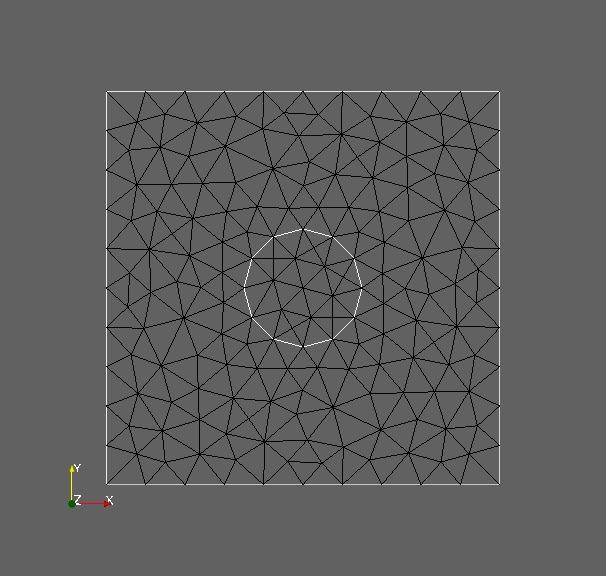
\includegraphics[scale=0.25]{pic_smallcircle.jpg}
	\caption{}	
	\end{subfigure}
	\begin{subfigure}{0.5\textwidth}
	\centering
	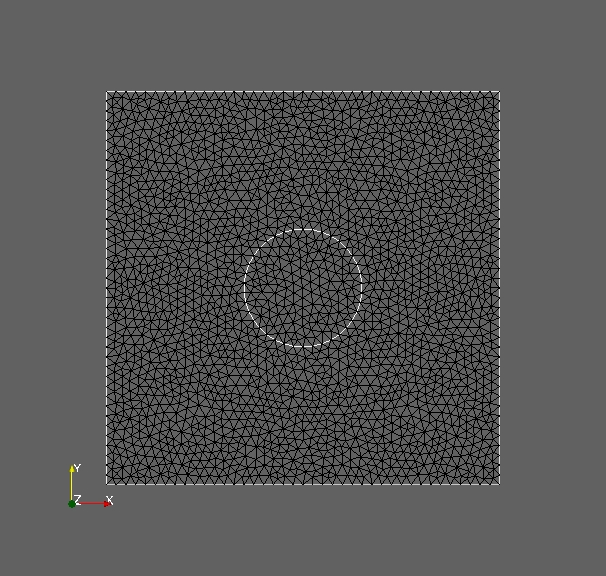
\includegraphics[scale=0.25]{pic_smallcircle_fine.jpg}
	\caption{}	
	\end{subfigure}
	\begin{subfigure}{0.5\textwidth}
	\centering
	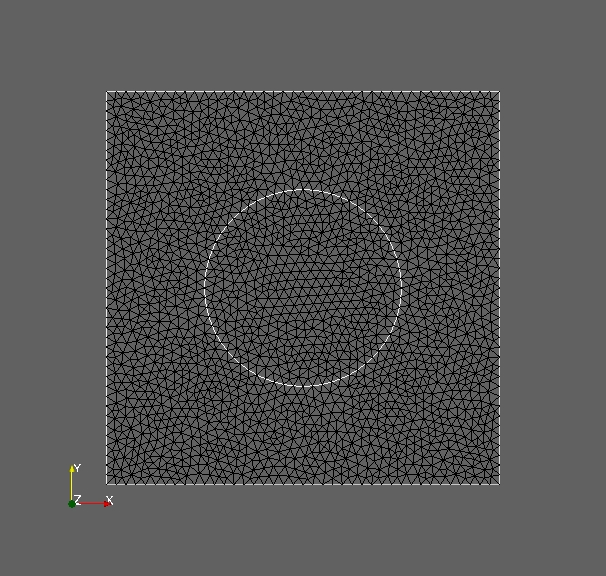
\includegraphics[scale=0.25]{pic_bigcircle_fine.jpg}
	\caption{}	
	\end{subfigure}
	\begin{subfigure}{0.5\textwidth}
	\centering
	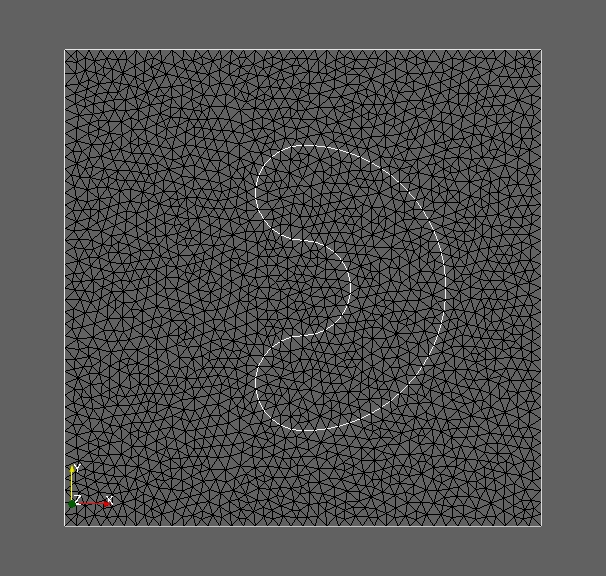
\includegraphics[scale=0.25]{pic_brokendonut_fine.jpg}
	\caption{}	
	\end{subfigure}
\caption{(a) Ausgangsform kleiner Kreis auf grobem Gitter (b) Ausgangsform kleiner Kreis auf feinem Gitter (c) Zielform großer Kreis auf feinem Gitter (d) Zielform broken Donut auf feinem Gitter}
\label{Meshes}
\end{figure}

Wir werden sowohl das L-BFGS-Verfahren, als auch das Gradientenverfahren vergleichen. Außerdem wird jeweils die Linesearch an- und ausgeschaltet, sowie alle oben aufgeführten Parameter, bis auf die Funktionswerte die Zustandsgleichung im Zielgitter, den Verbesserungsfaktor \textsf{c}, und den Skalierungsfaktor \textsf{shrinkage} der Backtracking-Linesearch, variiert. Die Verwendung der Memory-Length von 60 bewirkt, dass es sich in allen folgenden Fällen der Verwendung des L-BFGS-Verfahrens eigentlich um ein BFGS-Verfahren handelt, da die gesamte Historie zur Berechnung der Hesseapproximation benutzt wird. 

\subsection{Problem: kleiner zu großem Kreis}\label{subsect_circle}

Für das Problem der Deformation zum großen Kreis betrachten wir vor dem BFGS-Verfahren zunächst das Gradientenverfahren. Alle Zeiten und Anzahlen der benötigten Schritte der Verfahren finden sind in Tabelle \ref{Tabelle}. Wir erhalten bei dem groben Gitter 
bei Verwendung des Gradientenverfahrens ohne Linesearch Konvergenz nach fast 800 Schritten. Schaltet man das Backtracking ein, so erhält man ebenfalls Konvergenz, jedoch bei gut halber Anzahl der Schritte. Dies legt nahe, das die Schrittweite durch das anfangliche Hochskalieren der Deformation optimaler wird, der Gradient also der Norm nach relativ klein war. Bei Verfeinerung des Gitters um das 4-fache erhalten wir ebenfalls ohne Verwendung der Linesearch beim Gradientenverfahren Konvergenz nach ca. 650 Schritten, wobei wieder durch Verwendung des Backtracking eine Beschleunigung zur Konvergenz stattfindet. Die Konvergenzplots finden sich in Abbildung \ref{Konvplots_circle}. Erhöht man das anfängliche Hochskalieren vom Faktor 5 auf 20, so erhält man im feinen Gitter Konvergenz schon nach 120 Schritten. Die Geschwindigkeit zur Konvergenz hat sich also im Vergleich zum Gradientenverfahren ohne Backtracking also um das 5-fache gesteigert, wobei sich die erzeugten Gitter bei Ausstieg des Verfahrens mit oder ohne Linesearch und Veränderung des Hochskalierungsfaktors so gut wie nicht unterscheiden. 

\begin{table}[h]
\label{Tabelle}
\centering
\begin{tabular}{c rrrr}
\hline\\[-2.5ex]
 & \hspace{1cm} Zeit & & \hspace{1cm} Schritte \\
Problem &Gradientenv. &BFGS-Verf. &Gradientenv. &BFGS-Verf.  \\[0.2ex]

\hline \hline 
großer Kreis (grob) & 13,7s      & 4,8s       & 33      & 6 \\
großer Kreis (fein) & 1min 31,3s & 17,2s      & 52      & 7 \\
broken Donut (grob) & 43,3s$^*$  & 6,6s       & 109$^*$ & 9 \\
broken Donut (fein) & 27min 4,6s & 1min 25,4s & 910     & 27 \\
\hline
\end{tabular} 

\vspace{0.2cm}$^*$ \textit{Gradientenverfahren steigt bei Genauigkeit 0.0033 aus, weil \newline \hspace{-3.2cm}Linesearch keine Abstiegsrichtung findet}
 
 \caption{Rechendauern und Schritte der Verfahren (mit Backtracking-Linesearch)}

\end{table}


Findet das BFGS-Verfahren ohne Linesearch Anwendung, so erhält man auf dem groben Gitter keine Konvergenz. Das Verfahren updatet die BFGS-Memory nach mehreren Verletzungen der Curvature Condition nicht, und deformiert das Gebiet schließlich bei Schritt 26 bis zur Unbrauchbarkeit, was in Abbildung \ref{Destroyedbfgs_grob} zu sehen ist. Man beachte die starke Entartung der kaum sichtbaren Zellen kurz vor der Zerstörung des Gitters, welche man im Zoom gut erkennt.


\begin{figure}
	\begin{subfigure}{0.5\textwidth}
	\centering
	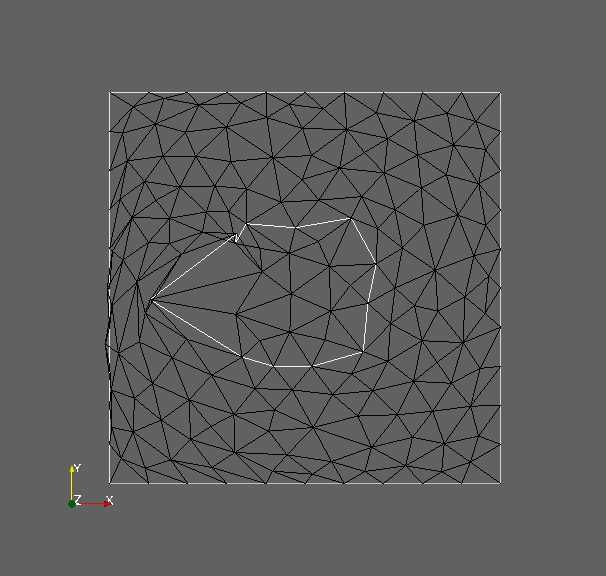
\includegraphics[scale=0.25]{pic_smallcircle_destroyed1.jpg}
	\caption{}	
	\end{subfigure}
	\begin{subfigure}{0.5\textwidth}
	\centering
	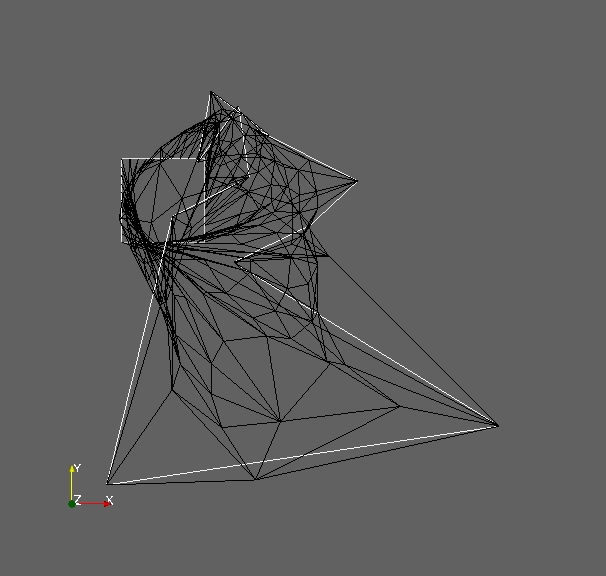
\includegraphics[scale=0.25]{pic_smallcircle_destroyed2.jpg}
	\caption{}	
	\end{subfigure}
\caption{(a) Gitter nach mehrmaligen Schritten unter Verletzung der Curvature Condition und Non-update Schritten (b) der darauf folgende Schritt, Zerstörung des Gitters}
\label{Destroyedbfgs_grob}
\end{figure}

Auch bei Verfeinerung des Gitters um das 4-fache erhält man keine Konvergenz des BFGS-Verfahrens, sondern erreicht die Zerstörung des Gitters nach Verletzung der Curvature Condition schon im zweiten Schritt, bei der die Form das Einheitsquadrat verlässt, siehe Abbildung \ref{Destroyedbfgs}. Man beachte, das dieses mal die Richtung des Schrittes in Richtung Optimum geht, jedoch viel zu lang ist, anders als in Abbildung \ref{Destroyedbfgs_grob}, wo zuvor mehrmalige falsche Schritte bei Verletzung der Curvature Condition das grobe Gitter zerstören. Diese Beobachtung macht erneut deutlich, wie wichtig eine effektive Schrittweitensteuerung bei der Implementierung der Verfahren ist.

\begin{figure}
	\begin{subfigure}{0.5\textwidth}
	\centering
	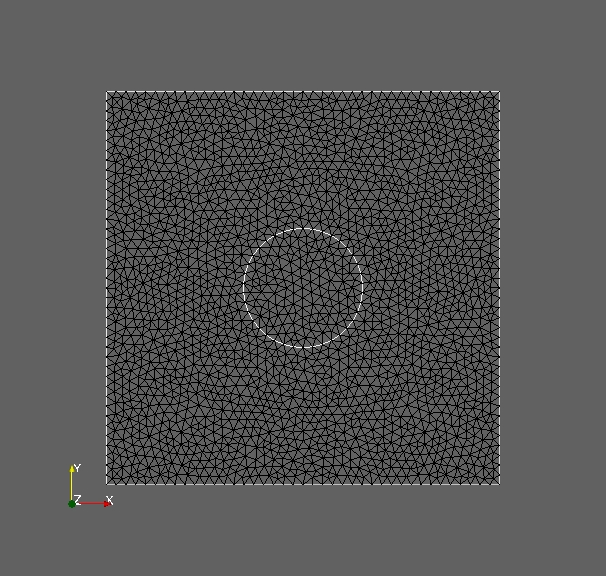
\includegraphics[scale=0.25]{pic_smallcircle_bfgsdestroyed1.jpg}
	\caption{}	
	\end{subfigure}
	\begin{subfigure}{0.5\textwidth}
	\centering
	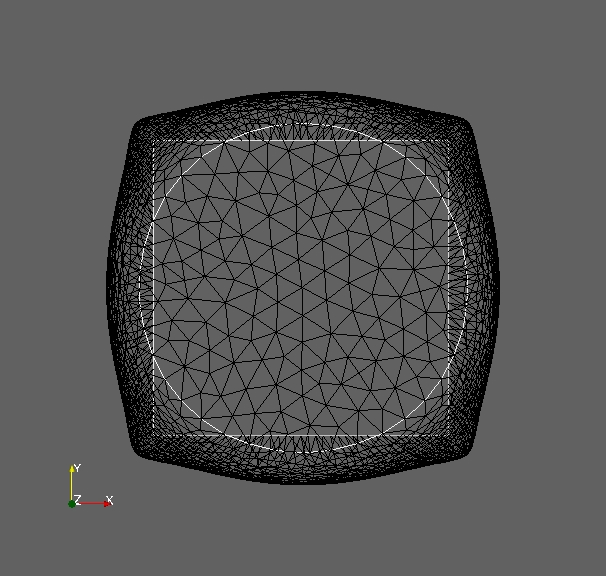
\includegraphics[scale=0.25]{pic_smallcircle_bfgsdestroyed2.jpg}
	\caption{}	
	\end{subfigure}
\caption{(a) 1. Schritt des BFGS-Verfahrens: Gradientenschritt bei feinem Gitter (b) 2. Schritt: BFGS-Schritt mit Entartung des feinen Gitters}
\label{Destroyedbfgs}
\end{figure}

Wir haben auch versucht, die Gitterzerstörung beim BFGS-Verfahren durch Modifikation der lokal variierenden Lamé-Parameter zu begegnen. Alle bisher gezeigten Gitter hatten die Wahl des minimalen Lamé-Parameters von 0. Um zu beobachten, ob die Verfahren instabiler werden, wenn man konstante Lamé-Parameter wählt, haben wir diese konstant auf 30 gesetzt. Man erhält den Output \ref{Destroyedkonstlame}, wobei bei Schritt 5 und 6 die Curvature Condition verletzt sind, und keine Linesearch verwendet wurde.

\begin{figure}
	\begin{subfigure}{0.3\textwidth}
	\centering
	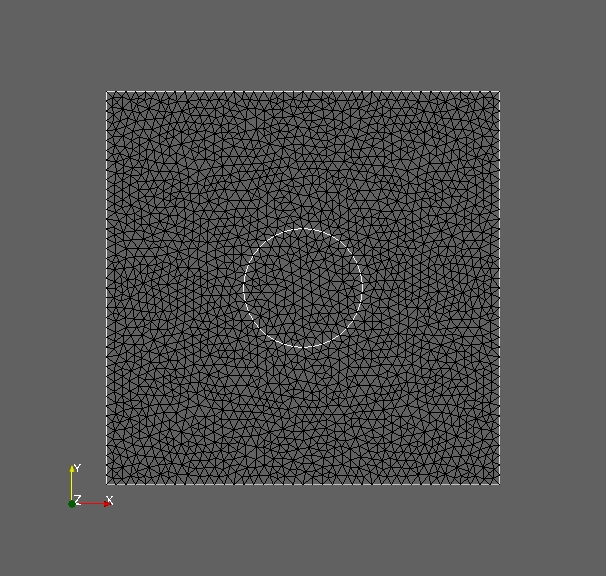
\includegraphics[scale=0.2]{pic_bigcircle_constlame1.jpg}
	\caption{}	
	\centering
	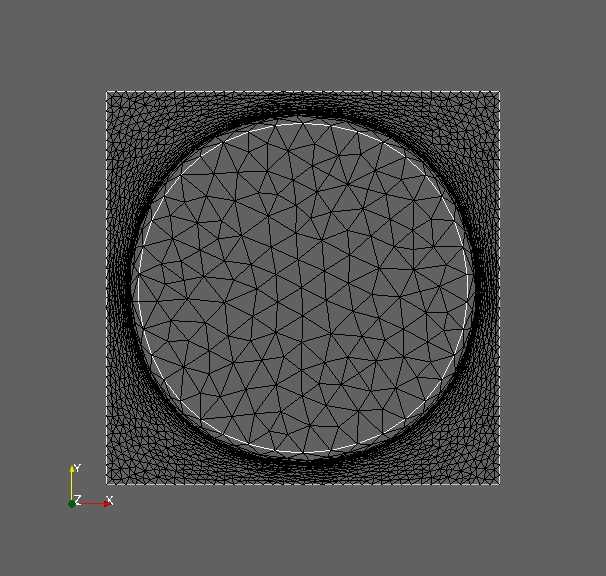
\includegraphics[scale=0.2]{pic_bigcircle_constlame2.jpg}
	\caption{}	
	\end{subfigure}
	\begin{subfigure}{0.3\textwidth}
	\centering
	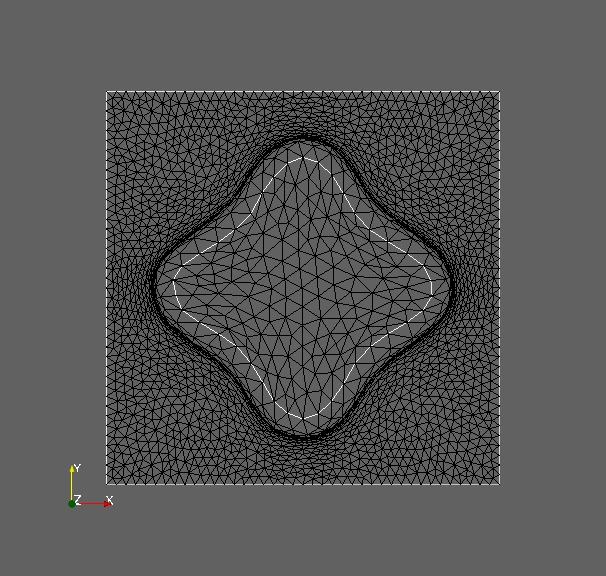
\includegraphics[scale=0.2]{pic_bigcircle_constlame3.jpg}
	\caption{}	
	\centering
	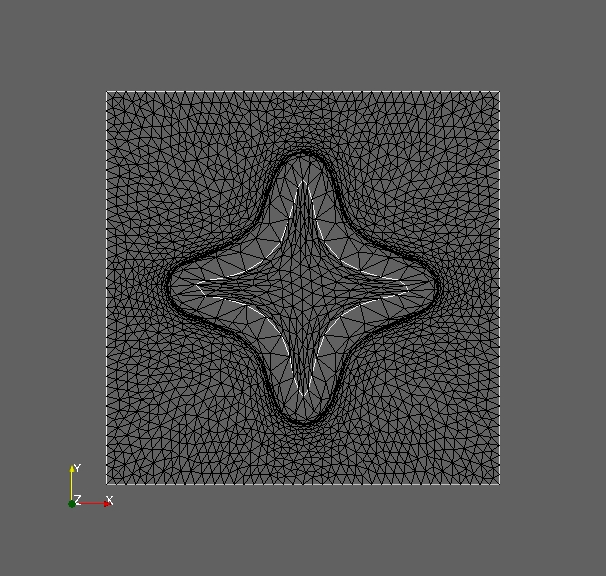
\includegraphics[scale=0.2]{pic_bigcircle_constlame4.jpg}
	\caption{}	
	\end{subfigure}
	\begin{subfigure}{0.3\textwidth}
	\centering
	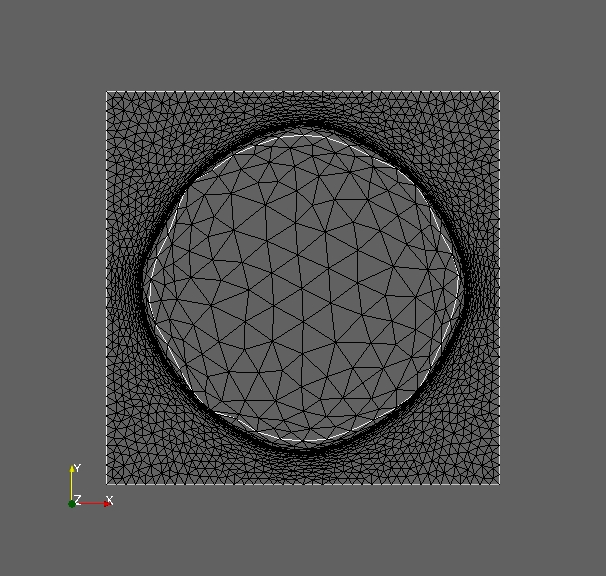
\includegraphics[scale=0.2]{pic_bigcircle_constlame5.jpg}
	\caption{}	
	\centering
	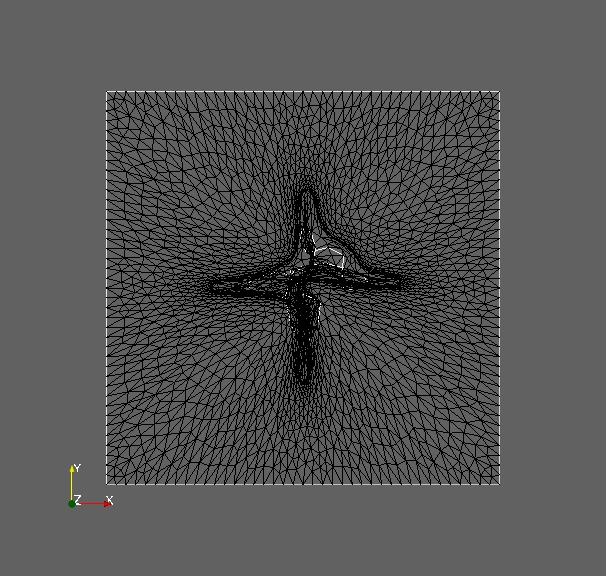
\includegraphics[scale=0.2]{pic_bigcircle_constlame6.jpg}
	\caption{}	
	\end{subfigure}
\caption{BFGS-Verfahren ohne Schrittweitensteuerung bei konstanten Lamé-Parametern mit Wert 30; die ersten 6 Schritte}
\label{Destroyedkonstlame}
\end{figure}

Ein komplett anderes Verhalten stellt sich bei Verwendung der Backtracking-Linesearch ein; in diesem Fall konvergiert das L-BFGS-Verfahren für beide Gitterfeinheiten.
Zudem fällt eine erhebliche Steigerung der Konvergenzgeschwindigkeit im Vergleich zum Gradientenverfahren auf; schon nach 5 Schritten auf dem groben, und nach 6 auf dem feinen Gitter. Die entsprechenden Konvergenzplots für die Verfahren mit Linesearch auf grobem und feinem Gitter sind zu sehen in \ref{Konvplots_circle}.

\begin{figure}
	\begin{subfigure}{0.5\textwidth}
	\centering
	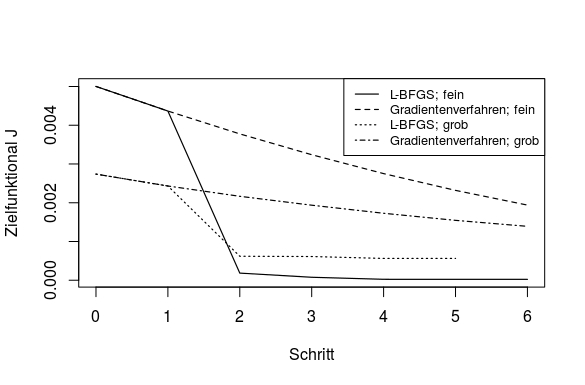
\includegraphics[scale=0.48]{plot_circle_target.jpeg}
	\caption{}	
	\end{subfigure}
	\begin{subfigure}{0.5\textwidth}
	\centering
	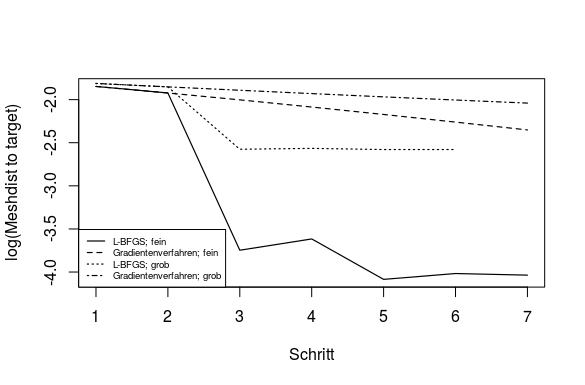
\includegraphics[scale=0.48]{plot_circle_meshdist.jpeg}
	\caption{}	
	\end{subfigure}
\caption{kleiner Kreis auf großer Kreis (a) Werte des Zielfunktionals bei den Verfahren mit Linesearch; unterschiedliche Gitterfeinheiten (b) logarithmierte Meshdistanz bei Verfahren mit Linesearch; unterschiedliche Gitterfeinheiten}
\label{Konvplots_circle}
\end{figure}

Die bei dem groben Gitter erzeugte optimale Form besitzt noch einen mit bloßem Auge sichtbaren Abstand zur Zielform. In diesem Fall hat unser L-BFGS-Algorithmus bei dem Backtracking maximal herunterskaliert, d.h. keine Abstiegsrichtung gefunden und ist ausgestiegen. Damit scheint ein lokales Minimum erreicht, zu sehen in Abbildung  \ref{Konvergenzbfgscircle} (a). Diese Vermutung liegt nahe, da die zugehörigen Werte der Norm der Formableitung \textsf{nrm\_f\_elas} gegen Null streben, hierzu verweisen wir auf die mitgelieferten Daten. Bei Verwendung des feinen Gitters ist bei selbem Ausstiegskriterium kein Abstand zur Zielform sichtbar, was man in Abbildung \ref{Konvergenzbfgscircle} (b) sehen kann.

\begin{figure}
	\begin{subfigure}{0.5\textwidth}
	\centering
	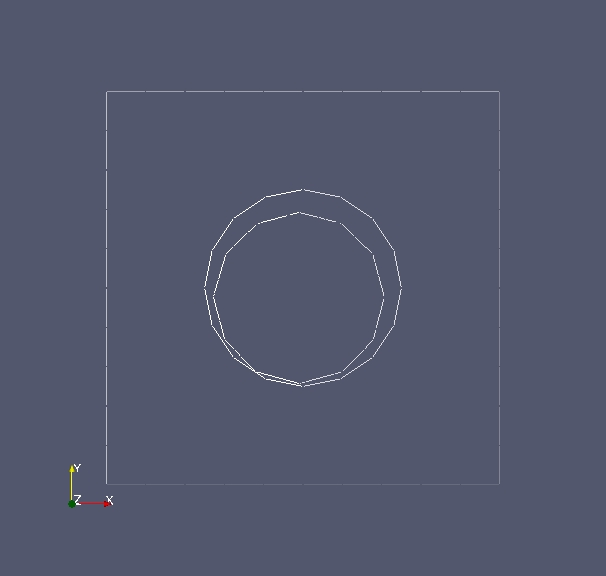
\includegraphics[scale=0.25]{pic_bigcircle_bfgs_linesearch.jpg}
	\caption{}	
	\end{subfigure}
	\begin{subfigure}{0.5\textwidth}
	\centering
	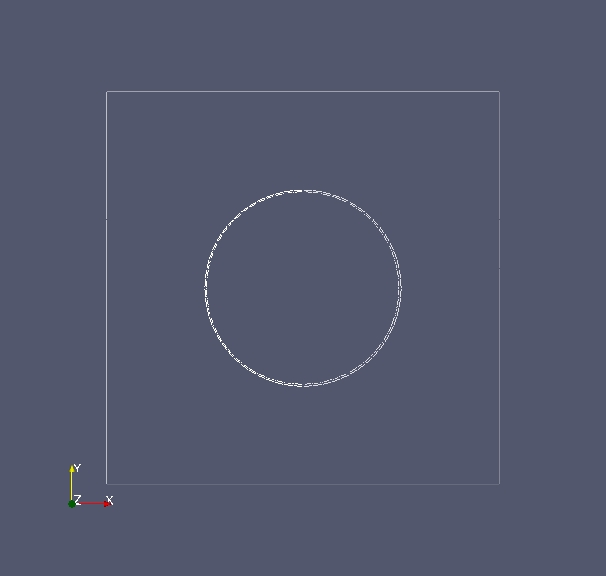
\includegraphics[scale=0.25]{pic_bigcircle_bfgs_linesearch_fine.jpg}
	\caption{}	
	\end{subfigure}
\caption{(a) L-BFGS mit Backtracking bei grobem Gitter. Abweichung bei Ausstieg sichtbar. (b) L-BFGS mit Backtracking bei feinem Gitter. Abweichung bei Ausstieg nicht erkennbar.}
\label{Konvergenzbfgscircle}
\end{figure}

Wir haben durch Veränderung der Perimeter-Regularisierung untersucht, ob sich durch diese der Abstand zur Zielform erklären lässt. Die Vermutung ist, dass die optimale Form etwas kleiner als die Zielform ist, da die Perimeter-Regularisierung kleinere Formen favorisiert. Die in diesem Fall entstehende optimale Lösung ist in diesem Fall symmetrisch mit gleichem Mittelpunkt wie die Zielform, jedoch besitzt sie fast den selben Abstand wie die optimale Form mit der Perimeterregularisierung aus Abbildung \ref{Konvergenzbfgscircle} (a). Für die exakten Bilder verweisen wir auf die mitgelieferten \textsf{.pvd}-Dateien auf der CD.

Kontrollieren wir im Falle des BFGS-Algorithmus auf Veränderung bei Erhöhung des Hochskalierungsfaktors \textsf{starscale} des Backtracking, so stellen wir fest, dass die ersten Schritte stärkere Verbesserungen bringen. Sobald sich jedoch eine gewisse Memorygröße, und damit eine Hesseapproximation, aufgebaut haben, verschwinden diese Effekte wieder, siehe Abbildung \ref{plot_startscales}. Dieses Verhalten sollte auftreten, da BFGS-Schritte mit aufgebauter Hesseapproximation skalierungsinvariant sind.

\begin{figure}
	\begin{subfigure}{0.5\textwidth}
	\centering
	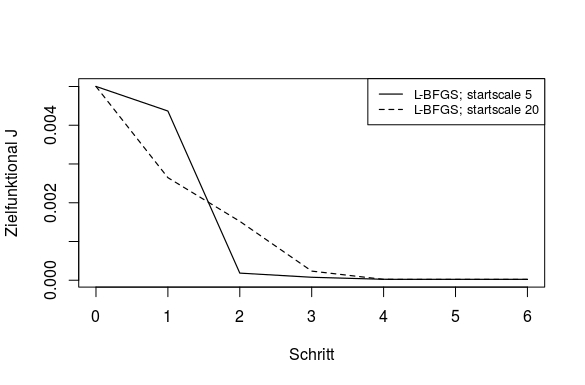
\includegraphics[scale=0.48]{plot_circle_bfgs_fine_startscale.jpeg}
	\caption{}	
	\end{subfigure}
	\begin{subfigure}{0.5\textwidth}
	\centering
	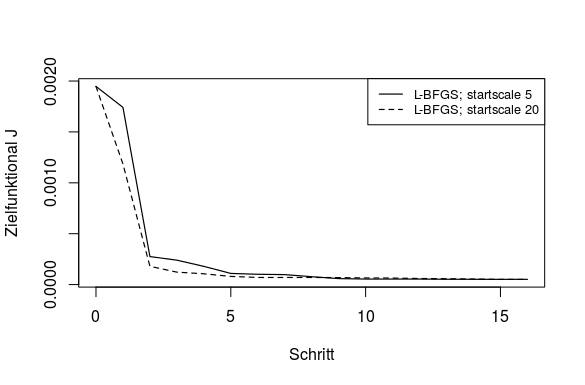
\includegraphics[scale=0.48]{plot_donut_bfgs_fine_startscale.jpeg}
	\caption{}	
	\end{subfigure}
\caption{Zielfunktional bei Variation des Skalierungsparameters \textsf{start\_scale} des Backtracking für das L-BFGS-Verfahren auf feinen Gittern der Probleme
 (a) kleiner Kreis auf großen Kreis (b) kleiner Kreis auf "broken  donut"}
\label{plot_startscales}
\end{figure}

Zudem haben wir einen Vergleich zwischen der vollen BFGS-Methode, welche wir durch die \textsf{memory\_length} von 60 erzeugen, und der echten Limited-Memory-BFGS-Methode, mit \textsf{memory\_length} von 2 und 3, im Falle des feinen Gitters gezogen. Interessanterweise stellt sich hier überhaupt kein Unterschied hinsichtlich Konvergenzgeschwindigkeit und erzeugte Werte im Zielfunktional ein, was man in Abbildung \ref{plot_memlen_lame} (a) erkennen kann. Ähnliche Beobachtungen machten die Autoren von \cite{diffusion} bei elliptischen und parabolischen Problemen, siehe das genannte Paper, Abschnitt 3. Dies lässt sich nach unserer Vermutung dadurch erklären, dass für einen korrekten BFGS-Schritt ein Term fehlt. Würde dieser ergänzt, so hoffen wir auf eine Verbesserung des Algorithmus bei höherer \textsf{memory\_length} auftreten sollte. Außerdem lässt sich in den Diagrammen keine asymptotische superlineare Konvergenz nachweisen, welche sich bei korrektem Update möglicherweise einstellt.

\begin{figure}
	\begin{subfigure}{0.5\textwidth}
	\centering
	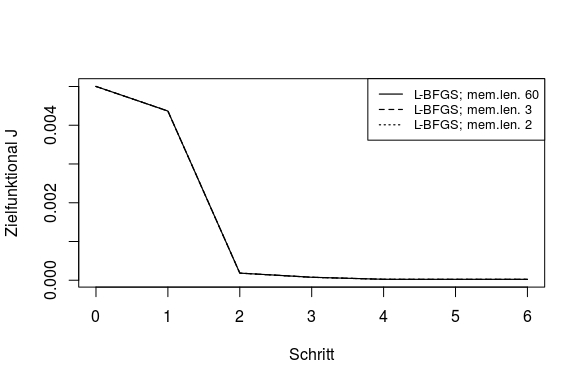
\includegraphics[scale=0.48]{plot_circle_bfgs_fine_memlen.jpeg}
	\caption{}	
	\end{subfigure}
	\begin{subfigure}{0.5\textwidth}
	\centering
	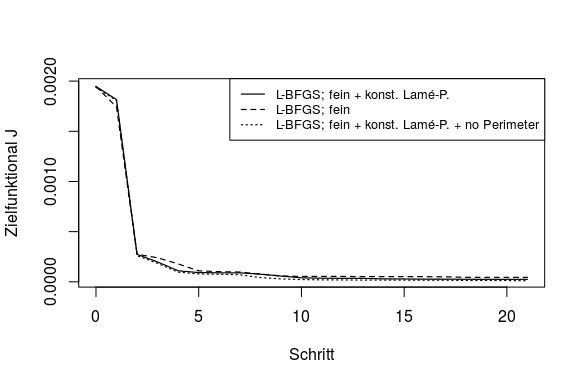
\includegraphics[scale=0.48]{plot_donut_bfgs_fine_lame.jpeg}
	\caption{}	
	\end{subfigure}
\caption{(a) Variation des L-BFGS-Parameters \textsf{memory\_length} bei feinem Gitter des Problems kleiner Kreis auf großer Kreis. Zu sehen sind 3 verschiedene Graphen, numerische Abweichungen treten erst ab Schritt 5 ab der 3 Nachkommastelle auf, weshalb diese fast gleich aussehen. \newline (b) Änderung der Lamé-Parameter und Entfernen der Perimeter-Regularisierung auf feinem Gitter des Problems kleiner Kreis auf "broken  donut".}
\label{plot_memlen_lame}
\end{figure}

Neben der bloßen Bedingung einer Verbesserung im Zielfunktional bei dem Backtracking besteht die Möglichkeit, die Armijo-Bedingung für die Linesearch zu verwenden. Diese haben wir nach \cite{Nocedal}, wie im Unterabschnitt  \ref{backtracking} gezeigt,  implementiert. Verwendet man diese, so konvergiert die L-BFGS-Method nicht mehr, in einigen Fällen konvergiert das Gradientenverfahren. Jedoch würde wir eher behaupten, dass dies \textit{trotz} der Armijo-Bedingung konvergiert. Da diese Bedingung die Verbesserung mit Hilfe eines linearen Modells in der aktuellen Form betrachtet, wäre ein aus der Formoptimierung legitimes anderes Modell vorstellbar, um verbesserte Bedingungen zur Linesearch zu erzeugen. Hierzu hat uns leider die Zeit gefehlt.

Bei der Berechnung des Formgradienten, wie im Unterabschnitt \ref{Berechnung_bib} erklärt, haben wir ein Verfahren verwendet, welches in der linearen Elastizitätsgleichung die Punkte, welche nicht Träger des inneren Randes sind, auf Null setzt. Schaltet man diese Nullsetzung aus, was durch die Wahl des Parameters \textsf{zeroed = False} möglich ist, so zerstört dies die Konvergenz des Verfahrens. Sowohl das L-BFGS, als auch das Gradientenverfahren divergieren in allen von uns getesteten Beispielen. Somit tritt der selbe Effekt wie in \cite{bfgs2}, welcher dort in Abschnitt 5, Fig. 2 zu sehen ist. Würde dieser Effekt durch ein Rundungsrauschen hervorgerufen sein, so vermuten wir, dass dieses weniger drastisch sichtbar würde. Bei uns ist schon nach den ersten Schritten das Gitter bis zur Unbrauchbarkeit entartet. Eine befriedigende Erklärung hierfür haben wir leider nicht.

\subsection{Problem: kleiner Kreis zu 'broken Donut'}\label{subsect_donut}

Wir haben die oben genannten Beobachtungen auch für das schwierigere Problem der nierenförmigen, nicht konvexen Form gesammelt. Die Ausgangsform, welcher den kleinen Kreis in Abbildung \ref{Meshes} (a) und (b) darstellt, bleibt gleich, wir wechseln also nur die Zielform, die auch in Abbildung \ref{Meshes} (d) zu sehen ist. 

Anders als bei dem einfacheren ersten Problem, erhalten wir für ein Gradientenverfahren ohne Backtracking-Linesearch, in den Fällen sowohl des groben, als auch des feinen Gitters, nach ca. 1200, respektive ca. 600 Schritten zwar Konvergenz, jedoch nicht zum globalen Optimum des Zielgitters. Wir vermuten, dass es sich hierbei um lokale Minima handelt, weil die Norm der Formableitung \textsf{nrm\_f\_elas} gegen $0$ geht, wobei wir auf die Daten verweisen. Die resultierende optimale Form bleibt konvex, trotz des nicht konvexen Zielgitters, siehe Abbildung
\ref{brokendonutgradient}. 

\begin{figure}
	\begin{subfigure}{0.5\textwidth}
	\centering
	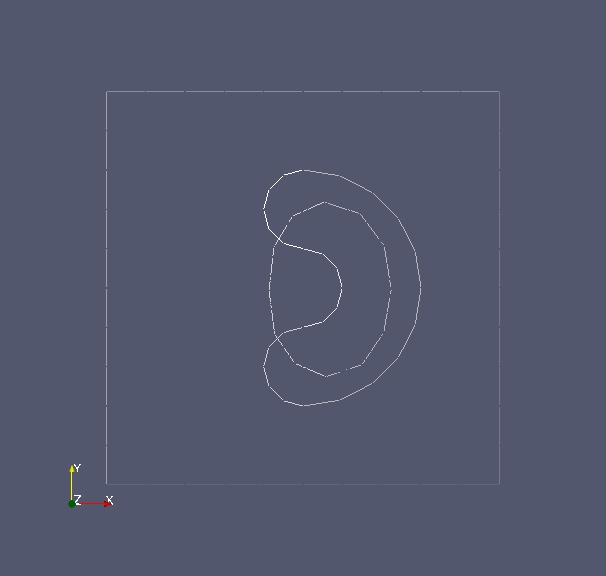
\includegraphics[scale=0.25]{pic_brokendonut_gradient.jpg}
	\caption{}	
	\end{subfigure}
	\begin{subfigure}{0.5\textwidth}
	\centering
	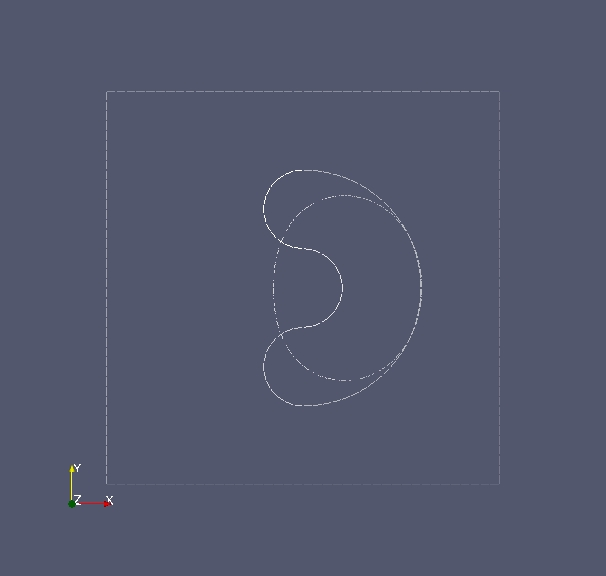
\includegraphics[scale=0.25]{pic_brokendonut_gradient_fine.jpg}
	\caption{}	
	\end{subfigure}
\caption{(a) Optimale Form und Zielform bei Gradientenverfahren auf grobem Gitter (b) Selbiges auf feinem Gitter}
\label{brokendonutgradient}
\end{figure}

Durch das Verwenden der Backtracking-Linesearch schafft es der Algorithmus näher an das globale Optimum zu gelangen. Dies gelingt jedoch ausschließlich bei dem feinen Gitter. Im Falle des groben Gitters erreichen wir auch mit Linesearch die selbe nicht konvexe Form, siehe Abbildung \ref{brokendonutgradient_linesearch}, wobei eine leichte Verbesserung zu sehen ist. Dies zeigt, dass das Verfahren abhängig von der Gitterfeinheit ist, wobei Verfeinerungen Verbesserungen liefern. Für die Zeiten und Schritte verweisen wir auf Tabelle \ref{Tabelle}.

Außerdem beobachten wir für das Gradientenverfahren, wie im ersten Problem, ein Skalieren der Konvergenzgeschwindigkeit durch das Hochskalieren der Suchrichtung bei der Backtracking-Linesearch. Wir sparen uns an dieser Stelle die Angabe eines Plots, da dieses Phänomen bekannt ist.
Zudem haben wir in diesem Problem die gleichen Feststellungen bei Verwendung der Armijo-Bedingung bei der Linesearch gemacht, wie bei dem ersten Problem zuvor.

\begin{figure}
	\begin{subfigure}{0.5\textwidth}
	\centering
	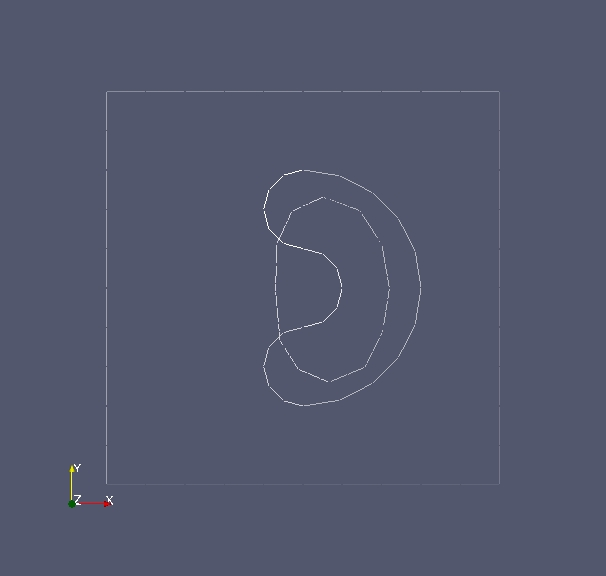
\includegraphics[scale=0.25]{pic_brokendonut_gradient_linesearch.jpg}
	\caption{}	
	\end{subfigure}
	\begin{subfigure}{0.5\textwidth}
	\centering
	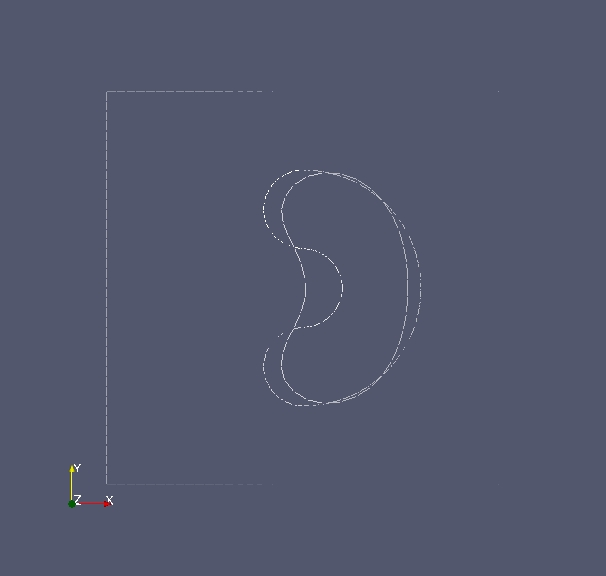
\includegraphics[scale=0.25]{pic_brokendonut_gradient_linesearch_fine.jpg}
	\caption{}	
	\end{subfigure}
\caption{(a) Optimale Form und Zielform bei Gradientenverfahren mit Linesearch auf grobem Gitter (b) Selbiges auf feinem Gitter}
\label{brokendonutgradient_linesearch}
\end{figure}

Bei Verwendung des L-BFGS-Verfahrens ohne Linesearch bemerken wir, ähnlich wie zu dem ersten Beispiel, dass sowohl beim groben, als auch beim feinen Gitter eine zu Abbildung \ref{Destroyedbfgs} ähnliche Divergenz stattfindet, weshalb wir uns Graphiken hierzu sparen. Das Gitter ist nach nur wenigen Schritten, nachdem die Curvature Condition verletzt wurde, bis zur Unkenntlichkeit verformt, wobei das Verfahren auch nicht die lokalen Minima \ref{brokendonutgradient_linesearch} oder \ref{brokendonutgradient} erreicht. 

\begin{figure}
	\begin{subfigure}{0.5\textwidth}
	\centering
	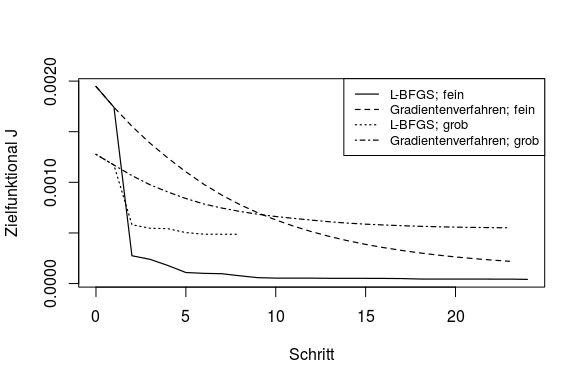
\includegraphics[scale=0.48]{plot_donut_target.jpeg}
	\caption{}	
	\end{subfigure}
	\begin{subfigure}{0.5\textwidth}
	\centering
	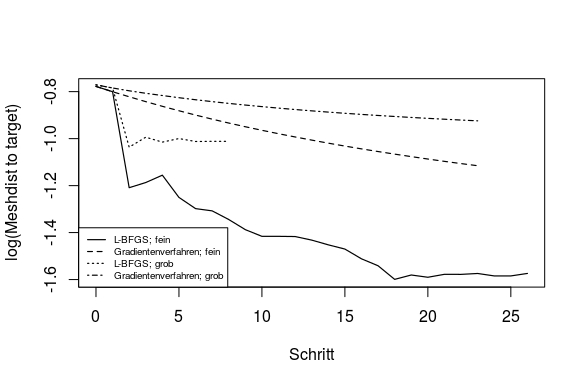
\includegraphics[scale=0.48]{plot_donut_meshdist.jpeg}
	\caption{}	
	\end{subfigure}
\caption{kleiner Kreis auf "broken donut" (a) Werte des Zielfunktionals bei den Verfahren mit Linesearch; unterschiedliche Gitterfeinheiten (b) logarithmierte Meshdistanz bei Verfahren mit Linesearch; unterschiedliche Gitterfeinheiten}
\label{plot_konvergenzdonut}
\end{figure}

Interessanterweise verbessert sich das Verhalten des L-BFGS-Verfahrens ohne Linesearch, wenn man statt lokal variierenden Lamé-Parametern konstante Lamé-Parameter mit Wert 30 wählt. Zuvor divergierte das Verfahren bei dem feinen Gitter nach nur 5 Schritten unter Verletzung der Curvature Condition der letzten 3 Schritte. Bei konstanten Lamé-Parametern findet zwar auch Divergenz statt, jedoch erst nach 14 Schritten, wobei zuvor sogar ein optimales Ergebniss, welches dem Gradientenverfahren mit Linesearch auf dem feinen Gitter nahe kommt, erreicht wird. Zu sehen sind ausgewählte Schritte in Abbildung \ref{brokendonut_bfgs_konstlame}. Man beachte jedoch den Vergleich zu dem Gitter, welches bei dem L-BFGS-Verfahren mit Linesearch und variierenden Lamé-Parametern erzeugt wird, bei dem geringere Entartung der Zellen des Gitters zu beobachten sind. Wir würden an dieser Stelle vorschlagen, ein Kriterium für die Entartung des Gitters, etwa dem Quotienten aus maximalem und minimalem Zellvolumen, zu verwenden, um bei Überschreitung eines festgelegten Entartungsgrades ein neues Gitter mit der aktuellen Form zu initialisieren. Dies ließe sich auch mit lokal variierenden Lamé-Parametern, sowie mit adaptiven Gittermethoden, kombinieren.

\begin{figure}
	\begin{subfigure}{0.315\textwidth}
	\centering
	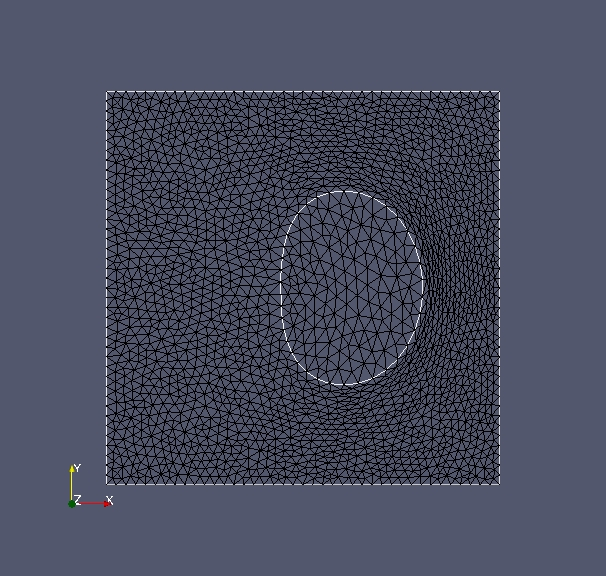
\includegraphics[scale=0.21]{pic_brokendonut_bfgs_konstlame_6.jpg}
	\caption{}	
	\end{subfigure}
	\begin{subfigure}{0.315\textwidth}
	\centering
	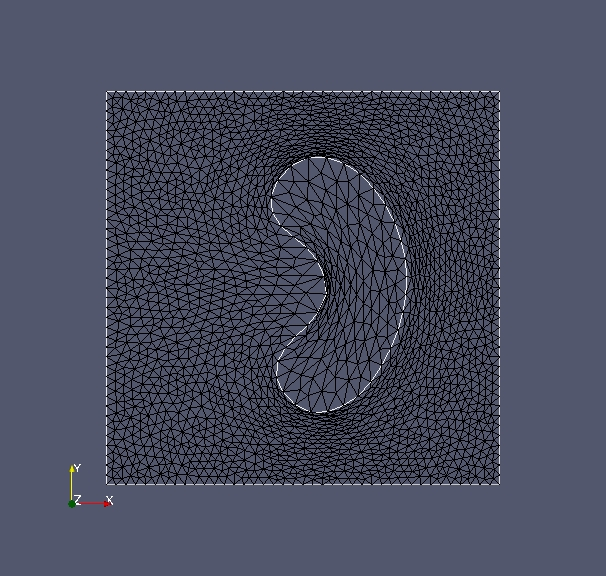
\includegraphics[scale=0.21]{pic_brokendonut_bfgs_konstlame_12.jpg}
	\caption{}	
	\end{subfigure}
	\begin{subfigure}{0.315\textwidth}
	\centering
	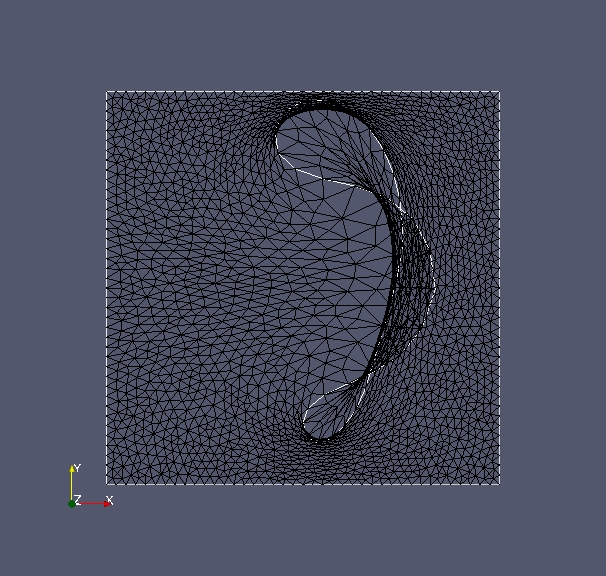
\includegraphics[scale=0.21]{pic_brokendonut_bfgs_konstlame_14.jpg}
	\caption{}	
	\end{subfigure}
\caption{BFGS-Verfahren bei konstanten Lamé-Parameter von 30 (a) Schritt 6 (b) gute Form bei Schritt 12; man beachte die starke Stauchung/ Streckung der Zellen (c) Zerstörung des Gitters bei Schritt 14}
\label{brokendonut_bfgs_konstlame}
\end{figure}

Verwendet man zusammen mit dem L-BFGS-Verfahren die Backtracking-Linesearch, so erhalten wir ähnliche Ergebnisse wie in dem ersten Problem, nähmlich eine deutliche Erhöhung der Konvergenzgeschwindigkeit im Vergleich zum Gradientenverfahren auf dem feinen Gitter. Auch auf dem groben Gitter ist eine erhebliche Erhöhung der Konvergenzgeschwindigkeit zu beobachten, wobei auch hier lediglich das lokale Minimum des Gradientenverfahrens erreicht wird. Auf dem feinen Gitter wird, ähnlich dem Gradientenverfahren mit Linesearch, eine sehr gute Lösung erreicht, nahe des globalen Optimums. Zu sehen sind die Ergebnisse des BFGS-Verfahrens mit Linesearch in Abbildung \ref{brokendonut_bfgs_linesearch}, für die Zeiten und Schritte verweisen wir erneut auf Tabelle \ref{Tabelle}. Bei dem Gradientenverfahren ist bei beiden untersuchten Problemen zu erkennen, dass eine deutliche Verfeinerung des Gitters keine Verlangsamung der Konvergenz mit sich bringt, was ein Indiz für gitterunabhängige Konvergenz ist, siehe Abbildung \ref{plot_konvergenzdonut} und \ref{Konvplots_circle}. Das BFGS-Verfahren weist zu schnelle Konvergenz auf, so dass wir hier keine Aussage über die gitterunabhängige Konvergenz machen können. 

Die Curvature Condition wird ab Schritt 17 verletzt, wobei schon in diesem Schritt eine fast vom Ergebniss kaum zu unterscheidbare Lösung erzeugt wird. Die Ausstiegsbedingung war somit lediglich zu stark gewählt, was man auch deutlich an dem Graphen aus Abbildung \ref{plot_konvergenzdonut} des feinen Gitters sehen kann. 

\begin{figure}
	\begin{subfigure}{0.5\textwidth}
	\centering
	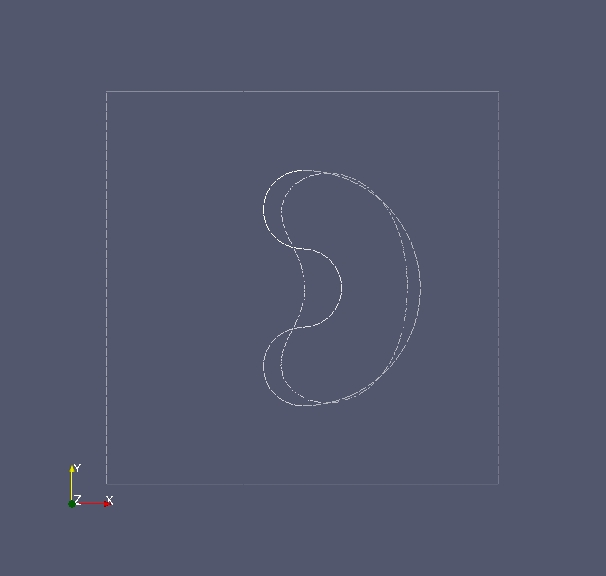
\includegraphics[scale=0.25]{pic_brokendonut_bfgs_linesearch.jpg}
	\caption{}	
	\end{subfigure}
	\begin{subfigure}{0.5\textwidth}
	\centering
	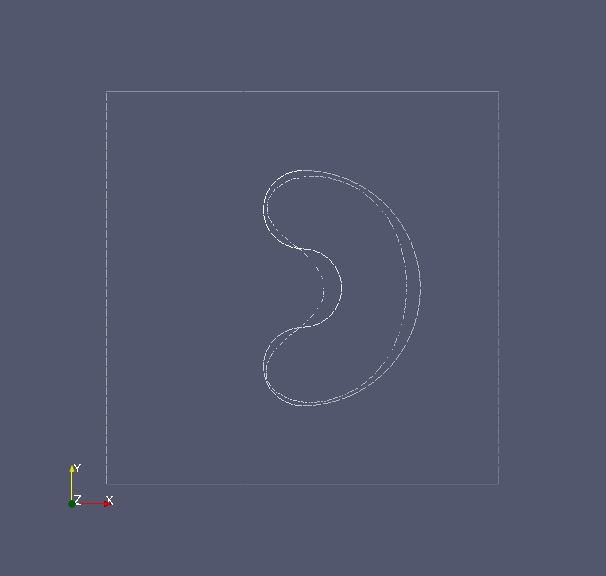
\includegraphics[scale=0.25]{pic_brokendonut_bfgs_linesearch_fine.jpg}
	\caption{}	
	\end{subfigure}
\caption{L-BFGS-Verfahren mit Linesearch (a) Form bei Ausstieg auf grobem Gitter (b) Form bei Ausstieg auf feinem Gitter}
\label{brokendonut_bfgs_linesearch}
\end{figure}


Weiterhin stellen wir fest, dass durch das Weglassen der Perimeter-Regularisierung die Konvergenz in diesem Problem erhalten bleibt, siehe den Graphen \ref{plot_memlen_lame} (b). Lässt man zusätzlich die Lamé-Paramter nicht lokal variieren, so bleibt auch hier die Konvergenz erhalten, das Verfahren benötigt jedoch etwas mehr als die doppelte Anzahl an Schritten bis die Toleranz an die Formableitung unterschritten wird. Betrachtet man die Konvergenzgraphen, fällt jedoch auf, dass dies an dem Ausstiegskriterium liegt, welches etwas zu stark gewählt ist. Somit funktioniert das Verfahren auch unter Anwendung konstanter Lamé-Parameter, sowie bei komplettem Weglassen der Perimeter-Regularisierung, erneut zu sehen in Abbildung \ref{plot_memlen_lame} (b). Allerdings liegt in allen Fällen ohne Linesearch Divergenz vor. Werden lediglich die Lamé-Parameter konstant gehalten, so tritt keine Änderung des Konvergenzverhaltens auf, was auch in Abbildung \ref{plot_memlen_lame} (b) zu sehen ist. Allerdings weisen die Zellen ohne lokal-variierende Lamé-Parameter einen höheren Entartungsgrad auf.

Außerdem beobachten wir, dass bei einer Memory-Length von 3, sprich bei einem echten Limited-Memory Ansatz, die Anzahl der benötigten Schritte zur Konvergenz von 26 auf 35 auf dem feinen Gitter steigt, jedoch bei dem groben Gitter gleich bei 8 Schritten bleibt. 

Zuletzt möchten wir anmerken, dass bei Betrachtung aller Konvergenzgraphen des BFGS-Verfahrens, sowohl des ersten Problems \ref{Konvplots_circle}, als auch des zweiten Problems \ref{plot_konvergenzdonut}, eine erhebliche, sprungartige Verbesserung im zweiten Schritt erfolgt. Wir vermuten, dass dies durch die Verwandtschaft des L-BFGS-Verfahrens mit dem CG-Verfahren erklärbar ist. Die Autoren von \cite{bfgsjumpconv} zeigen für die Minimierung quadratischer Zielfunktionen im $\mathbb{R}^n$ unter gewissen Bedingungen, dass alle Mitglieder der Broyden-Klasse, somit auch das BFGS-Verfahren, bei vollen Updates nach nur $n$ Schritten die Lösung erreichen. Verwenden die Autoren die Limited-Memory-Varianten, so verlieren alle Mitglieder der Broyden-Klasse diese Eigenschaft, mit einziger Ausnahme des L-BFGS-Verfahrens. Weiterhin zeigen die Autoren, dass bei der auch von uns angewandten Skipping-Strategie, dem Aussetzen von Updates bei Verletzung der Curvature-Condition, bei $q$-maligem Aussetzen immernoch ein Erreichen der Lösung nach nur $n+q$ Schritten vorliegt. Zwar haben die Autoren dies wie erwähnt für quadratische Funktionen im $\mathbb{R}^n$ gezeigt, unsere Beobachtungen bei den genannten Konvergenzgraphen legen jedoch ein ähnliches Verhalten in Kontext der Formoptimierung nahe. 

Wir beenden nun die Analyse der von uns erzeugten Daten, und laden die Leser dieser Arbeit gerne dazu ein, dass beiliegende Programm bei Interesse selber einigen Tests zu unterziehen. Abschließend möchten wir einen kleinen Ausblick auf mögliche weiterführende Themen und einige Probleme geben.

\subsection{Ausblick und Schlussbetrachtung}
Wir haben mit der in Kapitel \ref{Chapter_implementation} vorgestellten Implementierung, und den Ergebnissen aus den Abschnitten \ref{subsect_circle} und \ref{subsect_donut}, ein durchaus effektives Quasi-Newton-Verfahren in der Formoptimierung demonstriert. 
Die Konvergenzgeschwindigkeit im Vergleich zum Gradientenverfahren ist deutlich erhöht. Wir haben gesehen, dass eine Art der Schrittweitensteuerung, etwa dem bei uns implementierten Backtracking-Linesearch, für die Konvergenz des L-BFGS-Verfahrens nötig ist. An dieser Stelle gibt es Bedarf für weitere Entwicklungen; so wäre entweder eine im vorigen Kapitel angesprochene Verbesserung des Kriteriums für hinreichend gute Abstiege, die ein aus dem Formkalkül legitimes Modell für das Zielfunktional verwenden, denkbar. Diese könnte im Falle eines linearen Modells das Armijo-Kriterium auf Formräume verallgemeinern. Eine andere Variante wäre die Verwendung einer Art Trust-Region-Methode, mit dessen Hilfe auch eine globale Konvergenz erreicht werden könnte. Zudem kann sich mit diesem Ansatz die Möglichkeit bieten, durch das Vermeiden der Indefinitheit der Quasi-Newton-Approximation andere Verfahren, etwa den Broyden-SR1-Update, anwenden zu können. In den Konvergenzgraphen sind außerdem deutliche Verbesserungen nach nur wenigen Schritten zu erkennen, welche zuvor versucht haben zu erklären, und eine Ähnlichkeit zum CG-Verfahren ausweisen. Eine Limited-Memory-Variante des CG-Verfahrens für die Formoptimierung wäre eine weitere Möglichkeit dem zuvor genannten Problemen zu begegnen. Außerdem haben wir keine asymptotisch superlineare Konvergenz beobachten oder zuverlässig widerlegen können. Um dies anzugehen, wäre eine Anpassung der BFGS-Updates wichtig. Wie sich diese konkret im Formraum realisieren lassen, ist jedoch bis dato unklar. Wir haben weiterhin Indizien für gitterunabhängige Konvergenz bei Untersuchung des Gradientenverfahrens bemerkt, so dass es sich lohnenswert erscheint, das Verhalten der Verfahren bei anderen Problemen und anderer Wahl der Bilinearform $a$ und der damit erhaltenen Metrik $g^S$ zu analysieren. Eine Möglichkeit hierfür würde die biharmonische Gleichung bieten. Abschließend bleibt noch das etwas ominöse Problem bei Erzeugung der Formgradienten, bei dem ohne Nullsetzen der Punkte ohne Träger am inneren Rand zur Lösung der linearen Elastizitätsgleichung die verheerenden Effekte auftreten, welche das Gitter zerstören und wir nicht befriedigend erklären können. Dies sind viele mögliche Ansätze für kommende  Fortschritte im Bereich der Formoptimierung. Wir hoffen, mit dieser Arbeit einen kleinen Beitrag in die richtige Richtung geben zu haben, und bedanken uns bei Prof. Volker Schulz für die Möglichkeit diese Masterarbeit anzufertigen.
\newpage
\nocite{*}
\bibliographystyle{plain}
\bibliography{papers}

\end{document}


\newpage
\appendix
\section{Eidesstattliche Erklärung}
Hiermit erkläre ich, dass ich die Masterarbeit selbständig verfasst und keine anderen als die angegebenen Quellen und Hilfsmittel benutzt und die aus fremden Quellen direkt oder indirekt übernommenen
Gedanken als solche kenntlich gemacht habe. Die Masterarbeit habe ich bisher keinem anderen Prüfungsamt in gleicher oder vergleichbarer Form vorgelegt. Sie wurde bisher auch nicht veröffentlicht.
\vspace{1.5cm}
\today \newline
(Datum) \hspace{9cm} (Daniel Luft)


\newpage
\nocite{*}
\bibliographystyle{plain}
\bibliography{papers}

\end{document}